%% paper04 --- standalone short paper (English)
%% Template: ACM acmart, manuscript.  The body is decoupled from the earlier
%% NOSR/HMACSP narrative; only the layout skeleton is retained.
%% Compile: pdfLaTeX or XeLaTeX.  This version carries no CJK text, so the
%% ctex package of the Chinese manuscript is not loaded.
%%
\documentclass[manuscript,screen,review]{acmart}

\usepackage{algorithm}
\usepackage{algorithmicx}
\usepackage{algpseudocode}
\usepackage{pifont}
\usepackage{makecell}
\providecommand{\checkmark}{\ding{51}}
%% B13 dropped \cmark/\xmark/\omark: once defined they were never used in the
%% manuscript (the tables do not use a tick/cross convention).  Old values: git.
\usepackage{threeparttable}
\usepackage{tikz}
\usetikzlibrary{positioning,arrows.meta,calc,shapes,shadows}
\usepackage{xcolor}
\usepackage{amsmath}
\usepackage{bm}
\DeclareMathOperator*{\argmin}{arg\,min}
\DeclareMathOperator*{\argmax}{arg\,max}
\usepackage{multirow}
\usepackage{enumitem}
\usepackage{booktabs}
\usepackage{graphicx}
\setlength{\headheight}{20.48303pt}

%% Printed names of the floats and theorem-like environments.
\renewcommand{\figurename}{Figure}
\renewcommand{\tablename}{Table}
\floatname{algorithm}{Algorithm}
\renewcommand{\proofname}{Proof}

%% Abbreviation of the mechanism: the subject is a closure, not a "repair
%% framework".
\providecommand{\STRC}{\textsc{STRC}}
%% B13 dropped \TBD: never used in the manuscript.  Items still to be supplied
%% are marked in plain text as <to be supplied: ...> so that a self-check can
%% grep for them.

%% =====================================================================
%% Single source for the headline numbers.
%%
%% All of them are printed by STRC/tools/paper_numbers.py from
%% STRC/experiments/expanded/*.csv, whose data are produced by
%% `py -m tools.expand_batch` (5 instances x 10 seeds by default).
%% The prose always cites a macro and never a literal; to change a number,
%% change it here only, then re-run the two commands above and check.
%%
%% !! 2026-08-16: the batch grew from 3x5=15 pairs to 5x10=50 pairs.  Every
%% !! /15 reading of the old manuscript is therefore void.
%%
%% !! 2026-08-16 (second pass): E2b went from 24/50 to 50/50.  This is not a
%% !! change of instances but the repair of a mismatch between implementation
%% !! and definition.  The release set is a set of *reservations*, whereas
%% !! replay_reroute used to decide rerouting per *operation* (if either leg
%% !! entered the closure, the whole transport was replanned).  So when only
%% !! the loaded leg entered the closure, the empty leg of the same operation
%% !! was rewritten as well, even though its task was not in the release set,
%% !! and this was recorded as drift outside the set.  The 84 drifting
%% !! reservations on the 26 failing cells were, without exception, empty legs
%% !! of this kind, and 71 of them (85%) had already finished before t_now ---
%% !! rewriting such a leg also violates Assumption A2.  Deciding per leg
%% !! instead drove the drift to zero.  Only then is premise (iii) of
%% !! prop:outside genuinely satisfied; the earlier 24/50 measured an
%% !! implementation defect, not the physical coverage of the edge set.
%% =====================================================================
\newcommand{\NInst}{5}
\newcommand{\NSeeds}{10}
\newcommand{\NPairs}{50}
%% E1/E3: both are full marks, written as \NPairs/\NPairs so that a hand-copied
%% number cannot go stale.
\newcommand{\PassMiss}{\NPairs/\NPairs}      % T_impact=0, seeds non-empty, original solution infeasible
\newcommand{\FeasRone}{0/\NPairs}            % cells on which R1 restores feasibility
\newcommand{\FeasRtwo}{\NPairs/\NPairs}      % cells on which R2 restores feasibility
\newcommand{\PassClosed}{\NPairs/\NPairs}    % E2a structural closedness (zero leakage)
\newcommand{\PassInvar}{\NPairs/\NPairs}     % E2b fields outside the set unchanged entry by entry
%% Per-instance extremes of Cl/|R| in the main E1 batch; source: the body of
%% tab:e1 (0.59/0.57/0.59/0.57/0.56).
%% This range used to be written with a different value at each of three places
%% in the prose (0.56--0.59 / 0.54--0.57 / 0.54--0.58), i.e. CONFLICT-3; it now
%% comes from these macros only.  Do **not** mix it with the following
%% numerically equal but differently sourced quantities:
%%   \ScaleCloHi(0.56) comes from the k=4 cell of the scale sweep tab:scale,
%%     which is a different batch;
%%   \PubEoneFracLo/Hi come from the external-layout batch, a separate ledger.
\newcommand{\EoneCloLo}{0.56}
\newcommand{\EoneCloHi}{0.59}
%% Runtime (E3 batch, level-1 rerouting, no scope escalation)
\newcommand{\MsRepairMed}{3.2}
\newcommand{\MsRepairMax}{12.8}
%% Stability: on E5, once Assumption A2 is enforced, the rewrite fractions of
%% the two arms fall in the same range; the headline contrast is now E7's
%% R2 vs RA.
\newcommand{\ResFracRtwo}{50\%--66\%}
%% E5 batch: R0+ now uses fixed-prefix decoding.  After a downgraded downstream
%% operation is made to continue on the same vehicle, all 18 budget points show
%% zero violations.
%% Source expanded/e5_cross_curve.csv, `py -m tools.expand_batch --only-e5`.
\newcommand{\RzeroPastLo}{0}
%% ---------------------------------------------------------------------
%% The two E5 batches are read together.  pub_batch imports _run_e5 from
%% expand_batch directly, and t_now_frac=0.35, budgets {0.2,1,2}s, pop=40 and
%% hot=True are identical item by item, so the two may be pooled; they differ
%% only in the provenance of the layouts (self-designed / externally
%% transcribed), which is exactly the point of pooling them.
%% Source expanded/e5_cross_curve.csv + pub_layouts/e5_cross_curve.csv,
%% recomputation script tools/_p17_e5_stats.py.
\newcommand{\EfiveInst}{4}          % congested_8x4x4, example_3x3x2, LyuL2_4m, LyuL6_8m
\newcommand{\EfiveCells}{12}        % instance--seed cells
\newcommand{\EfivePts}{36}          % budget points in total = 12 cells x 3 levels
\newcommand{\EfiveWLT}{35/1/0}      % R0+ win/tie/loss, budget point by budget point
\newcommand{\EfiveWinMin}{11}       % cells on which R0+ is strictly better at the smallest budget
\newcommand{\EfiveTieMin}{1}        % ditto, cells that tie (LyuL6_8m, seed 2024)
%% ---------------------------------------------------------------------
%% Dispersion convention (P17).  Every table or figure of means is accompanied
%% by an interquartile range, so that the reader does not see the mean alone.
%% Source: the script above; E1 from expanded/e1_miss.csv, 10 seeds per instance.
\newcommand{\EoneFracIqrLo}{0.024}  % smallest per-instance IQR of Cl/|R|
\newcommand{\EoneFracIqrHi}{0.049}  % ditto, largest
\newcommand{\EoneFracMed}{0.571}    % median over the 50 pooled pairs
%% The pooled IQR measures 0.0372, numerically equal to but \emph{sourced
%% differently from} the Hodges--Lehmann estimate 0.037 of Section 6.  To keep
%% two unrelated quantities from colliding into one reading in the prose, no
%% macro is defined here and the figure caption does not report it either;
%% reporting the per-instance IQR range and the pooled spread suffices.
\newcommand{\EoneFracMin}{0.500}    % lower end of the spread over the 50 pooled pairs
\newcommand{\EoneFracMax}{0.655}    % ditto, upper end
%% phi sweep (tab:scale / fig:scale): spread of the runtime and per-level IQR of Cmax
\newcommand{\ScaleMsMin}{2.2}       % lower end of strc_wall_ms over the whole sweep
\newcommand{\ScaleMsMax}{23.8}      % ditto, upper end
\newcommand{\ScaleCmaxIqrLo}{8}     % smallest per-level IQR of R0+ Cmax
\newcommand{\ScaleCmaxIqrHi}{76}    % ditto, largest
%% Runtime-ratio range of the scale sweep (per-cell extremes across two instances)
\newcommand{\SpeedLo}{87}
\newcommand{\SpeedHi}{3051}
%% E6: cells on which the closure is strictly larger than the release set
%% induced by the operation-precedence graph (on the remaining cells the two
%% are equal, which is not a containment failure)
\newcommand{\StrictlyLarger}{87/100}
%% E6: share of the closure in the occupancies still alive after t_now
%% (corridor blockage).  This number is large; it is the measured basis of the
%% remark that "no minimality is claimed", and must not be prettified.
\newcommand{\ClosureAliveFrac}{92\%}
%% =====================================================================
%% Externally sourced layout batch (STRC/experiments/pub_layouts/).  A
%% **separate ledger**: it is not merged into the \NPairs pairs above, since
%% mixing it into the main batch would change the convention behind every
%% /\NPairs reading.  The two batches are matched parameter for parameter and
%% differ only in the provenance of the layouts.  Source: py -m tools.pub_batch
%% followed by py -m tools.paper_numbers.
%% The edge weights are the uniform values supplied by this paper, so these
%% numbers **cannot** be compared with the reference values of Lyu or van Os.
%% =====================================================================
\newcommand{\NPubInst}{5}
\newcommand{\NPubPairs}{50}
\newcommand{\PubPassMiss}{\NPubPairs/\NPubPairs}
\newcommand{\PubFeasRone}{0/\NPubPairs}
\newcommand{\PubFeasRtwo}{\NPubPairs/\NPubPairs}
\newcommand{\PubPassClosed}{\NPubPairs/\NPubPairs}
\newcommand{\PubPassInvar}{\NPubPairs/\NPubPairs}
\newcommand{\PubEoneFracLo}{0.438}
\newcommand{\PubEoneFracHi}{0.547}
%% E4 like-for-like comparison.  **The convention here needs particular care;
%% it was once stated wrongly.**
%% The \NPubInst external instances live on only \NPubNets distinct road
%% networks (4x4 with one edge removed: LyuL2/L3; 5x5 with two edges removed:
%% LyuL4/L5/L6); they differ in the number of machines and in where the
%% machines sit.  Hence:
%%   the two endpoints of the spread \PubCloSpread (\PubCloHi = LyuL2 with 4
%%   machines, \PubCloLo = LyuL3 with 5 machines) **share one and the same
%%   network**, so the spread measures machine placement, **not** network
%%   geometry.
%%   Do not write this as "the closure share varies markedly with the layout"
%%   again --- the data do not support that sentence.
%% The correct use is: changing the placement on one and the same network
%% already yields \PubCloSpread, while the LU minimum cut and the funnel share
%% stay constant throughout (both networks put the load/unload station at a
%% grid corner, and under 4-adjacency a corner has exactly two outgoing
%% edges), so the static cut is cleanly refuted.
%% Careful not to phrase this as "public layouts always sit at a corner": the
%% Liu family shipped with the same toolset places it at the midpoint of a grid
%% edge (out-degree 3), and was left out only because it permits diagonal
%% moves.  The accurate statement is that this measure takes only a handful of
%% discrete values, all fixed by where the station is placed.
\newcommand{\NPubNets}{2}
\newcommand{\PubCloLo}{0.305}
\newcommand{\PubCloHi}{0.512}
\newcommand{\PubCloSpread}{0.207}
\newcommand{\PubCloSpreadBig}{0.075}
\newcommand{\SelfCloLo}{0.446}
\newcommand{\SelfCloHi}{0.497}
\newcommand{\SelfCloSpread}{0.051}
\newcommand{\PubEfiveNoCross}{17/18}
%% =====================================================================
%% Cheap comparison arms (E7) and instance-scale sweep (E8).  The two batches
%% share one set of arm definitions:
%%   RS  global right shift.  Paths, assignment and sequence are untouched;
%%       everything unfinished is pushed uniformly past the blockage window.
%%       The freezing criterion is the same as R2's (t_end <= t_now is
%%       immovable), so it is admissible under A2.
%%   RD  re-decoding of the original chromosome.  Machine assignment and sweep
%%       order are kept, and the same fixed-prefix decoding as R0+ is used.
%%       After a downgraded downstream operation is made to continue on the
%%       same vehicle, the A2 violations are \RedecodeBad.
%%   RA  no boundary at all: release every reservation after t_now, then run
%%       exactly the same rerouting replay as R2.  It shares the engine and
%%       the freezing criterion with R2, the only difference being that the
%%       release set is taken to be the trivial upper bound, so the whole of
%%       the R2--RA difference is attributable to the closure as an object.
%% Source: STRC/experiments/cheap_baselines.csv (py -m tools.cheap_baselines)
%%         STRC/experiments/scale_curve.csv     (py -m tools.scale_curve)
%% The protocol matches E1--E3 (single-window blockage on a busy corridor,
%% t_now=0.35 Cmax, no scope escalation for R2), so tab:cheap may be read
%% alongside tab:e3; it may **not** be read alongside tab:e5, which covers
%% two instances only.
%% =====================================================================
\newcommand{\MsShift}{1.42}          % median RS runtime/ms (\NPairs pairs)
\newcommand{\MsRedecode}{4.16}       % median RD runtime/ms (ditto)
\newcommand{\MsAllFuture}{2.76}      % median RA runtime/ms (ditto)
\newcommand{\MsCheapRtwo}{2.74}      % median R2 runtime in the same batch, for a like-for-like comparison of the four arms
\newcommand{\RedecodeRatio}{1.5}     % MsRedecode / MsCheapRtwo
\newcommand{\ShiftBad}{0/\NPairs}    % cells on which RS rewrites a finished reservation
\newcommand{\RedecodeBad}{0/\NPairs}
\newcommand{\WinVsShift}{27/16/7}    % R2 vs RS on Cmax, win/tie/loss
\newcommand{\WinVsRedecode}{14/14/22}
\newcommand{\WinVsAllFuture}{4/46/0}
\newcommand{\ResFracCheapRtwo}{0.540}
\newcommand{\ResFracShift}{0.627}
\newcommand{\ResFracRedecode}{0.618}
\newcommand{\ResFracAllFuture}{0.604}
%% Per-cell stability comparison of R2 against RA (rewrite fraction; all
%% \NPairs cells on which both arms are feasible are included).
\newcommand{\RAStabWTL}{31/18/1}     % R2 more stable/tie/less stable
\newcommand{\RAStabP}{8.8\times10^{-7}}  % Wilcoxon signed-rank, two-sided
\newcommand{\RAStabMean}{0.064}      % mean reduction in the rewrite fraction
%% The next two are the same readings after removing the 6 cells on which the
%% two methods coincide (R2's release set = all unfinished occupancies); they
%% are computed directly from cheap_baselines.csv by STRC/tools/audit_checks.py.
%% Removing those cells makes the reduction larger.
\newcommand{\RAStabWTLNet}{31/12/1} % R2 more stable/tie/less stable after removing the coincident cells (n=44)
\newcommand{\RAStabMeanNet}{0.073}  % ditto, mean reduction
\newcommand{\RAStabMed}{0.029}       % ditto, median reduction
\newcommand{\RACmaxRatio}{0.999}     % mean Cmax ratio R2/RA
\newcommand{\RACmaxLo}{0.970}        % ditto, minimum (the cell where R2 is most favoured)
\newcommand{\ClosureShareLo}{0.80}   % closure / all future reservations: minimum
\newcommand{\ClosureShareMean}{0.92} % ditto, mean (same source as \ClosureAliveFrac)
%% Instance-size ladder: 2k jobs, k machines, k vehicles, k=4..10; congestion
%% level, H, F, Tt/Tp and the two cut sets follow one and the same calibration,
%% and only the size varies (for the calibration of the generator
%% clbs/tools/gen_instances.py see its docstring).
\newcommand{\ScaleKs}{7}
\newcommand{\ScalePairs}{70}
\newcommand{\ScaleJobsHi}{20}
\newcommand{\ScaleMachHi}{10}
\newcommand{\ScaleCloLo}{0.48}       % closure as a share of the whole table: k=10
\newcommand{\ScaleCloHi}{0.56}       % ditto, k=4
%% The next three and the previous two are two denominators over the same data,
%% computed directly by tools/audit_checks.py from the n_res / n_live / closure
%% columns of scale_curve.csv (not back-derived).  The attainable upper bound of
%% Cl/|R| is |R^o|/|R|, so answering "can the share rise towards 1" requires
%% the Cl/|R^o| convention.
\newcommand{\ScaleAliveShare}{0.61}  % mean |R^o|/|R|, 0.611 averaged over the seven levels
\newcommand{\ScaleCloAliveLo}{0.78}  % closure as a share of the unfinished occupancies, lowest level mean: 0.782 at k=10
\newcommand{\ScaleCloAliveHi}{0.91}  % ditto, highest: 0.905 at k=4
\newcommand{\ScaleMsHi}{10.4}        % median R2 runtime: k=10
\newcommand{\ScaleRatioLo}{1.5}      % RD/R2 runtime ratio: k=4
\newcommand{\ScaleRatioHi}{3.3}      % ditto, k=10
\newcommand{\ScaleFeasFirst}{69/\ScalePairs}   % cells already feasible with level-1 rerouting
\newcommand{\ScaleFeasAll}{\ScalePairs/\ScalePairs}
%% E7 post hoc rule: release share vs stability reduction.  The threshold is
%% chosen on this sample of cheap_baselines.csv; no extrapolated theorem is
%% claimed.  Source: py -m tools.paper_numbers(worth_section)/fig_strc_worth.py
\newcommand{\WorthThresh}{0.93}
\newcommand{\WorthLowN}{27}
\newcommand{\WorthLowMean}{0.094}
\newcommand{\WorthHighN}{23}
\newcommand{\WorthHighMean}{0.029}
\newcommand{\WorthVanish}{0.97}
%% Differential probe of the edge set.  Source: STRC/experiments/edge_probe.csv
%% (py -m tools.edge_probe --full)
\newcommand{\ProbeLeakPairs}{0/50}
\newcommand{\ProbeLeaks}{0}
%% E6 repair dimension (level 1, no scope escalation).  Source: the R2_feasible
%% column of expanded/e6_types.csv
\newcommand{\FeasESixBlock}{\NPairs/\NPairs}
\newcommand{\FeasSlow}{\NPairs/\NPairs}
\newcommand{\FeasESixAgv}{\NPairs/\NPairs}
\newcommand{\FeasESixRa}{\NPairs/\NPairs}
%% Non-uniform edge weights, E1/E3.  Source: STRC/experiments/weight_sweep.csv
%% (py -m tools.weight_sweep)
\newcommand{\WeightLogRtwo}{\NPairs/\NPairs}
\newcommand{\WeightLuRtwo}{\NPairs/\NPairs}
\newcommand{\WeightSplitRtwo}{49/\NPairs}

\usepackage{amsthm}
\newtheorem{assumption}{Assumption}
\newtheorem{definition}{Definition}
\newtheorem{problem}{Problem}
\newtheorem{remark}{Remark}
\newtheorem{prop}{Proposition}
\newtheorem{lem}{Lemma}

\AtBeginDocument{%
  \providecommand\BibTeX{{%
    Bib\TeX}}}

\setcopyright{acmlicensed}
\copyrightyear{2026}
\acmYear{2026}
\acmDOI{XXXXXXX.XXXXXXX}

%%\acmSubmissionID{123-A56-BU3}

\begin{document}

%% =====================================================================
%% Title: the standalone short paper uses the "beyond the reach of the
%% operation-precedence graph" hook; the corresponding chapter of the thesis
%% uses "bounded repair on a closure" instead.
%% B11 naming: title and body both say "operation-precedence graph"
%% (CONFLICT-4); the word "cascading" was dropped --- it occurred only in the
%% title, while the body, the contributions and the conclusion all say
%% "damage", so dropping it makes the wording literally consistent.
%% =====================================================================
\title[Damage the operation-precedence graph cannot cover]{Damage the Operation-Precedence Graph Cannot Cover: Spatiotemporal Reservation Closures in Conflict-Free Flexible Job Shops}

\author{Qi Yu}
\email{230240012@seu.edu.cn}
\orcid{0009-0008-7843-6345}
\affiliation{%
	\department{School of Cyber Science and Engineering}
	\department{Key Laboratory of Computer Network and Information Integration}
	\institution{Southeast University}
	\city{Nanjing}
	\state{Jiangsu}
	\country{PR China}
}

\author{Wei Li}
\orcid{0009-0001-0949-329X}
\email{xchlw@seu.edu.cn}
\authornote{corresponding author}
\affiliation{%
	\department{School of Computer Science and Engineering}
	\department{Key Laboratory of Computer Network and Information Integration}
	\institution{Southeast University}
	\city{Nanjing}
	\state{Jiangsu}
	\country{PR China}
}

\renewcommand{\shortauthors}{Yu and Li}

%% =====================================================================
%% Abstract
%% Skeleton: background gap -> claim (the boundary belongs on the reservation
%%       graph) -> the object STRC -> how it is used (bounded repair) ->
%%       division of labour with global rescheduling (the response-time side)
%%       -> experimental hook (the contribution is not hung on "yet another
%%       repair algorithm")
%% =====================================================================
\begin{abstract}
In flexible job shop scheduling where operation precedence captures the
processing order while time-window reservations record corridor occupancies,
the off-the-shelf way of delineating the rescheduling scope after a disturbance
is still to identify the affected operations first and then to reschedule them
together with their successors.
Yet when a corridor becomes impassable, or slower to traverse, over some time
window, no operation becomes unexecutable as a consequence: that way of
proceeding returns an empty scope and declares that no rescheduling is needed.
Meanwhile the corridor occupancies that fall inside the disturbed interval have
already been invalidated, the original schedule is infeasible, and the induced
waiting propagates to downstream vehicles along yielding relations.
The gap lies not in detection but in the fact that the operation-precedence
graph does not contain the yielding relations among corridor occupancies.

This paper defines the rescheduling scope on the corridor occupancies and their
dependencies, and gives the spatiotemporal reservation closure (\STRC), called
the reservation impact set in the body: starting from the corridor reservations
whose occupancy interval overlaps the disturbed window, the transitive closure
is taken along four kinds of edges---yielding on the same corridor, the next
occupancy of the same vehicle, and the occupancies of the next operation of the
same job and of the same machine; occupancies inside the set may be rewritten,
while those outside it keep the original plan.
Once the dependency edges are given, whether an occupancy belongs to the set is
uniquely determined and does not vary with how the rerouting algorithm is
implemented.
Recovery proceeds at two levels: first reroute the original vehicle inside the
set; if that remains infeasible, enlarge the rewritable scope in a prescribed
order.

On \NInst\ instances \(\times\) \NSeeds\ random seeds, that is \NPairs\ pairs in
total, the scope delineated on the operation-precedence graph under corridor
blockage is empty on \PassMiss\ of them while the original schedule is indeed
infeasible; holding the rerouting procedure fixed and replacing only the object
the boundary is drawn on, the rate at which feasibility is restored moves from
\FeasRone\ to \FeasRtwo; no dependency edge leads from inside the set to outside
it, and the corridor, interval and vehicle of every occupancy outside the set
are unchanged entry by entry, at \PassClosed\ and \PassInvar\ respectively.
Replacing the rewritable set by ``every occupancy not yet finished at the
decision time'' and leaving everything else untouched, runtime and makespan
barely move, whereas the rewrite fraction rises from \ResFracCheapRtwo\ to
\ResFracAllFuture\ (per cell \RAStabWTL, two-sided Wilcoxon signed-rank
\(p=\RAStabP\)).
Against warm-started global rescheduling that likewise never rewrites finished
occupancies, bounded repair is two to three orders of magnitude faster, but its
makespan is worse at every budget level and no crossover appears as the budget
is relaxed; on makespan it is no substitute.

The larger effect comes from the object the boundary is drawn on: the restored
feasibility reported above follows from replacing that object alone, the
rerouting procedure being untouched.
The smaller effect comes from the impact set itself, namely fewer rewrites; but
the set already covers about \ClosureAliveFrac\ of ``every occupancy not yet
finished'', so as the two approach each other this benefit tends to vanish, and
no minimality is claimed.
Rerouting inside the set, keeping the plan outside it, and enlarging the scope
after a failure have all appeared in prior work; what this paper claims is not
a new repair strategy but the object the boundary is drawn on.
\end{abstract}

\keywords{flexible job shop scheduling, conflict-free AGV routing,
spatiotemporal reservation table, spatiotemporal reservation closure,
corridor blockage}

%% CCS.  For an ACM submission the CCSXML block must be regenerated with the
%% official tool; \ccsdesc is given here so that acmart stops warning about
%% "no CCS concepts" on a manuscript longer than two pages.  Outside ACM the
%% whole block may be deleted.
\ccsdesc[500]{Theory of computation~Scheduling algorithms}
\ccsdesc[300]{Applied computing~Industry and manufacturing}
\ccsdesc[300]{Computing methodologies~Planning and scheduling}

\maketitle

%% =====================================================================
\section{Introduction}
\label{sec:introduction}
%% =====================================================================

\subsection{Background and motivation}

Flexible job shop scheduling with transportation has long rested on one
convenient assumption: the time it takes to move a job between two machines is
a constant, to be read off a matrix indexed by pairs of locations.
The assumption presumes that vehicles never contend for the same corridor, so
that travel time is fixed by the distance between two points rather than being
an outcome of routing decisions.
As soon as a finite fleet shares a sparse corridor network and reserves the
contended corridors by time windows, travel time stops being given data and
becomes the outcome of two decisions---which path a vehicle takes, and who
reserved that corridor first.
One vehicle yielding delays the arrival of another, which in turn delays the
start of a downstream operation and of its transport occupancy.
A feasible schedule must therefore fix the operation assignment, the processing
sequence and a reservation table recording corridor occupancies all at once; and
a disturbance can not only break operations but also invalidate corridor
occupancies alone, without changing any operation assignment.

Work that completes the schedule once before release, deciding machine
assignment and conflict-free paths together, has already shown the following:
when an operation has several eligible machines, contention for corridors
changes which machine is preferable---if the corridor leading to the faster
machine is occupied, a slower but more accessible machine may be the better
choice.
Evaluating a candidate schedule therefore has to account for waiting through
time-window routing, and the search has to query the reservation table for
conflicts, instead of continuing to use constant travel
times~\cite{vanos2026exact,li2026framework,sun2023integrated}.
What the literature above answers is how to produce a high-quality
conflict-free schedule when information is complete and work has not yet
started.
For the same shop, once execution has reached time \(t_{\mathrm{now}}\) and a
disturbance has occurred, the question becomes a different one: which corridor
occupancies does the damage fall on, how far must the rewriting reach before
feasibility is restored, and can all of this be done within milliseconds to
hundreds of milliseconds without restarting a population search.

\subsection{The gap the operation-precedence graph cannot cover}

%% Wording narrowed (2026-08-16): the original sentence, "the local
%% rescheduling literature commonly delineates the impact region on the task
%% graph", was a universal negative about an entire literature that a single
%% counterexample would refute --- neither the railway alternative graph nor
%% MAPF draws its boundary on an operation-precedence graph.  Narrowed to "the
%% dynamic-scheduling branch of flexible job shops with transportation"; see
%% Section 2.5.
In research on dynamic scheduling of flexible job shops with transportation,
the rescheduling scope is usually delineated along the operation-precedence
graph: starting from the operations that can no longer run as planned because
of a machine breakdown, one adds the downstream operations of the same job and
the operations sequenced after them on the same machine, or else stops after a
bounded number \(\theta\) of steps from the starting set on the graph, and then
reschedules only the operations inside the scope.
Two dynamic-scheduling studies that include AGV transportation and take machine
breakdown or order insertion as the disturbance draw the boundary in exactly
this way---their recovery scope is, respectively, ``the operations not yet
processed after the breakdown''~\cite{zhang2023energy} and ``the operations and
delivery tasks after they have been sorted, by how the disturbance affects them,
into retained, continued and reconstructed''~\cite{tang2026dynamic} (the latter
is a batch-flow hybrid flow shop whose disturbances include vehicle breakdown,
but whose model has no reservation table).
The practice traces back to affected-operations rescheduling
(AOR)~\cite{zhang2023energy,tang2026dynamic}.
Later on we set up a comparison arm that delineates the scope on the
operation-precedence graph, in order to reproduce this still-current practice,
not to improve AOR itself (Section~\ref{sec:rw_aor}).

This way of delineating the scope is often reasonable when the disturbance is
itself an operation-level event---for instance when a machine breakdown makes
several operations impossible under their current assignment.
When a schedule records corridor occupancies by time windows, however, there is
another class of disturbance: it renders a corridor impassable over some
interval without changing any operation assignment.
The typical example is corridor blockage: passage through the corridor is
forbidden during \([t_a,t_b)\).
A blockage modifies neither the machine assignment nor the processing sequence,
so no operation on the operation-precedence graph is directly touched, the
rescheduling scope delineated by that method is empty, and on that basis the
disturbance is declared not to require rescheduling.
The corridor occupancies that must nevertheless be recovered therefore lie
beyond the reach of the operation-precedence graph: the occupancies of the
original plan that overlap the blockage interval already conflict with the
prohibition and are no longer feasible; a vehicle consequently waits or detours,
which in turn blocks downstream vehicles along yielding relations, and the
invalidation propagates through the reservation table.

``Beyond the reach'' here means that the operation-precedence graph contains, by
definition, no yielding relations among corridor occupancies and therefore
cannot express how an invalidated occupancy propagates from vehicle to vehicle;
it does not mean that a sensor missed a detection or that an algorithm happened
not to look.
If travel times were still taken to be a constant matrix indexed by pairs of
locations, corridors would not be contendable resources, no reservation table
would exist, and damage of this kind could not even be written into the model.
The gap can therefore hold only in a setting where corridor occupancies are
recorded by time windows; this is not a deliberate narrowing of scope but a
prerequisite for stating the problem clearly.

Accordingly we distinguish two classes of disturbance.
\begin{itemize}[leftmargin=1.5em,itemsep=0.25em]
\item \textbf{Class A} (acting on the operation-precedence graph): robotic-arm
breakdown, marked deviation in processing time, order insertion, and
\emph{vehicle breakdown}.
Disturbances of this class make some operations impossible to run as planned, so
the set of starting operations is non-empty when the rescheduling scope is
delineated; both the operation-precedence graph and the reservation impact set
return a non-empty scope, which is why this class is not our primary vehicle for
exposing a misplaced boundary.
The reason vehicle breakdown belongs to Class A is given in
Section~\ref{sec:disturbance_classes}: although it changes no operation
assignment, it makes the operations that the vehicle was carrying unexecutable,
so through the correspondence ``vehicle to the operations it carries'' the
operation-precedence graph still has a non-empty set of starting operations.
\item \textbf{Class B} (acting on the reservation table only): corridor
blockage, corridor slowdown, and temporary withdrawal of a local right of way,
among others.
Disturbances of this class make no operation unexecutable, and the set of
starting operations on the operation-precedence graph is empty; the corridor
occupancies overlapping the disturbed interval are non-empty, and so is the
reservation impact set they bring into the rescheduling scope.
\end{itemize}
Class B constitutes a counterexample at the level of the problem: the issue is
not that existing methods repair operations less well than they might, but that
in a model which uses the operation-precedence graph to capture processing order
\emph{and} time windows to record corridor occupancies, the off-the-shelf
rescheduling scope is still drawn on the operation-precedence graph, a graph
that cannot express a disturbance such as corridor blockage.
The condition for this mismatch is that the model contains both families of
objects yet draws the boundary using only the operation family.
The two AGV-equipped dynamic-scheduling studies cited above do not exhibit the
problem of ``a scope drawn on the operation-precedence graph and therefore
blind to corridor blockage'' because their models do not consider corridor
contention between vehicles (Section~\ref{sec:rw_position}), which leaves the
operation-precedence graph as the only object available for delineating the
scope---evidence that the mismatch arises only when both families of objects are
present at once, rather than being an oversight in any one piece of work.
The claim of this paper is therefore confined to the setting described above and
is not that every piece of local-rescheduling literature suffers from this
mismatch (Section~\ref{sec:rw_claim}).
Figure~\ref{fig:motivate} contrasts the gap: on the left, the
operation-precedence graph has no operation to start from and the disturbance is
judged not to require rescheduling; on the right, the occupancies of the
reservation table that overlap the blockage interval become the starting set and
grow into a reservation impact set along yielding and succession relations.

\begin{figure}[t]
\centering
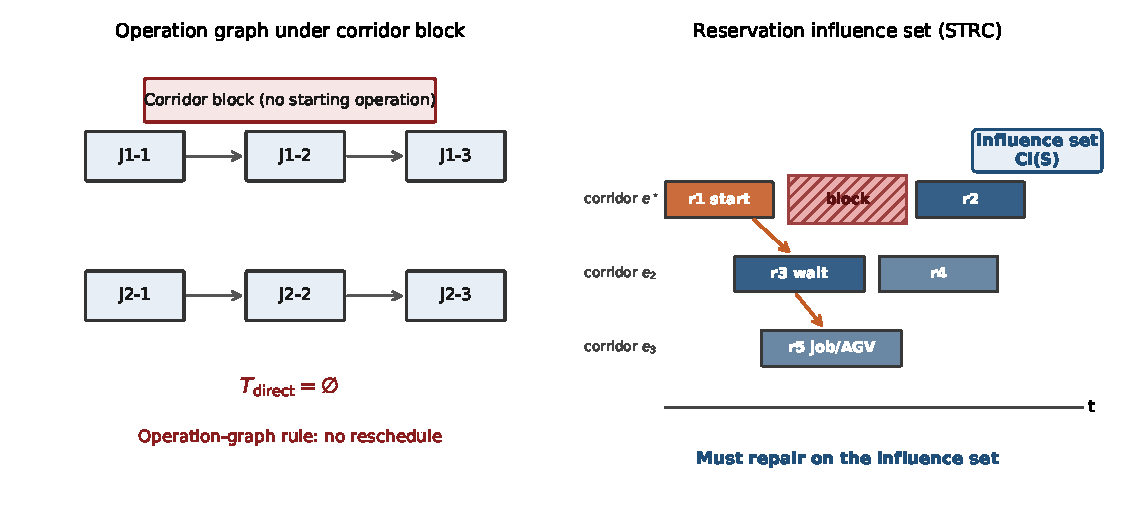
\includegraphics[width=\linewidth]{figures/fig_strc_motivate}
\caption{Motivating illustration. Left: a corridor blockage makes no operation
and no machine unable to run as planned, so the operation-precedence graph has
no operation to start from.
Right: under the same disturbance, the corridor occupancies overlapping the
blockage interval become the starting set and grow into a reservation impact set
along yielding and succession relations.}
\Description{Two panels side by side. The left panel is an operation-precedence
graph in which the corridor blockage renders no operation node unexecutable, so
the set of starting operations is empty. The right panel is the corridor
reservation table at the same instant; the occupancies overlapping the blockage
interval become the starting set, and they spread outwards along yielding edges
and succession edges into a connected region of propagation.}
\label{fig:motivate}
\end{figure}

\subsection{Claims of this paper}

This paper makes three claims.

First, when a flexible job shop uses time-window reservations to guarantee
conflict-free vehicle movement, the post-disturbance rescheduling scope should
be defined on the reservation dependency graph formed by corridor
occupancies and their yielding relations, and not on the operation-precedence
graph alone.

Second, the object the boundary is drawn on is the spatiotemporal reservation
closure (\STRC, Spatiotemporal Reservation Closure), that is, the reservation
impact set: starting from the corridor occupancies that overlap the disturbed
window and are therefore invalidated, every corridor occupancy that must
directly or indirectly be voided and rewritten is brought into the rescheduling
scope along yielding, the next occupancy of the same vehicle, the occupancy of
the next operation of the same job, and the occupancy of the next operation on
the same machine.
Once these dependency relations are given, an occupancy outside the impact set
is no longer a further step from an occupancy inside it along those relations,
so ``which occupancies are to be rewritten'' corresponds to a checkable set
rather than to a search radius fixed by hand.

Third, once the impact set is in hand, the original vehicle is rerouted inside
it while the original occupancies are kept outside it; if a feasible schedule is
still not obtained, the rewritable scope is enlarged in the order same job, same
vehicle, and finally all unfinished occupancies.
For Class-A breakdowns, swapping vehicles and reassigning machines are also
allowed, while the processing sequence still does not change.
These steps serve to put the impact set to work; what this paper claims lies in
how the impact set is delineated, not in whether these repair steps are novel.

The three claims share one position: \textbf{the reservation impact set is a
measurement, not a decision.}
This paper does not use ``who yielded to whom'' to steer a search towards
different assignments or paths---that would be improving the scheduling
decision; once one corridor wait is removed, some other constraint usually
becomes the new bottleneck, so gains in makespan are easily cancelled.
We use the same record of ``who yielded to whom'' to delineate which occupancies
have already been damaged: with the dependency relations given, whether an
occupancy belongs to the impact set depends only on whether it is reachable from
the starting set along those relations, the outcome is uniquely determined, and
it does not change with whichever constraint later becomes the new bottleneck.

This does not amount to claiming that the impact set already contains every
occupancy that must physically be rewritten before feasibility can be restored.
Which dependency edges to draw and which to leave out is a modelling choice;
once the edge set is fixed, the fact that the impact set is closed outwards (no
occupancy inside it has a dependency edge leading outside) is a corollary of the
definition (Proposition~\ref{prop:struct}), not a property proved separately.
Whether the impact set is the smallest set of occupancies needed to restore
feasibility is something this paper does not claim: a smallest set depends on
which repair actions are permitted, and the impact set deliberately does not
commit to any one repair method (Remark~\ref{rem:minimality}).

Relative to global rescheduling, which starts from the original schedule and
searches anew within a time limit, the reservation impact set answers a
different kind of question: when an executable plan must be produced very
quickly, can feasibility be restored and the rewriting confined to the impact
set?
After the repair, the corridor, interval and vehicle of every corridor occupancy
outside the impact set agree with the original plan---a sufficient condition
that holds when the edge set is given and the occupancies outside the set have
been successfully written into the new table as planned
(Proposition~\ref{prop:outside}), not an identity that holds unconditionally.
Relative to global rescheduling that does not rewrite occupancies already
finished at the decision time, the makespan \(C_{\max}\) obtained by bounded
repair is worse, and the fraction of occupancies rewritten is already of the
same order on both sides; its strength is a far shorter algorithm runtime
(milliseconds against seconds).
Algorithm runtime and rewrite fraction should not be explained together, and
Section~\ref{sec:cheap} tests them separately: the short runtime comes from
running path planning once for each transport segment inside the impact set
without restarting a population search, and not from the impact set itself; as
for whether the impact set rewrites fewer occupancies, that cannot be read off
the global-rescheduling comparison above---the two fractions are already
close---and requires a separate comparison in which the rerouting procedure is
identical and the only difference is whether what may be rewritten is the impact
set or every unfinished occupancy.
On the \(6\) instance--seed cells measured, global rescheduling attains the
smaller \(C_{\max}\) at every search time limit, and no case was observed in
which bounded repair was better instead.
The role of bounded repair is therefore not to reduce makespan but to produce an
executable repair within milliseconds.
When the boundary is drawn on the operation-precedence graph, a corridor
blockage finds no affected operation, local rescheduling is never triggered, and
the original schedule stays infeasible.
Starting global rescheduling on the same disturbance would handle it, but with
an algorithm runtime on the order of seconds.
When feasibility must be restored at once, one has to identify the extent of the
damage on the corridor occupancies first, and then choose local recovery steps
that match it.
What this paper solves is that task of identification and recovery, not the task
of finding a rescheduling algorithm with a better makespan.

\subsection{Contributions}
\label{sec:contributions}

The contributions of this paper are as follows.

\begin{enumerate}[leftmargin=1.6em,itemsep=0.4em]
\item \textbf{Identifying a class of damage beyond the reach of the
operation-precedence graph.}
When a schedule uses operation precedence to capture the processing order and
time windows to record corridor occupancies, the off-the-shelf rescheduling
scope is still delineated by affected operations.
Disturbances such as corridor blockage and corridor slowdown change no operation
assignment, the scope delineated by that method is empty, and on that basis no
rescheduling is declared necessary; yet the corridor occupancies overlapping the
disturbed interval have already been invalidated, the original schedule is
infeasible, and the waiting propagates to downstream vehicles along yielding
relations.
The gap is not a missed detection but the fact that the operation-precedence
graph contains no yielding relations among occupancies; were travel times still
taken to be a constant matrix, corridors would not be contendable resources and
damage of this kind could not even be written into the model.

\item \textbf{Defining the rescheduling scope as the reservation impact set.}
Starting from the corridor occupancies overlapping the disturbed window, and
following yielding, the next occupancy of the same vehicle, and the
occupancies of the next operation of the same job and of the same machine, the
records that must directly or indirectly be voided and rewritten are brought
into the rescheduling scope, giving the spatiotemporal reservation closure
(\STRC).
Once the dependency relations are given, whether an occupancy belongs to the
impact set is uniquely determined, and no occupancy inside the set has a
dependency edge leading outside it, so ``which ones to rewrite'' corresponds to
a checkable set rather than a search radius fixed by hand, and does not vary
with how any particular rerouting algorithm is implemented.
The impact set is a measurement, not a scheduling decision: we use ``who
yielded to whom'' to delineate damage, and not to steer a search towards
different assignments or paths.
We do not claim that the impact set is already the smallest set of occupancies
needed to restore feasibility (a smallest set depends on which repair actions
are permitted; Remark~\ref{rem:minimality}).
\emph{The evidence for this layer---whether the impact set stands as an
object---consists of}: under corridor blockage the scope on the
operation-precedence graph is empty while the original schedule is indeed
infeasible, \(\PassMiss\) (Section~\ref{sec:e1}); on Class A the reservation
impact set loses none of the occupancies the operation-precedence graph already
included, \(\PassClosed\) (Section~\ref{sec:e2}); and the differential probe
that ablates the boundary leaks \ProbeLeakPairs.
\emph{Whether this way of drawing the boundary is worth anything in net terms
belongs to another layer}: our evidence there consists of the single RA
comparison (Section~\ref{sec:cheap}), namely how many fewer occupancies are
rewritten relative to ``rewrite every unfinished occupancy''.

\item \textbf{Giving a local recovery that matches this boundary, and keeping
straight where each reading comes from.}
Inside the impact set the original vehicle is rerouted, outside it the original
occupancies are kept; if feasibility is still not attained, the rewritable scope
is enlarged.
These steps serve to put the impact set to work and are not themselves the
methodological contribution of this paper.
Under one and the same corridor network, time-window router and conflict-free
checker, the comparisons show that when the boundary is drawn on the
operation-precedence graph, corridor blockage is recovered on \(\FeasRone\) of
the cells, whereas with the boundary drawn on the reservation impact set it is
recovered on \(\FeasRtwo\); feasibility therefore comes from the object the
boundary is drawn on and not from the quality of the rerouting procedure.
Bounded repair restores feasibility with a runtime on the order of
milliseconds, but its makespan \(C_{\max}\) is worse than that of global
rescheduling, and relaxing the budget produces no crossover
(\(\EfiveCells\) instance--seed cells, no crossing point inside the budget
range measured).
Relative to the comparison that rewrites every unfinished occupancy, runtime
and \(C_{\max}\) barely change, and only the smaller number of rewritten
occupancies can be attributed to the impact set (Section~\ref{sec:cheap}).
In the cross of four disturbance types with two ways of drawing the boundary,
the operation-precedence scope is empty only under corridor blockage and
corridor slowdown, the reservation impact set is non-empty throughout, and under
machine or vehicle breakdown it is no smaller than the operation-precedence
scope.
\end{enumerate}

In the same shop and on the same reservation table, integrated pre-release
scheduling uses the reservation table to build a conflict-free
plan~\cite{vanos2026exact,li2026framework,sun2023integrated}; this paper
uses the reservation table at execution time to locate the extent of the damage.
The two act at different moments and do not substitute for each other.

\subsection{Organization}

Section~\ref{sec:related_work} reviews related work in four classes: how job
shops delineate the rescheduling scope by operations or along the time axis, how
railway rescheduling expresses the order of occupancies on an exclusive
resource, how conflict-free multi-vehicle routing replans locally, and where
flexible job shops with transportation draw the boundary; our own position
follows from this review.
Section~\ref{sec:problem} gives the corridor-reservation setting and the
execution-time recovery problem: the shop, the corridor reservation table and
the operation-precedence graph, the two classes of disturbance, and the
conditions a recovery must satisfy.
Section~\ref{sec:strc} defines the spatiotemporal reservation closure, that is
the reservation impact set, and states its dependency edges and its outward
closedness (Figures~\ref{fig:graphs} and~\ref{fig:closure}).
Section~\ref{sec:repair} explains how the original vehicle is rerouted inside
the impact set while the original occupancies are kept outside it, how the
rewritable scope is enlarged when feasibility is still not attained, and how all
of this compares with global rescheduling (Figure~\ref{fig:framework}).
Section~\ref{sec:experiments} reports feasibility, algorithm runtime, rewrite
fraction and makespan, and uses a case Gantt chart to place the statistical
results on the operation time axis.
Section~\ref{sec:conclusion} concludes and discusses limitations and future
work.

%% =====================================================================
\section{Related work}
\label{sec:related_work}
%% =====================================================================

%% Related work is reviewed by problem type; no "four-layer positioning" is
%% attempted.  Older references are kept as citation clusters and the narrative
%% is carried by recent work.

One basic question in dynamic scheduling is: once a disturbance has occurred, on
what object is the rescheduling scope drawn, that is, what is changed and what
is left alone.
The existing literature draws this scope on different objects---operations or the
time axis, the order of occupancies on an exclusive resource, the affected
vehicles, and the set of operations in a flexible job shop with transportation.
Below we review, for each of these four classes, what it does and what it does
not yet cover, and summarize the review in Table~\ref{tab:position}.

\subsection{Local rescheduling in job shops}
\label{sec:rw_aor}

For operation-level events such as machine breakdown and order insertion,
delineating the rescheduling scope by affected operations is still in use in
dynamic scheduling with AGVs.
Zhang et al.~\cite{zhang2023energy} treat machine breakdown and order insertion
and take the recovery scope to be the operations not yet processed after the
breakdown; Tang et al.~\cite{tang2026dynamic} sort operations and delivery tasks
into retained, continued and reconstructed according to how the disturbance
affects them, and place complete rescheduling, partial rescheduling and right
shift side by side, noting that a right shift preserves stability at the cost of
optimization room.
The original sentences on which the paraphrases of this and the next subsection
rest are collected in Table~\ref{tab:refcheck}.
The practice traces back to affected-operations rescheduling
(AOR)~\cite{abumaizar1997rescheduling,subramaniam2003maor}: only the operations
directly or indirectly touched by the disturbance are rearranged.
Drawing the boundary along the time axis, and enlarging the scope after a
failure, have likewise been studied, including
match-up~\cite{akturk1999matchup} and Local Rescheduling with incrementally
widened time windows~\cite{kuster2007local}.
A right shift, by contrast, decides nothing about who is affected and simply
pushes the unfinished part back as a whole.
Rolling-horizon and decomposition methods trade off scale against
quality~\cite{zeitrag2025novel,zhao2019decomposition}; for surveys
see~\cite{vieira2003rescheduling,ouelhadj2009survey}.

This body of work shows that delineating a scope and then rescheduling locally is
not a new problem, provided that the disturbance acts on operations in the first
place.
Once a disturbance only makes a corridor impassable without changing any
assignment, the scope delineated by that method can be empty while the original
schedule is already infeasible.

\subsection{The order of occupancies on an exclusive resource}
\label{sec:rw_ag}

``Who occupies the same exclusive resource first'' has been modelled as a graph
and studied systematically in railway rescheduling.
The alternative graph of Mascis and Pacciarelli~\cite{mascis2002alternative}
generalizes the disjunctive graph as follows: a vertex is the occupancy of a
block section by a job, fixed arcs express the order along a route, and a pair of
alternative arcs expresses who passes through that section first.
D'Ariano et al.~\cite{dariano2007branch} use the model for real-time train
rescheduling, recomputing a conflict-free timetable after a disturbance while
staying as close as possible to the original plan.
Yielding on a shared corridor and an alternative arc express the same kind of
ordering.

What differs from the present paper is the use made of it.
For every point of contention the alternative graph offers two mutually
exclusive arcs (either A passes first, or B does), and scheduling consists in
selecting one of them: after the selection the graph must contain no
positive-weight cycle for the timetable to be feasible, and the objective is to
be made as good as possible---the order of occupancies is therefore a decision
variable.
In this paper the plan has already been produced, who passes through which
corridor first has already been fixed, and the order is no longer selected;
those given yielding and succession relations are used only to bring the
original corridor occupancies that must be voided after a disturbance into the
rescheduling scope.
Furthermore, the railway model treats a block section as a machine, so that
operations and occupancies live on one and the same graph and an unavailable
section simply is an operation-level event; the situation of ``a scope drawn on
the operation-precedence graph and therefore blind to corridor blockage'' does
not arise.
In a flexible job shop, processing and corridor occupancy are two distinct
families of objects, and the off-the-shelf AOR boundary cannot make use of this
order of occupancies.

\subsection{Local replanning in conflict-free multi-vehicle routing}
\label{sec:rw_mapf}

In multi-agent path finding, rescheduling only the affected agents while
treating the rest as dynamic obstacles is already standard practice.
\v{S}vancara et al.~\cite{svancara2019online} give Replan All, Replan Single and
Replan Affected for online MAPF and use online independence detection to
determine the affected set; Malka et al.~\cite{malka2024online} likewise replan
only for the vehicles affected by observed changes when the map is inaccurate.
Conflict-free path planning treats spatiotemporal occupancy as a first-class
constraint, but the origins and destinations are usually given
externally~\cite{zhang2024guidance}.

This line of work has already made ``change only the affected agents, keep the
original plan for the rest'' into a standard mechanism, and we do not claim it as
a contribution.
A second difference from our setting is that such work has only vehicle origins
and destinations, with no job--operation--machine assignment, so ``the
rescheduling scope is delineated on the operation-precedence graph and corridor
blockage is missed because no affected operation can be found'' cannot arise.
As to how the affected set is obtained, MAPF finds the affected vehicles by
independence detection, which yields the output of a detection algorithm and
therefore varies with the implementation and the stopping condition.
The reservation impact set given here is different: once the dependency edges
are given, whether an occupancy belongs to the set depends only on whether it is
reachable from the starting set along those edges, independently of which
rerouting algorithm is used afterwards (Section~\ref{sec:containment}).

\subsection{Flexible job shop scheduling with transportation}
\label{sec:rw_position}

Flexible job shop scheduling with transportation vehicles has been surveyed
systematically~\cite{xin2025review}.
Recent combinatorial-optimization work still commonly takes travel time to be a
constant matrix indexed by pairs of locations, and develops constraint
programming, metaheuristics and knowledge-guided search on top of
it~\cite{meng2025cp,qin2026knowledge,fu2025integrated}.
Under that convention vehicles do not contend for the same corridor, corridor
blockage has no corresponding object in the model, and it cannot be tested.

Once corridor occupancies are recorded by time windows, processing order and
corridor occupancy enter the model together.
Congestion-aware dispatching can select a vehicle using an indirect measure such
as local density, without changing the machine
assignment~\cite{kim2026congestion}.
Work that genuinely brings flexible assignment and conflict-free transportation
together is comparatively scarce: van Os and Basten~\cite{vanos2026exact}
formalize flexible job shop scheduling with conflict-free transportation
constraints and, with a decomposition method, attain provable optimality on most
benchmark instances, optimality not being guaranteed on a few because of a time
limit; a two-stage scheme first fixes production and then resolves vehicle
conflicts~\cite{sun2023integrated}; and there is also a framework in which a
learning layer schedules production, a routing layer resolves conflicts, and the
two are connected by limited feedback~\cite{li2026framework}.
What all of these answer, however, is how to produce a feasible and good-quality
conflict-free schedule before release.

To the authors' knowledge, no work has yet taken both a corridor reservation
table and execution-time disturbance response into account.
This sentence is a bounded one: we do not claim to have exhausted the
literature, and therefore do not state it as a universal negative.
What can be checked paper by paper is that in the work cited in this section the
two conditions never appear together---those with a reservation table exclude
execution-time breakdowns, and those that handle execution-time disturbances
have no reservation table.
The following two points rest on the modelling assumptions stated in the
originals (the sentences are reproduced verbatim in Table~\ref{tab:refcheck}):
Zhang et al.~\cite{zhang2023energy} state in their modelling assumptions that
collisions between AGVs are ignored; Sun et al.~\cite{sun2023integrated} resolve
vehicle conflicts with a time-window Dijkstra search, yet state in their
assumptions that vehicle charging and breakdowns are not considered and that
vehicles are always available, and list equipment maintenance and breakdowns as
future research.

The gap, then, is not that some existing paper drew the boundary in the wrong
place, but that in the work listed above the two conditions were never in place
at once: an operation-level boundary holds, often because there is no corridor
reservation; and settings that do have a reservation table exclude
execution-time disturbances.
Once both are present, the only off-the-shelf option is to delineate the scope by
affected operations, and for a corridor blockage that changes no operation
assignment this returns an empty scope (\PassMiss\ as measured in
Section~\ref{sec:e1}).
This is the situation the present paper addresses.
It should be noted that \textbf{the counterexample itself does not depend on the
gap statement above holding}: even if existing work did incorporate both
conditions, the readings of Section~\ref{sec:e1} would still stand, and what
would be affected is our novelty claim, not its correctness.

The gap assessment above and the positioning in Section~\ref{sec:rw_aor} both
rest on paraphrases of other people's work, and a paraphrase can distort.
So that a reader need not fetch the originals to check, the sentences on which
these paraphrases rest are listed in Table~\ref{tab:refcheck}.
The immediate reason for the list is that one of them failed the check: the
conclusion of van Os and Basten~\cite{vanos2026exact} was originally paraphrased
here as ``a benchmark with provable optimality obtained by a decomposition
method'', whereas the original confines this to most instances, optimality not
being guaranteed on a few because of time boxing.
The direction of the deviation is worth recording---it strengthened the
conclusion on behalf of the cited work, and what was strengthened happened to be
the very baseline this paper compares against.

\begin{table}[t]
\centering
\caption{Paraphrases on which the positioning depends, against the cited
originals. The five paraphrases \emph{from which the gap is drawn} are listed,
each with the original sentence of the cited work, so that the reader can judge
the fidelity of the paraphrase without fetching the original.
Row 4 is a paraphrase already corrected: the earlier wording was stronger than
the original and has now been narrowed to match it (see the body).}
\label{tab:refcheck}
\footnotesize
\begin{tabular}{@{}p{0.23\linewidth}p{0.55\linewidth}p{0.14\linewidth}@{}}
\toprule
\textbf{Our paraphrase} & \textbf{Cited original} & \textbf{Location in the original} \\
\midrule
The recovery scope of Zhang et al.~\cite{zhang2023energy} is the operations not
yet processed after the breakdown &
\emph{``Rearrange the unprocessed operations of current scheme considering the limit of
machine breakdown''} &
Rescheduling procedure \\
\addlinespace
Zhang et al.~\cite{zhang2023energy} state in their modelling assumptions that
collisions between AGVs are ignored &
\emph{``The collision of AGVs are ignored.''} &
Modelling assumption (7) \\
\addlinespace
Tang et al.~\cite{tang2026dynamic} sort operations and delivery tasks into
retained, continued and reconstructed according to how the disturbance affects
them &
\emph{``an event-driven partial rescheduling strategy is proposed, in which the disrupted
operations and delivery tasks are classified into three categories: retained, continued,
and reconstructed''} &
Abstract \\
\addlinespace
van Os and Basten~\cite{vanos2026exact} attain provable optimality on most
benchmark instances, optimality not being guaranteed on a few because of a time
limit &
\emph{``For most benchmark instances, our LBBD-based approach finds optimal makespan
values. Because of time boxing, only in a few cases, the optimality of the found solution
cannot be guaranteed.''} &
Abstract \\
\addlinespace
Sun et al.~\cite{sun2023integrated} assume that vehicles are always available
and do not consider breakdowns or charging, and list equipment maintenance and
breakdowns as future research &
\emph{``It does not consider the charging problem and fault problem of the AGVs, and AGVs
are always available''}; \emph{``Breakdowns and charging problems are not taken into
account.''}; \emph{``Future research will investigate the impact of equipment maintenance
and breakdowns on production scheduling''} &
Assumption list, future work \\
\bottomrule
\end{tabular}
\end{table}

\subsection{Our position}
\label{sec:rw_claim}

\begin{table*}[t]
\centering
\caption{Related work classified by \emph{the object the boundary is drawn on}:
on which kind of object each class of work defines ``what needs to be
rewritten'' after a disturbance.
``Boundary drawn on'' is the object the rescheduling scope is attached to;
``operation-precedence graph?'' also answers whether that graph shares a graph
with the occupancies; the bold entry in the last row is the class this paper
belongs to.}
\label{tab:position}
\small
\begin{tabular}{@{}p{0.16\linewidth}p{0.22\linewidth}p{0.14\linewidth}p{0.14\linewidth}p{0.24\linewidth}@{}}
\toprule
\textbf{Class} & \textbf{Representative work} & \textbf{Boundary drawn on} & \textbf{Operation-precedence graph?} & \textbf{Relation to this paper} \\
\midrule
Local rescheduling in job shops &
AOR~\cite{abumaizar1997rescheduling,subramaniam2003maor};
match-up~\cite{akturk1999matchup};
LRS~\cite{kuster2007local};
dynamic scheduling with AGVs~\cite{zhang2023energy,tang2026dynamic} &
Operations / time windows & Yes &
Reproduced later as the operation-level boundary and the right-shift comparisons \\
\addlinespace[2pt]
Order of occupancies on an exclusive resource &
alternative graph~\cite{mascis2002alternative};
real-time railway rescheduling~\cite{dariano2007branch} &
Occupancy of a block section & Yes, on the same graph as the occupancies &
Yielding relations are of the same kind; railways use them to choose the order of
vehicles, whereas we use the given order to delineate the occupancies that need
rewriting \\
\addlinespace[2pt]
Conflict-free multi-vehicle routing &
Online MAPF~\cite{svancara2019online,malka2024online};
LMAPF~\cite{zhang2024guidance} &
Affected vehicles & No &
Rerouting inside the set and keeping the plan outside it is already standard
practice \\
\addlinespace[2pt]
Flexible job shop with transportation &
constant matrix~\cite{xin2025review,meng2025cp,qin2026knowledge,fu2025integrated};
integrated scheduling~\cite{vanos2026exact,sun2023integrated,li2026framework} &
Set of operations & Yes; a reservation table and execution-time disturbances
never appear together &
\textbf{Our position} \\
\bottomrule
\end{tabular}
\end{table*}

In summary, in a flexible job shop with conflict-free AGV routing, the schedule
uses operation precedence to capture the processing order and time windows to
record corridor occupancies.
The situation identified as a gap in the previous section then arises:
disturbances such as corridor blockage do not make operations unexecutable and
the original assignment remains valid, yet the corridor occupancies overlapping
the disturbed interval have been invalidated and the original schedule is
infeasible.
The comparison arm that delineates the scope on the operation-precedence graph,
used later on, reproduces the practice of Section~\ref{sec:rw_aor}.
This paper argues for moving the rescheduling scope onto the corridor
occupancies together with their yielding and succession relations, which yields a
reservation impact set uniquely determined by those relations.

%% =====================================================================
\section{The corridor-reservation setting and the execution-time recovery problem}
\label{sec:problem}
%% =====================================================================

\subsection{System setting and notation}
\label{sec:system_brief}

The problem setting follows the flexible job shop with conflict-free
transportation constraints~\cite{vanos2026exact}.
This section states once and for all the objects used later.
A feasible schedule \(\mathcal{S}^0\) is regarded as given input: how it was
found by search at \(t=0\) has no bearing on how the occupancies that must be
rewritten are delineated later.

\subsubsection{The shop and the four groups of decisions}
\label{sec:shop}

The routing graph of the shop \(G=(V,E)\) is strongly connected.
Robotic arms occupy fixed nodes \(\mathrm{loc}(m)\), and \(v_0\in V\) is the
load/unload station.
There are \(n\) jobs, a machine set \(M\), and a homogeneous single-load fleet
\(K=\{1,\ldots,N_A\}\).
Job \(j\) has a fixed operation chain \(O_{j1}\to\cdots\to O_{jn_j}\); the set of
eligible machines of operation \(O_{ji}\) is \(\Omega_{ji}\subseteq M\), and its
processing time on machine \(m\) is \(t^P_{jim}\).
A complete schedule fixes four groups of decisions at once:
(i)~the machine assignment \(x\) of every operation;
(ii)~the operation sequence \(\pi\) on every machine;
(iii)~the vehicle assignment \(y\) of every transport;
(iv)~a conflict-free path on \(G\) for every vehicle movement.
We write
\[
\mathcal{S}=(x,\,\pi,\,y,\,R),
\]
where the reservation table \(R\) is the explicit record of group (iv), defined
below.

Transport tasks are \emph{induced} by the assignment rather than given as input:
a transport arises only when two consecutive operations are not at the same
node.
A transport splits into two segments---an empty travel to pick up and a loaded
travel to deliver---each with its own task label \(u\) (the empty and the loaded
segment of \(O_{ji}\), for instance, are two separate records).
Loading and unloading are instantaneous: the loaded segment departs at the later
of the arrival of the empty segment and the readiness of the job, and the
delivery instant is at once the instant at which the machine may start and the
vehicle may take a new task.
Which occupancies may be rewritten later, which keep the original plan, and how
rerouting proceeds are all handled at the granularity of a segment, not of a
whole operation.

\subsubsection{Corridor reservations and conflict freedom}
\label{sec:reservation}

Every corridor \(e\in E\) is an exclusive resource with known traversal time
\(\tau_e\); the two directions share one occupancy, so at most one vehicle
occupies \(e\) at any instant, and head-on conflicts and same-direction
overtaking are both excluded.
Occupancies are half-open intervals: a second vehicle may enter exactly at the
right endpoint.
Nodes carry ample berths, so waiting happens at nodes and is always permitted.
A reservation is recorded as
\[
r=(e,\,[t^s,t^e),\,k,\,u)\in R,
\]
that is, vehicle \(k\) occupies corridor \(e\) during \([t^s,t^e)\) as part of
transport segment \(u\).
Any two distinct occupancies of the same corridor must satisfy
\([t^s,t^e)\cap[t^{s\prime},t^{e\prime})=\varnothing\).
A path is written only into the time windows that \(R\) reports as free, so
conflict freedom is constructed rather than repaired after the fact.

Time-window routing is the primitive shared by the rerouting below and by every
comparison method: given an origin and destination, an earliest departure time
and the current \(R\), it returns a path disjoint from the existing occupancies
together with the entry time at each corridor.
The implementation uses a time-window Dijkstra search~\cite{sun2023integrated};
this paper does not modify the primitive and changes only \emph{which} transport
segments are handed to the router.
Unlike van Os, who reserves nodes, and Lyu, who adds node
capacities~\cite{vanos2026exact,lyu2019approach}, we reserve edges;
Section~\ref{sec:limitations} explains the resulting restriction on which
instances can be used.

\subsubsection{The operation-precedence graph and the reservation dependency graph}
\label{sec:two_graphs}

The operation-precedence graph \(G_T=(T_T,E_T)\) (also called the task graph in
the literature, whence the subscript \(T\)) has operations as vertices and, as
edges, the precedence within a job and the precedence on a machine; it
\emph{does not contain} yielding relations among corridor occupancies.
The reservation dependency graph \(G_R=(R,E_R)\) has the occupancies in \(R\) as
vertices, and as edges the dependencies induced by yielding, the same vehicle,
the same job and the same machine (Definition~\ref{def:dep}).
The vertex sets of the two graphs are disjoint: one is processing, the other is
travel.
There is therefore a class of disturbance that changes only corridor time
windows and no operation parameter---delineating the scope on \(G_T\) finds no
operation to start from, whereas delineating it on \(G_R\) yields a non-empty set
of starting occupancies, and the original schedule is already infeasible.
Figure~\ref{fig:graphs} contrasts the two graphs, Figure~\ref{fig:motivate} shows
the consequence under a corridor blockage, and Table~\ref{tab:notation}
summarizes the notation used in this section and later.

\begin{figure}[t]
\centering
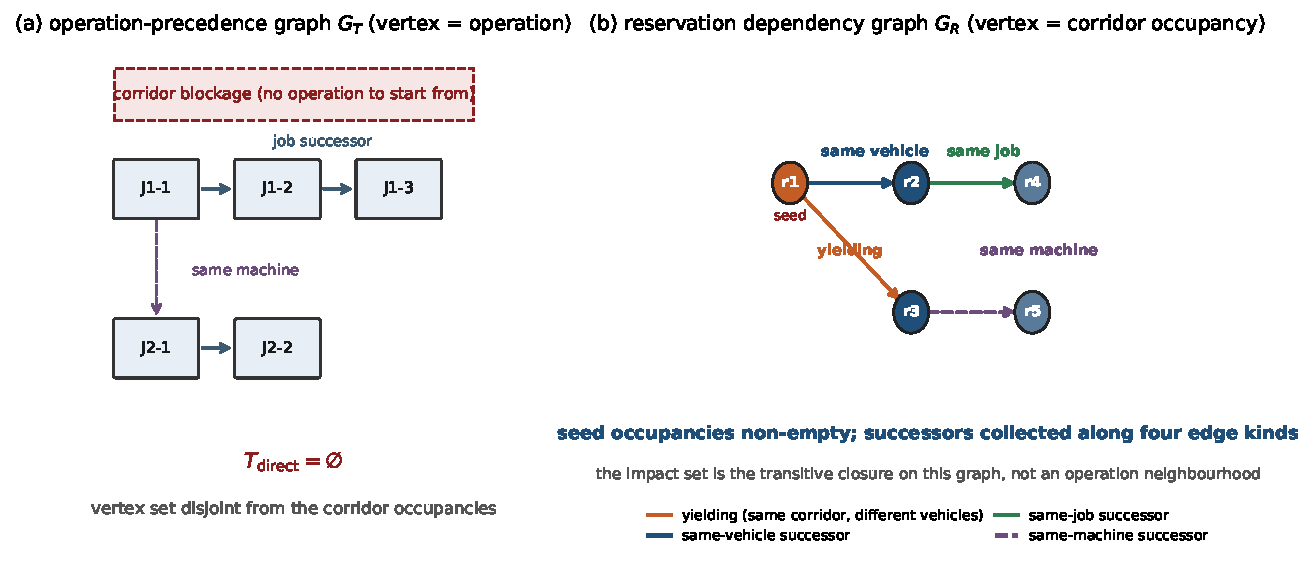
\includegraphics[width=\linewidth]{figures/fig_strc_graphs}
\caption{The vertex sets of the two graphs are disjoint (schematic
construction).
(a)~The operation-precedence graph \(G_T\), whose vertices are operations; a
corridor blockage finds no operation to start from.
(b)~The reservation dependency graph \(G_R\), whose vertices are corridor
occupancies; starting from the occupancies overlapping the blockage window, the
downstream occupancies are collected along four kinds of dependency edge
(yielding, same vehicle, same job, same machine; Definition~\ref{def:dep}).}
\Description{Two panels side by side. The left panel is an operation-precedence
graph in which job successors and same-machine successors connect boxes
representing operations; a dashed box at the top marks the corridor blockage,
which lands on none of the boxes.
The right panel is the reservation dependency graph, in which five circular
vertices represent corridor occupancies and four arrows in different colours are
labelled yielding, same vehicle, same job and same machine.}
\label{fig:graphs}
\end{figure}

\begin{table}[t]
\centering
\caption{Notation used throughout the paper}
\label{tab:notation}
\small
\begin{tabular}{@{}ll@{}}
\toprule
\textbf{Symbol} & \textbf{Meaning} \\
\midrule
\(G=(V,E)\), \(\tau_e\) & corridor network; traversal time of corridor \(e\) \\
\(v_0\), \(\mathrm{loc}(m)\) & load/unload station; node of robotic arm \(m\) \\
\(x,\pi,y\) & machine assignment, operation sequence, vehicle assignment \\
\(R\), \(r=(e,[t^s,t^e),k,u)\) & reservation table; one half-open occupancy (vehicle \(k\), segment label \(u\)) \\
\(G_T\) / \(G_R\) & operation-precedence graph / reservation dependency graph \\
\(\mathcal{S}^0,\mathcal{S}'\) & schedule before the disturbance, schedule after recovery \\
\(\mathcal{D},\,t_{\mathrm{now}}\) & disturbance event; instant at which it occurs (the decision time) \\
\(T_{\mathrm{direct}},\,T_{\mathrm{impact}}\) & operations directly disturbed on the operation-precedence graph / scope collected within \(\theta\) steps \\
\(\mathrm{Seeds}(\mathcal{D})\), \(U\) & occupancies used as starting points; set of occupancies allowed to be rewritten \\
\(\mathrm{Cl}(\cdot)\) & reservation impact set (\STRC) \\
\(\varphi\) & fraction of future operations disturbed (scale sweep) \\
\bottomrule
\end{tabular}
\end{table}

\subsection{Execution-time assumptions}
\label{sec:assumptions}

The execution-time conventions and the physical setting are as follows.
A1--A4 are shared by every comparison method, so that the readings can be
attributed to how the rescheduling scope is delineated rather than to a
difference of models; A5 constrains our method only, the global-rescheduling
comparison being allowed a wider set of actions (see the last sentence of that
item):

\begin{enumerate}[label=\textbf{A\arabic*.},leftmargin=*,topsep=2pt,itemsep=2pt]
\item \textbf{The initial schedule is feasible.} \(\mathcal{S}^0\) passes the
conflict-free check before the disturbance, and the reservation table agrees with
the operation timetable.
\item \textbf{Finished occupancies are not revisited.} Only unfinished
occupancies with \(t_{\mathrm{end}}>t_{\mathrm{now}}\) and unfinished operations
may be rewritten; the fields of an occupancy with
\(t_{\mathrm{end}}\le t_{\mathrm{now}}\) may not.
\item \textbf{A single, fully observed disturbance.} The disturbance is observed
in full at \(t_{\mathrm{now}}\) and does not overlap with another; disturbance
streams, prediction error and rolling response are outside the scope of this
paper.
\item \textbf{Exclusive corridors, ample buffers, a homogeneous single-load
fleet.} Corridors remain exclusive half-open resources, and a blockage is
injected into the routing layer as an additional occupancy (or a no-entry
window).
Finite buffers, charging, acceleration and deceleration, and loading times are
not modelled; every vehicle stands empty at \(v_0\) when the plan begins.
\item \textbf{Permitted recovery actions.} A Class-B disturbance keeps the
original machine assignment \(x\) and sequence \(\pi\) and only reroutes; on
failure the set of rewritable occupancies is enlarged.
A Class-A breakdown permits two further actions: a vehicle breakdown removes the
failed vehicle from the fleet and swaps in another; a robotic-arm breakdown
reassigns the unfinished operations to other eligible machines.
The sequence \(\pi\) never changes and no search is restarted.
The global-rescheduling comparison in the experiments may change \(x\) and
\(\pi\) (Section~\ref{sec:vs_r0}).
\end{enumerate}

\subsection{A dichotomy of disturbances}
\label{sec:disturbance_classes}

\begin{definition}[Class-A and Class-B disturbances]
\label{def:ab}
A disturbance is called \textbf{Class A} if it directly invalidates the
assignment or the \emph{executability} of some operations (robotic-arm
breakdown, marked deviation in processing time, order insertion, vehicle
breakdown, and so on); it is called \textbf{Class B} if it only makes some
corridor time windows unavailable without making any operation unexecutable
(corridor blockage, corridor slowdown, and so on).
\end{definition}

\begin{remark}[Why vehicle breakdown is Class A]
\label{rem:agv_class}
A vehicle breakdown changes the machine assignment of no operation, and at first
sight belongs with corridor blockage.
The criterion of Definition~\ref{def:ab}, however, is \emph{executability} and
not assignment: once a vehicle has broken down, the operations it was carrying
cannot start under the original plan, so through the map ``vehicle \(\to\) the
operations it carries'' the operation-precedence graph still has operations to
start from.
This classification places vehicle breakdown on the side where an
operation-level boundary does return a non-empty scope.
Those starting operations are non-empty only if the rescheduling method
maintains the vehicle--task map; if the method tracks operations and machines
only (as is common in implementations of AOR), a vehicle breakdown likewise
yields an empty scope.
This paper does not rest its argument on that point:
Section~\ref{sec:e6} reports the Class-A readings under the stronger convention
in which the map is maintained.
\end{remark}

\begin{definition}[The direct set and the impact region on the operation-precedence graph]
\label{def:task_impact}
For a disturbance \(\mathcal{D}\), let \(T_{\mathrm{direct}}(\mathcal{D})\) be
the set of operations that cannot run as planned because of a machine breakdown,
a vehicle breakdown or an invalidated operation.
For a Class-B corridor disturbance we set \(T_{\mathrm{direct}}=\varnothing\) by
convention.
Starting from \(T_{\mathrm{direct}}\) on \(G_T\) and collecting the operations at
depth at most \(\theta\) along job successors and same-machine successors gives
\(T_{\mathrm{impact}}(\mathcal{D},\theta)\).
\end{definition}

\begin{definition}[Occupancies used as starting points]
\label{def:seeds}
The starting set \(\mathrm{Seeds}(\mathcal{D})\subseteq R\) is given per
disturbance type and always contains only occupancies with
\(r.t^e>t_{\mathrm{now}}\).
\begin{enumerate}[label=(\alph*),leftmargin=1.6em,itemsep=0.15em]
\item \textbf{Corridor blockage / slowdown} \(\mathcal{D}=(e,[t_a,t_b))\):
\(\{\,r:\ r.e=e,\ [r.t^s,r.t^e)\cap[t_a,t_b)\neq\varnothing\,\}\).
For several brief blockages one takes the union of the starting occupancies of
the individual windows.
The two disturbance types share this rule for starting points (the original
schedule was written with the unscaled \(\tau\), so every occupancy overlapping
the window has already been invalidated), and therefore yield the same
reservation impact set when the occupancies to be rewritten are
delineated---Section~\ref{sec:e6} uses this to explain why their boundary
readings are not counted as two independent validations.
At the rerouting stage the two are already separated: a slowdown scales progress
only on the portion overlapping the window, and is no longer written as a
prohibition on the whole segment, nor is an intersecting traversal multiplied by
the factor over its whole length.
\item \textbf{Vehicle breakdown} \(\mathcal{D}=(k)\): every occupancy of that
vehicle after \(t_{\mathrm{now}}\), \(\{\,r:\ r.k=k\,\}\).
\item \textbf{Robotic-arm breakdown} \(\mathcal{D}=(m,F)\), with \(F\) the
operations on that machine not yet finished: for each job take the smallest
operation index \(i_{\min}(j)\) in \(F\), and let the starting occupancies be all
unfinished occupancies of each job from that operation onwards (inclusive).
The reason for taking the whole job suffix rather than the operation itself is
that the inbound transport may already have finished before
\(t_{\mathrm{now}}\); taking the operation alone would make the reservation
impact set shorter than the impact region on the operation-precedence graph, and
the comparison would be unfair.
\end{enumerate}
\end{definition}

\begin{prop}[On Class B the operation-precedence graph returns an empty scope]
\label{prop:miss}
Let \(\mathcal{D}\) be a corridor blockage. Under the Class-B convention of
Definition~\ref{def:task_impact} we have
\(T_{\mathrm{direct}}(\mathcal{D})=\varnothing\) and hence
\(T_{\mathrm{impact}}(\mathcal{D},\theta)=\varnothing\) for every finite
\(\theta\ge 0\).
If in addition \(\mathrm{Seeds}(\mathcal{D})\neq\varnothing\), then
\(\mathcal{S}^0\) is infeasible under \(\mathcal{D}\).
\end{prop}

\begin{proof}
A corridor blockage makes corridor time windows unavailable without making any
operation unexecutable, and is therefore Class B by Definition~\ref{def:ab}.
This step uses two premises: the blockage window \([t_a,t_b)\) is finite, and by
Assumption A4 buffers are ample so that vehicles can pass outside the window;
hence even if the network is cut during the blockage, no operation becomes
unexecutable and it is merely delayed.
If the blockage were indefinite, or the buffers insufficient to support the
waiting, the disturbance would be Class A by Definition~\ref{def:ab} and would
lie outside the scope of this proposition.
Being Class B, it follows from the Class-B convention of
Definition~\ref{def:task_impact} that \(T_{\mathrm{direct}}=\varnothing\).
The starting set of the \(\theta\)-step collection is empty, so
\(T_{\mathrm{impact}}=\varnothing\).
If some \(r\in\mathrm{Seeds}(\mathcal{D})\) exists, its occupancy interval
intersects the no-entry window.
Interpreting \(\mathcal{D}\) as a compulsory occupancy of that corridor, \(r\)
and the no-entry window overlap in time on the same exclusive resource, which
violates the half-open conflict-free condition (corridor exclusivity in
Assumption A4); hence \(\mathcal{S}^0\) is infeasible.
\end{proof}

Proposition~\ref{prop:miss} is a counterexample at the level of the problem.
The first half follows directly from the Class-B convention of
Definition~\ref{def:task_impact} (the operation-precedence graph contains, by
definition, no yielding relations among corridor occupancies and therefore
cannot reach a corridor blockage); what is non-trivial is the second half---once
the starting occupancies are non-empty, the original schedule is already
infeasible, and so ``an empty scope on the operation-precedence graph
\(\Rightarrow\) no rescheduling needed'' fails in a setting where corridors are
reserved by time windows.
The counterexample depends on no repair algorithm;
Section~\ref{sec:experiments} reports the sizes of the instances.

\subsection{The recovery problem}
\label{sec:recovery_problem}

\begin{problem}[Bounded repair with the scope delineated on the reservation table]
\label{prob:recovery}
Given a feasible schedule \(\mathcal{S}^0\), a disturbance \(\mathcal{D}\) and an
instant \(t_{\mathrm{now}}\), find \(\mathcal{S}'\) such that:
(i)~\(\mathcal{S}'\) passes the conflict-free check under \(\mathcal{D}\);
(ii)~the corridor, interval and vehicle of every occupancy not brought into the
rewritable scope agree with \(\mathcal{S}^0\) as far as possible;
(iii)~the algorithm runtime respects a budget.
The secondary objective is the makespan \(C_{\max}(\mathcal{S}')\).
\end{problem}

Solving it splits into two steps: first delineate the set of occupancies allowed
to be rewritten, \(U\subseteq R\); then reroute only the transports inside
\(U\), keeping the original plan for the occupancies outside it.
We give \(U\) as \(\mathrm{Cl}(\mathrm{Seeds})\); the comparison arm instead
induces a subset of reservations from the impact region on the
operation-precedence graph.

%% =====================================================================
\section{The spatiotemporal reservation closure}
\label{sec:strc}
%% =====================================================================

This section produces nothing but the set \(U\) of occupancies allowed to be
rewritten: given the reservation table \(R\) and the set of starting occupancies
\(\mathrm{Seeds}(\mathcal{D})\) (Definition~\ref{def:seeds}), a dependency graph
is built on the occupancies and its transitive closure taken, yielding
\(U=\mathrm{Cl}(\mathrm{Seeds})\); how rerouting proceeds on \(U\) belongs to
Section~\ref{sec:repair}.

\subsection{Reservation dependency edges}
\label{sec:closure_def}

\begin{definition}[Reservation dependency graph]
\label{def:dep}
The vertices are the corridor occupancies in \(R\). A directed edge
\(r\to r'\) means ``the invalidation of \(r\) may force \(r'\) to be rerouted'',
and comprises:
\begin{enumerate}[leftmargin=1.4em,itemsep=0.15em]
\item \textbf{Yield edge:} same corridor, different vehicles, overlapping in time
\emph{or abutting as half-open intervals} (\(r.t^e=r'.t^s\)), directed from the
earlier entrant to the later one; abutment is legal under the exclusivity
semantics, but if the former is delayed the latter must yield;
\item \textbf{Same-vehicle successor:} two occupancies of the same vehicle that
are adjacent in time;
\item \textbf{Same-job successor:} an occupancy of operation \(i\) of a job
points to an occupancy of operation \(i+1\);
\item \textbf{Same-machine successor:} an edge between the occupancies induced by
two operations adjacent on the time axis of the same machine.
\end{enumerate}
This yields \(G_R=(R,E_R)\).
The four kinds of edge are illustrated in Figure~\ref{fig:graphs}(b).
A same-job successor connects the occupancies induced by consecutive operations,
and a same-machine successor connects the occupancies induced by two operations
adjacent on the time axis of one machine; both have segments as endpoints,
matching the granularity of Section~\ref{sec:shop}.
The four kinds of edge answer one question only: after \(r\) has been rewritten,
may \(r'\) have to be rewritten too. They do not attempt to capture every
physical coupling; the edge set is itself a modelling choice, its completeness is
tested by the differential probe of Section~\ref{sec:e3}, and the corresponding
qualifications appear in Section~\ref{sec:containment}.
\end{definition}

\begin{definition}[\STRC{}]
\label{def:strc}
For a set of starting occupancies \(S\subseteq R\), a horizon \(H\) and an
instant \(t_{\mathrm{now}}\), write the occupancies that have not finished at the
decision time and that start before the horizon as
\[
R^{\circ}=\bigl\{\,r\in R:\ r.t^e>t_{\mathrm{now}},\ r.t^s<H\,\bigr\},
\]
and let \(G_R^\circ\) be the subgraph of \(G_R\) induced on \(R^{\circ}\).
The reservation impact set (the spatiotemporal reservation closure) is defined as
\[
\mathrm{Cl}(S)
=\bigl\{\,v\in R^{\circ}:\
\exists\,s\in S\cap R^{\circ}\ \text{such that}\ s\!\to^*\!v\ \text{in}\ G_R^\circ\,\bigr\},
\]
that is, every unfinished occupancy reachable along out-edges from an unfinished
starting occupancy (the starting occupancies themselves included).
Every experiment in this paper takes \(H=C_{\max}(\mathcal{S}^0)+1\), so that
\(r.t^s<H\) holds for every occupancy of \(\mathcal{S}^0\) and the horizon
performs no filtering; \(H\) is retained only so that the definition remains
usable with a rolling horizon.
Representing \(G_R^\circ\) by adjacency lists (writing its edge set as
\(E_R^{\circ}\)), the closure can be computed with a queue in
\(O(|R^{\circ}|+|E_R^{\circ}|)\) time; this bound is not timed separately, since
delineating the boundary is only one component of the millisecond-level readings
of Section~\ref{sec:cheap}.
\end{definition}

Figure~\ref{fig:closure} illustrates: (a) the blockage window and the occupancies
used as starting points; (b) the dependency edges and the shell of the
reservation impact set---an occupancy outside the set is not an out-edge successor
of one inside it (Proposition~\ref{prop:struct}).

\begin{figure}[t]
\centering
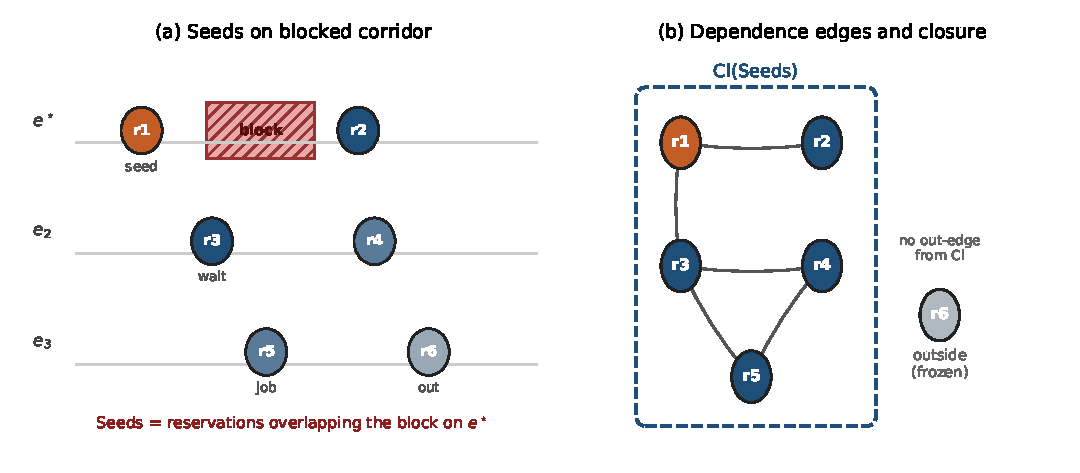
\includegraphics[width=\linewidth]{figures/fig_strc_closure}
\caption{Construction of the reservation impact set.
(a)~The occupancies overlapping the corridor blockage window serve as starting
points;
(b)~taking the transitive closure along the four kinds of dependency edge
(yielding, plus the three successor kinds: same vehicle, same job, same machine)
gives \(\mathrm{Cl}(\mathrm{Seeds})\), while the occupancies outside the set keep
the original plan.}
\Description{Two small schematic panels. (a) On a space--time diagram a blockage
window covers several occupancies, which are marked as starting points. (b)
Taking the transitive closure from the starting points along directed dependency
edges yields the shell of the reservation impact set; occupancies outside the
shell have no incoming edge from inside it and keep the original plan.}
\label{fig:closure}
\end{figure}

The comparison arm that delineates the scope on the operation-precedence graph
maps \(T_{\mathrm{impact}}\) into a set of occupancies allowed to be rewritten:
every occupancy whose task label belongs to that impact region and whose
\(t^e>t_{\mathrm{now}}\).
By Proposition~\ref{prop:miss} this set is empty on Class B.
When the boundary is drawn on the reservation impact set we take
\(U=\mathrm{Cl}(\mathrm{Seeds})\).
In the experimental tables the two are denoted R1 and R2.

\subsection{Containment}
\label{sec:containment}

\begin{prop}[Structural closedness]
\label{prop:struct}
For any \(S\subseteq R\) there is no edge \(u\to v\) in \(G_R^\circ\) with
\(u\in\mathrm{Cl}(S)\) and \(v\in R^{\circ}\setminus\mathrm{Cl}(S)\).
Consequently no unfinished occupancy outside the impact set is reachable from
\(\mathrm{Cl}(S)\) along out-edges.
\end{prop}

\begin{proof}
If such an edge \(u\to v\) existed, then \(u\in\mathrm{Cl}(S)\) would give an
unfinished starting occupancy \(s\) with \(s\to^* u\).
Concatenating \(u\to v\) gives \(s\to^* v\), so by Definition~\ref{def:strc} we
would have \(v\in\mathrm{Cl}(S)\), a contradiction.
\end{proof}

Proposition~\ref{prop:struct} says that ``local'' corresponds to an object that
is closed in the graph-theoretic sense: an occupancy outside the impact set is
not the direct successor of any occupancy inside it.
This does not claim that \(G_R\) has enumerated every coupling possible in the
physical world---the edge set is a modelling choice; once the edge set is fixed,
closedness is a corollary of the definition rather than a heuristic radius.

\begin{remark}[The reservation impact set and a smallest rewritable set]
\label{rem:minimality}
Structural closedness says that the impact set is large enough: no occupancy
inside it has a dependency edge leading outside.
It does not say that the impact set is not too large. There are three reasons.

First, \textbf{a smallest rewritable set depends on the repair procedure used,
whereas the reservation impact set does not}.
To call a set \(U\) smallest, one must state ``under what repair capability
\(U\) suffices to restore feasibility''. The smallest \(U\) when reassignment and
resequencing are permitted is not the same set as the smallest \(U\) when only
rerouting is.
The reservation impact set is uniquely determined by \(G_R\) and independent of
the repair procedure---so by definition it is not tied to any one heuristic, and
by the same token it cannot simultaneously be a smallest set of the kind that
depends on the repair procedure.

Second, \textbf{in the sufficient direction the four kinds of edge remain an
over-approximation; in the necessary direction, the one abutment channel we know
of has now been closed}.
A yield edge is created on ``same corridor, different vehicles, overlapping or
abutting'', that is, whenever the intervals overlap, without judging whether the
later vehicle \emph{really} has no option but to wait for the earlier one---if a
bypass exists there, the later vehicle can simply detour and need not be brought
into the rewritable set at all; likewise a same-vehicle successor edge may bring
in the tail of a chain that the delay never reaches.
Both keep the impact set larger than necessary.
Abutment was once a missing edge in the opposite direction: half-open intervals
that meet end to end are legal, the old rule created no edge, yet if the earlier
one is delayed the later one must yield.
It is now folded into the yield edges; the differential probe leaks
\ProbeLeaks\ on \(\NPairs\) pairs (\ProbeLeakPairs;
Section~\ref{sec:limitations}).
This closes only the one channel we have observed and is not a proof that the
edge set is complete.

Third, \textbf{as measured, the impact set is not small}.
Section~\ref{sec:e6} reports that under corridor blockage the reservation impact
set covers on average about \(90\%\) of the occupancies still unfinished after
\(t_{\mathrm{now}}\); in other words, relative to the trivial upper bound of
``bringing every occupancy unfinished at the decision time into the rewritable
set'', the impact set leaves out less than a tenth.
What bounded repair genuinely saves is \emph{not rewriting occupancies that have
already finished} and \emph{not restarting the search}, not cutting the future
down to a small piece.
The point is made again in Section~\ref{sec:e5} and among the limitations, and
the words ``local'' and ``bounded'' should not be read as ``only a very small
piece is touched''.

``Less than a tenth'' is a ratio of the \emph{sizes} of rewritable sets and is
not the same as a difference of rewrite fractions.
Section~\ref{sec:cheap} implements that trivial upper bound as a separate
comparison (RA) and finds that it is precisely this difference of less than a
tenth that brings the rewrite fraction down from \ResFracAllFuture\ to
\ResFracCheapRtwo\ (per cell \RAStabWTL, \(p=\RAStabP\)), while algorithm runtime
and makespan barely change.

What this paper provides, therefore, is a rewritable set that is uniquely
determined by the structure, reproducible, and \emph{sufficient} to restore
feasibility, together with closedness; approaching a smallest rewritable set is a
different problem and is listed as future work (Section~\ref{sec:future}).
\end{remark}

\begin{prop}[A sufficient condition for the fields outside the set to be unchanged]
\label{prop:outside}
Let the set of occupancies allowed to be rewritten be \(U=\mathrm{Cl}(S)\), and
let the level-1 rerouting run as in Section~\ref{sec:level1}:
(i)~the no-entry window has been written into the routing layer;
(ii)~for every \(r\in R^{\circ}\setminus U\) its original fields
\((e,[t^s,t^e),k)\) are pre-committed to the new reservation table and the
pre-commit succeeds;
(iii)~the router is called only for the transports inside \(U\) to generate new
occupancies;
(iv)~the final schedule passes the conflict-free check.
Then in the recovered reservation table \(R'\) the corridor, interval and vehicle
of every \(r\in R^{\circ}\setminus U\) agree with \(\mathcal{S}^0\).
The quantifier here runs over \emph{occupancies} and not over tasks: one
transport may have part of its occupancies inside \(U\) and part outside, in
which case only the part outside is protected by this proposition.
\end{prop}

\begin{proof}
By (ii), the occupancies outside the set have been written into the new table
with their original intervals before the replay begins, and they do not conflict
with the no-entry window (otherwise the pre-commit would have failed).
Step (iii) submits new occupancies only for the tasks inside \(U\), and neither
deletes nor rewrites the already committed intervals outside it.
Hence for a task label outside the set, \((e,[t^s,t^e),k)\) in the new table
equals the pre-committed value, which is to say it equals the value in
\(\mathcal{S}^0\).
Passing the check only rules out conflicts between the new occupancies and the
existing ones; it does not alter the committed fields.
\end{proof}

Premises (i)--(iv) are execution conditions of the rerouting procedure of
Section~\ref{sec:level1} and can be verified against the algorithm one by one;
they are not model-level assumptions of the A1--A5 kind and are therefore not
folded into the numbered assumption system. The proposition additionally relies
on A1 (the initial schedule is feasible, failing which the original fields
outside the set might conflict with one another and the pre-commit would
necessarily fail), A2 (finished occupancies are not revisited) and A4 (corridor
exclusivity).

\begin{remark}[How premises (ii) and (iii) can each fail]
\label{rem:precommit}
If the pre-commit fails because ``an occupancy outside the set overlaps the
no-entry window'', then \(S\) failed to cover every occupancy overlapping the
blockage window and the starting set is incomplete.
If rerouting fails because of a transport--operation handover and thereby
triggers the scope escalation of Section~\ref{sec:scope_escalation}, then the new
rewritable set satisfies \(U'\supsetneq U\), and
Proposition~\ref{prop:outside} holds only for the occupancies that end up outside
the final rewritable set.
Escalation puts feasibility ahead of rewriting as little as possible, and is
reported separately in the experiments.
There is a further failure mode outside the controllable range of the
proposition, but easy to produce in an implementation: premise (iii) requires the
router to generate new occupancies \emph{only} for the transports inside \(U\).
If the implementation decides whether to reroute at a granularity coarser than
an occupancy (a whole transport, say, or a whole operation), then occupancies
outside \(U\) get rewritten along the way and the conclusion of the proposition
ceases to hold---not because the proposition is wrong but because its premise was
not met. Remark~\ref{rem:e2b_history} records an episode in which our own
implementation rerouted per whole transport.
\end{remark}

\subsection{Structural predictability}
\label{sec:structure}

The size of the reservation impact set is not a tunable parameter but a quantity
uniquely determined by \(G_R\): once the schedule and the network are given, it
has no radius left to tune.
Section~\ref{sec:instscale} scales instances from \(8\times4\times4\) up to
\(\ScaleJobsHi\times\ScaleMachHi\times\ScaleMachHi\), and the share of the impact
set fluctuates between \ScaleCloLo\ and \ScaleCloHi\ without deteriorating with
size (this ratio uses the whole table as denominator, and its attainable upper
bound is about \ScaleAliveShare; with the rewritable set as denominator it is
\ScaleCloAliveLo--\ScaleCloAliveHi).
``Local'' is therefore measurable rather than a radius fixed by hand; but it is
not small, see Remark~\ref{rem:minimality}.

As to \emph{which} structure corresponds to a larger impact set, the experiments
return a negative reading.
We first examine a family of measures computed from the network alone, which do
not vary with the current schedule: the minimum number of corridors that must be
cut to separate the load/unload point from the rest of the shop, that is the
load/unload minimum cut, together with the funnel share; below we call this
family the static cuts.
\textbf{The size of the impact set is not determined by the static cuts.}
On our own layouts of equal size, the relative sizes under different
boundary-blockage protocols either fall within a very narrow band or, where a
direction does appear, have heavily overlapping values across random seeds;
switching to a batch of networks not designed by us, the load/unload minimum cut
and the funnel share \emph{take constant values}, while the share of the impact
set moves substantially when three machine configurations (\(6\), \(7\) and
\(8\) machines) are placed on one and the same network---a constant quantity
cannot explain a varying one (Section~\ref{sec:e4}).
This negative result bears only on the proposition that the static cuts can
explain the size of the impact set, and does not amount to ``structure is
unrelated to the size of the impact set''. The number of public networks
available is limited and the latter question remains undecided.
The next candidate characterization should be a quantity that varies with the
schedule rather than a purely topological one (Section~\ref{sec:future}).

%% =====================================================================
\section{Bounded repair on the reservation impact set}
\label{sec:repair}
%% =====================================================================

Figure~\ref{fig:framework} gives an overview of this section: the set \(U\) of
occupancies allowed to be rewritten is first delineated as the reservation impact
set; the transports inside it are then rerouted while the original plan is kept
outside it; and if feasibility is still not attained, \(U\) is enlarged and the
attempt repeated.
The comparison arm that delineates the scope on the operation-precedence graph
replaces only the provenance of \(U\); the global-rescheduling comparison
searches anew within a time limit.
All methods share one and the same corridor network, time-window router and
conflict-free checker.

\begin{figure}[t]
\centering
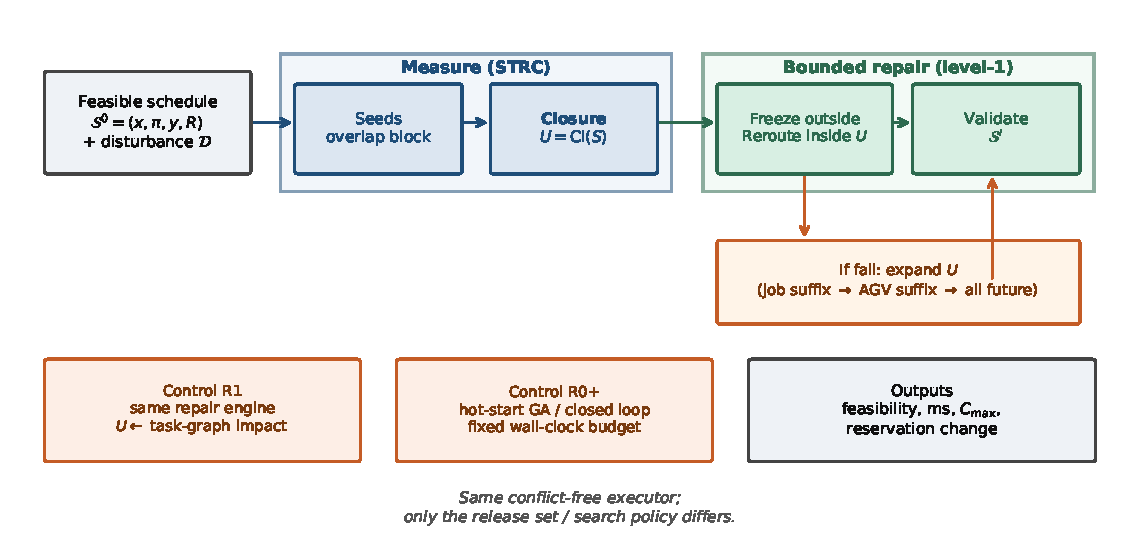
\includegraphics[width=\linewidth]{figures/fig_strc_framework}
\caption{Bounded repair with the boundary drawn on the reservation impact set.
Top row: the impact set is obtained from the starting occupancies and rerouting
follows; middle row: the rewritable scope is enlarged after a failure;
bottom row: the comparison that draws the boundary on the operation-precedence
graph, the warm-started global-rescheduling comparison, and the output measures.
The figure shows only the three method-level paths; three further comparisons
live in the millisecond band (Section~\ref{sec:cheap}).}
\Description{A three-row flow chart. Top row: once the disturbance arrives, the
reservation impact set is obtained from the starting occupancies, the occupancies
inside it may be rewritten while those outside keep the original plan, and the
original vehicle is then rerouted. Middle row: when rerouting fails, the
rewritable set is enlarged in the order job suffix, same-vehicle suffix, all
unfinished occupancies, and the attempt is repeated. Bottom row: two comparisons,
one delineating the scope by the impact region on the operation-precedence graph
and one running a warm-started global search; the three paths feed into one set
of output measures.}
\label{fig:framework}
\end{figure}

\subsection{Rewritable, kept as planned, and level-1 rerouting}
\label{sec:level1}

Given a set \(U\) of occupancies allowed to be rewritten, level-1 rerouting keeps
the original vehicle assignment and machine assignment and replays in the
original sequence.
Rerouting is split by corridor leg: a leg a vehicle has already traversed at
\(t_{\mathrm{now}}\) is history and is pre-committed unchanged, and rerouting
resumes from the node where the vehicle then stood; a granularity coarser than a
leg would rewrite history (Remark~\ref{rem:e2b_history}).
Algorithm~\ref{alg:replay} states this primitive;
Algorithm~\ref{alg:strc_repair} wraps the reservation impact set around it and
enlarges \(U\) on failure.

\begin{algorithm}[t]
\caption{Level-1 rerouting replay \(\textsc{ReplayReroute}\)}
\label{alg:replay}
\begin{algorithmic}[1]
\Require schedule \(\mathcal{S}^0=(x,\pi,y,R)\), disturbance \(\mathcal{D}\), rewritable set \(U\), instant \(t_{\mathrm{now}}\)
\Ensure schedule \(\mathcal{S}'\), or failure
\State write \(\mathcal{D}\) into the routing layer
  \Comment{blockage: no-entry window; slowdown: \(\tau\) on the overlapping part}
\State let \(R'\) be an empty table
\For{every occupancy that may not be rewritten: all those outside the set, and those \(r\in U\) with \(r.t^e\le t_{\mathrm{now}}\)}
  \State pre-commit the original fields \((e,[t^s,t^e),k)\) to \(R'\)
    \Comment{the second kind is the history of A2; omitting it amounts to rewriting history}
  \If{it conflicts with the blockage window}
    \State \Return failure
      \Comment{the starting occupancies did not cover those overlapping the window}
  \EndIf
\EndFor
\For{every \(r\in U\), in the original sequence}
  \State resume from the node of that vehicle at \(t_{\mathrm{now}}\) \Comment{the traversed legs were already committed above and are not submitted twice}
  \State call the time-window router on the current \(R'\) and submit the new occupancies
    \Comment{finished occupancies are not rewritten}
\EndFor
\State advance the idle times of the machines and the ready times of the jobs according to \(\pi\)
\State check independently: conflict freedom, no residue in a no-entry window, the slowdown absorbed on the overlapping part, fields outside the set unchanged
\If{the check passes}
  \State \Return \(\mathcal{S}'=(x,\pi,y,R')\)
\Else
  \State \Return failure
\EndIf
\end{algorithmic}
\end{algorithm}

The breadth-first pass that delineates the boundary (Definition~\ref{def:strc})
accounts for only a small part of the runtime: one call of
\(\textsc{ReplayReroute}\) also invokes a time-window shortest path once for each
of the \(|U|\) transport segments, and the measured runtime is dominated by the
latter (Sections~\ref{sec:e3} and~\ref{sec:cheap}).
This level opens no population search.
The comparison of Section~\ref{sec:e3} holds Algorithm~\ref{alg:replay} fixed and
replaces only whether \(U\) comes from the operation-precedence graph or from the
reservation impact set, so as to attribute the difference in feasibility rate to
the object the boundary is drawn on.

\subsection{Enlarging the rewritable scope after a failure}
\label{sec:scope_escalation}

Enlarging the rewritable scope has precedents of its own. Local
Rescheduling~\cite{kuster2007local} widens a time window step by step until
feasibility is reached; AOR collects downstream operations along job successors
and same-machine successors (Section~\ref{sec:rw_aor}).
We enlarge \(U\) along reservation dependency edges rather than along a time
window.
These steps serve to put the impact set to work: when rerouting fails, the
occupancies that must be rewritten are still enlarged first, rather than a global
search being started at once.
Section~\ref{sec:protocol} explains why the boundary-ablation experiment must
switch this step off.

When keeping the occupancies outside the set is too tight,
Algorithm~\ref{alg:replay} may fail a check such as the transport--operation
handover.
In that case \(U\) is enlarged in the following order and the same rerouting
procedure retried:
(i)~\(U\leftarrow U\cup\{\)the unfinished occupancies of the same-job suffix of
each operation currently in \(U\)\(\}\);
(ii)~\(U\leftarrow U\cup\{\)the unfinished occupancies of the same-vehicle suffix
of the vehicles involved\(\}\);
(iii)~\(U\leftarrow\{\,r\in R:\ r.t^e>t_{\mathrm{now}}\,\}\) (bring every
occupancy unfinished at the decision time into the rewritable set).
After the enlargement it is still a deterministic single-pass rerouting.
Experiments show that this step can pull the feasibility rate up to the whole
sample while keeping the algorithm runtime at the order of milliseconds to a few
tens of milliseconds (Section~\ref{sec:experiments}).
The step also makes the runtime non-monotone in the disturbance fraction
\(\varphi\), because two effects run in opposite directions: at a small fraction
the initial impact set is tight and escalation is needed more often, whereas at a
large fraction the initial \(U\) is already loose and one round often succeeds,
but that single round has more transports to reroute (readings in
Section~\ref{sec:scale}).

\subsection{Comparison with global rescheduling}
\label{sec:vs_r0}

The global-rescheduling comparison searches anew within a time limit, under the
same prohibition constraints and starting from the original schedule (denoted
R0+).
Internally \((x,\pi)\) is encoded as a chromosome; one \emph{decoding} means:
following the assignment and sequence of that chromosome, call the time-window
router of Section~\ref{sec:reservation} for every transport from the beginning on
a reservation table loaded with the no-entry window, obtaining a new \(R\) and a
new \(C_{\max}\).
R0+ repeats the decoding and is allowed to change the chromosome; the RD arm of
Section~\ref{sec:cheap} decodes once and does not change the chromosome.
The decoding of R0+ does not rewrite occupancies that have already finished:
those are pre-committed, and only the operations not yet started are scheduled
from \(t_{\mathrm{now}}\) onwards (Section~\ref{sec:e5}).
The comparison is warm-started rather than searching from scratch, so as not to
discard the assignment and path information already present in the original
schedule.
R0+ may reassign and resequence and is therefore more likely to shorten
\(C_{\max}\), but its algorithm runtime is set by the budget.

Bounded repair is not better than R0+ on makespan.
Section~\ref{sec:e5} shows that R0+ is already ahead at the smallest budget
level, and since R2 is a single fixed point while R0+ is non-increasing in the
budget, adding budget produces no crossover either.
The strength of bounded repair is its algorithm runtime: when the response must be
at the order of milliseconds, it can restore feasibility; when a stoppage of
seconds is permitted, R0+ should be used to shorten \(C_{\max}\).
That the corridor, interval and vehicle of the occupancies outside the set keep
the original plan is guaranteed only under the conditions of
Proposition~\ref{prop:outside}, and is observed partially in the experiments.

Comparing against R0+ alone leaves one question open: within the millisecond
band, is a boundary drawn on the impact set needed at all?
Implementing ``do not restrict the scope by the impact set'' directly answers it,
and we do so in three ways: a global right shift (RS) decides nothing about which
occupancies are affected and merely pushes the unfinished occupancies as a whole
past the end of the blockage; re-decoding of the original chromosome (RD) does not
change the chromosome and runs a single pass of fixed-prefix decoding;
\textbf{RA} brings every occupancy unfinished after \(t_{\mathrm{now}}\) into the
rewritable set and then runs \emph{exactly the same} rerouting procedure as
Section~\ref{sec:level1}, so that it differs from our method in the single item
``which occupancies may be rewritten''---it is the only comparison that isolates
the reservation impact set on its own.
All three are at the order of milliseconds and constitute comparisons for bounded
repair \emph{within the same runtime band}; their definitions and readings appear
in Section~\ref{sec:cheap}.

Algorithm~\ref{alg:strc_repair} puts this section and the previous one together,
matching Figure~\ref{fig:framework}.

\begin{algorithm}[t]
\caption{Bounded repair based on the reservation impact set (level-1 rerouting + scope escalation)}
\label{alg:strc_repair}
\begin{algorithmic}[1]
\Require schedule \(\mathcal{S}^0\), disturbance \(\mathcal{D}\), instant \(t_{\mathrm{now}}\)
\Ensure schedule \(\mathcal{S}'\), or failure
\State \(S \gets \mathrm{Seeds}(\mathcal{D})\);
      \(U \gets \mathrm{Cl}(S)\)
\For{round \(=0,1,2,3\)}
  \State \(\mathcal{S}' \gets \textsc{ReplayReroute}(\mathcal{S}^0,\mathcal{D},U,t_{\mathrm{now}})\)
  \If{\(\mathcal{S}'\) is feasible}
    \State \Return \(\mathcal{S}'\)
  \EndIf
  \State update \(U\) by the escalation rule \Comment{job suffix / same vehicle / all unfinished}
\EndFor
\State \Return failure
\end{algorithmic}
\end{algorithm}

%% =====================================================================
\section{Experiments}
\label{sec:experiments}
%% =====================================================================

\subsection{Protocol}
\label{sec:protocol}

\textbf{Network, router and instances.}
The lower-level network, the time-window router and the independent checker are
fixed. The expanded matrix uses \textbf{five instances}: the small example
\texttt{example\_3x3x2}, the congested example \texttt{congested\_8x4x4}, and
three \texttt{S8x4x4} layouts \texttt{high}, \texttt{funnel} and \texttt{mid}.
The last three have the same size and the same flexibility and differ only in
corridor topology, so differences in the size of the reservation impact set among
them can be attributed to topology rather than to problem size.
The five come from two sources: the first two are hand-written layouts (the small
example for step-by-step checking, the congested one being a dumbbell topology),
while the last three are produced by our instance generator, whose
parameters---jobs \(\times\) machines \(\times\) AGVs, congestion level, \(H\),
\(F\)---are encoded in the instance file name together with the
\textbf{generation seed}; all three were generated with seed \(42\).
\textbf{The generation seed and the run seeds below are two different things}:
the former fixes the instance itself, the latter fix the disturbance injection
and the search process; that both happen to take the value \(42\) is a
coincidence, and nothing is shared.
\textbf{Ten random seeds are used}, namely \(42\), \(7\), \(2024\), \(99\),
\(123\), \(13\), \(1\), \(777\), \(31415\) and \(8\), giving
\(\NInst\times\NSeeds=\NPairs\) instance--seed pairs.
Every per-cell comparison, win/loss count and paired test in this paper is
aligned on the key (instance, seed): under one key all methods read the same
initial solution, the same blockage and the same decision time.
The initial schedule is obtained by replaying the time-window router of
Section~\ref{sec:reservation} in sequence order, and it passes the independent
conflict-free check; under one instance--seed pair all comparison methods share
that initial solution.
This paper does not depend on how \(\mathcal{S}^0\) was found, only on its being
feasible before the disturbance.

\textbf{Implementation and environment.}
Every experiment is implemented in pure standard-library Python with no
third-party numerical package; the lower-level network, the time-window router
and the independent checker reuse the same implementation as the static
integrated work.
Runs are single-machine and single-threaded with no parallelism: Intel Xeon
W-1270 (\(8\) cores, \(16\) threads), \(64\)\,GB of memory, Windows 10,
interpreter CPython \(3.7.6\) (\(64\)-bit).
Since no third-party numerical package is involved, reproduction does not require
pinning dependency versions; \(3.7\) is the interpreter we measured, and higher
versions were not re-run one by one.
All timing readings were obtained under the single-machine, single-threaded
conditions above, and a different machine would shift them all, so every
conclusion about runtime in this paper is stated as a \emph{ratio} or an
\emph{order of magnitude} and never argued from absolute milliseconds.

\textbf{Code and data availability.}
The material needed for reproduction comes in three parts: the upper-level
bounded repair together with the experiment driver, the lower-level network and
time-window router, and the instances, disturbance inputs and all per-cell
readings (CSV).
All three are submitted together with the scripts that regenerate every table and
figure, and are provided during review as an \textbf{anonymous repository} (see
the link attached in the submission system; the repository contains no
author-identifying information); upon acceptance it becomes a public repository
registered with a DOI on a permanent archiving service, and this section will
then be completed with that DOI.
Every table and figure can be traced in the repository to the script and the CSV
that produced it, and the instances listed in Table~\ref{tab:instscale} are
distributed with the repository as well.

\textbf{Second batch: externalizing the provenance of the layouts.}
The layouts of the five instances above were all designed by us, and three of
them, of equal size, further belong to one dumbbell family (they differ only in
the exit of the load/unload point and in the number of parallel lanes in the
middle, that is, in capacity and not in geometry).
So that the layouts are no longer of our choosing, a second batch of \NPubInst\
instances was run: the grid size of the network, the placement of the load/unload
station and of the machines, and the removed edges were transcribed item by item
from the layout figures of Appendix A of Lyu et al.~\cite{lyu2019approach}, and
the transcription was reconciled field by field, by script, against the
machine-readable encoding supplied with the van Os toolset.
The number of machines is therefore fixed by the layout rather than chosen by us,
and ranges from \(4\) to \(8\).
The same ten random seeds are used, giving \NPubPairs\ instance--seed pairs in
total.
The two batches are \emph{matched parameter for parameter}: the number of jobs,
the number of AGVs, the number of operations per job, \(H\), \(F\) and the
calibration target of the transport-to-processing time ratio are all identical,
so the difference between the batches can be attributed cleanly to the provenance
of the layouts.

That appendix gives six layouts in all (\(3\) to \(8\) machines).
The \(3\)-machine one is not used: with \(F=0.6\) fixed, \(|M|=3\) gives an
average of \(1.8<2\) eligible machines, which is incompatible with ``at least two
eligible machines per operation'', and relaxing \(F\) for a single layout would
introduce one more variable.

The remaining five \textbf{live on only \NPubNets\ distinct networks}, which must
be stated first: the \(4\)-machine and \(5\)-machine layouts share one
\(4\times 4\) grid (with the same single edge removed), and the \(6\)-,
\(7\)- and \(8\)-machine layouts share one \(5\times 5\) grid (with the same two
edges removed); the five differ in the number of machines and in \emph{where the
machines sit}, not in network geometry.
This is how the original release itself is organized and not a choice of ours.
Hence when Section~\ref{sec:e4} reads this batch, \textbf{the number of
independent samples along the dimension of network geometry is \NPubNets\ and not
\NPubInst}, whereas along the dimension of machine placement there are
\NPubInst; the statements below follow this division strictly.

Three conventions must be declared up front.
\textbf{First, the per-leg travel times are not original data.} Lyu published
per-leg durations for a single example instance only, and those values are not
uniform; the per-leg durations of the Appendix-A layouts have never been
published. They are therefore filled in here as ``all edges of equal
weight''---structurally consistent with the assumption of a constant single-step
duration in the van Os model, differing only in the scale of the time unit.
\textbf{Consequently the results of this batch must not be compared in any way
with the reference values of Lyu or of van Os}; what it provides is a set of
topologies not designed by us, not a benchmark to be matched.
\textbf{Second, the load/unload points were merged.} The original layouts have
separate loading and unloading stations, whereas we have a single load/unload
point, so the loading station at which the vehicles start plays that role and the
unloading station degenerates into an ordinary grid node.
\textbf{Third, the job data were not borrowed along with the layouts.} In the
public families we have measured, the mean transport duration is only a few per
cent of the mean processing duration, so transport barely produces contention
there; importing the job data as well would degenerate corridor contention, and
with it the whole set of conclusions about it, to the point of being
unobservable. Only the network is externalized.
A further family of layouts shipped with the same toolset (its directory is
labelled Liu 2023) is not included in this batch: the data statement of those
layouts permits diagonal movement, whereas our corridors are 4-adjacent; and
accepting diagonal movement would require changes to the lower-level router
rather than to the instances.

\textbf{Disturbances.}
Unless noted otherwise, \(t_{\mathrm{now}}=0.35\,C_{\max}(\mathcal{S}^0)\).
E1--E3 and E5 impose a single-window blockage on a busy corridor; E6 adds three
further disturbance types at the same \(t_{\mathrm{now}}\); the scale sweep sorts
the future operations by their earliest future reservation and takes the
reservation windows of the leading fraction \(\varphi\) as micro-blockages
(without merging them).

\textbf{Comparison methods.}
R1: the boundary drawn on the impact region of the operation-precedence graph +
level-1 rerouting, with \(\theta=2\) throughout (the value affects only the size
of \(|U_{R1}|\) under Class-A disturbances; by Proposition~\ref{prop:miss} every
finite \(\theta\) yields the empty set on Class B); its delineation rule is taken
from the operation-level local rescheduling described in
Section~\ref{sec:rw_aor} and reimplemented by us.
Item by item, the delineation rule ``take the affected operation set to be the
directly disturbed operations and extend it backwards along the precedence within
a job'' corresponds to
AOR~\cite{abumaizar1997rescheduling,subramaniam2003maor}; whereas
\emph{truncating the extension at \(\theta\) hops} and \emph{mapping the operation
set into the corridor reservations that must be released} are both fixed by us,
since the original settings have no reservation table and this mapping has no
counterpart there; the rerouting and replay components are shared with R2, so
that the two differ only in the object the boundary is drawn on.
R1 is therefore the comparison obtained by ``moving that delineation rule into
the reservation setting of this paper'' and is \textbf{not a reproduction of the
cited work}; its readings in Section~\ref{sec:e3} say only that the delineation
rule returns an empty scope in this setting, and constitute no evaluation of the
original method in its own setting.
R2/\STRC: the boundary drawn on the reservation impact set + level-1 rerouting
(the scale sweep switches scope escalation on; E3 and E5 switch it off).
R0+: global rescheduling that starts from the original schedule and searches anew
within a time limit---a genetic algorithm with population \(40\), the chromosome
of the original schedule placed in the initial population, and decoding using the
same fixed-prefix decoding as RD (occupancies before \(t_{\mathrm{now}}\) may not
be rewritten); \emph{no generation cap and no early-stopping threshold} are set,
the only termination condition being the wall-clock budget, whose values are given
in Section~\ref{sec:e5}.
RS: the global right shift, which draws no boundary on the impact set and does not
reroute (Section~\ref{sec:cheap}).
RD: re-decoding of the original chromosome, that is the cheaper global
recomputation in this implementation (same section).
RA: no restriction of the scope by the impact set, but rerouting retained---every
occupancy unfinished after \(t_{\mathrm{now}}\) is brought into the rewritable
set and everything else is identical to R2, so as to isolate the reservation
impact set on its own (same section).
These five comparisons span the plane ``is a boundary drawn \(\times\) how much is
recomputed'': R1 and R2 differ only in the \emph{object} the boundary is drawn on,
RA and R2 differ only in \emph{whether} a boundary is drawn at all (the rerouting
procedure being identical), RS neither draws a boundary nor reroutes but pushes
everything back, and RD and R0+ recompute globally without drawing a boundary on
the impact set, differing only in how many generations they search.

\textbf{Budget conventions.}
The methods are not compared at a common budget level, and this must be said
first: R1, R2, RS, RD and RA are all one-shot deterministic repairs that stop
when done, their runtime being fixed by instance size and impact-set size rather
than by a budget setting; only R0+ terminates on a wall-clock budget.
There is therefore no alignment in wall clock, generation count or evaluation
count between R0+ and the other methods, and every reading involving R0+ is to be
understood as ``the reading at the given budget''; only the four-method comparison
of Section~\ref{sec:cheap} is a comparison within one budget level (all of them
stop when done).
Wall-clock runtimes are reported per batch and are not read across batches.

\textbf{One convention that must be stated clearly.}
Scope escalation \emph{must be switched off} in E3. Left on, R1 would succeed
incidentally by ``escalating all the way until every unfinished occupancy is in
the rewritable set'', and what would be measured is no longer the difference
between the objects the boundary is drawn on but the fallback capability of the
escalation rule.
Escalation itself works (it pulls the feasibility rate to the full sample in the
scale sweep), but it is orthogonal to the variable under test, and is therefore
switched off throughout the boundary ablation.
That endpoint is not thereby avoided: it is exactly the RA arm of
Section~\ref{sec:cheap}, where its cost is measured cell by cell as an
independent comparison.

\textbf{What each of the two batches is responsible for.}
The two batches are not two samples of the same body of evidence; they answer
different questions, and each section of this chapter is supported by one of them
only.
The main batch answers \emph{whether the phenomenon exists and whether the
mechanism is clean}: under a Class-B disturbance the boundary drawn on the
operation-precedence graph returns an empty scope while the original schedule is
infeasible (Section~\ref{sec:e1}); the reservation impact set contains that scope
and the fields outside the set are invariant (Section~\ref{sec:e2}); and under one
and the same rerouting procedure only the object the boundary is drawn on is
replaced (Section~\ref{sec:e3}).
All three require complete control over the instance parameters, especially the
transport-to-processing time ratio---which decides whether corridor contention
exists at all---and the public families cannot provide such control
(Section~\ref{sec:limitations}, limitation 4).
The second batch answers a different question: \emph{whether these phenomena hold
only on the layouts we chose ourselves}. It is therefore used only for
reproduction and produces no new performance readings
(Section~\ref{sec:pubrepro}).

Two points deserve emphasis. First, \textbf{the second batch is used to test
whether the phenomena hold only on the layouts we chose ourselves}, and to narrow
the conclusion on structural predictability (Section~\ref{sec:e4}).
Second, \textbf{only the single item E4 must be read across both batches}: the
three equal-size layouts of the main batch belong to one family and their
geometric differences are small, so on them the two explanations ``the measure is
too coarse'' and ``the instance set does not differ enough geometrically'' are
confounded; and the external layouts, without a parameter-matched
self-designed control, give no way to judge whether the movement in their
impact-set share is large enough.
The conclusions of the other sections stand on the main batch alone, and the
second batch only strengthens their external validity.

\textbf{Statistical conventions.}
There is exactly one inferential test in this paper: the difference in rewrite
fraction between R2 and RA in Section~\ref{sec:cheap}, using a two-sided Wilcoxon
signed-rank test, paired on the (instance, seed) key described above.
Because this is the only test performed, there is no multiple comparison and no
correction was applied; the per-cell win/loss counts, means and medians elsewhere
are all \emph{descriptive} statistics and no significance is asserted for them.
The accompanying effect size is reported as a Hodges--Lehmann estimate of
\(0.037\), with a \(95\%\) bootstrap confidence interval
\([0.018,\,0.074]\) (percentile method, \(10^4\) resamples, fixed random seed);
the mean of the paired differences is \(\RAStabMean\), interval
\([0.039,\,0.093]\).
Dispersion is reported as an interquartile range: for the rewrite fraction it is
\(0.073\) under R2 and \(0.062\) under RA.
% selfcheck:allow-num 0.073 is the interquartile range of the R2 rewrite fraction; it is numerically equal to \RAStabMeanNet (the mean reduction after the coincident cells are removed) but comes from a different source.
Because \(18\) of the \(50\) cells happen to tie between the two methods, the
lower end of the interval for the \emph{median} paired difference touches
\(0\)---this is recorded as it stands, and it shows that ties make up a third of
the win/loss count.
The tables of the other batches give means, medians and counts only, without
intervals.

\subsection{E1: the operation-precedence graph returns an empty scope}
\label{sec:e1}

This section asks one thing only: what scope each of the two ways of drawing the
boundary returns under a Class-B disturbance, with no comparison of repair
quality.
Table~\ref{tab:e1} and Figure~\ref{fig:e1e3} (left) summarize the expanded
results of Proposition~\ref{prop:miss} under the corridor-blockage protocol of
Section~\ref{sec:protocol}: on \(\PassMiss\) of the samples
\(T_{\mathrm{impact}}=0\), the starting occupancies and the reservation impact set
are non-empty, and the original schedule is infeasible after the blockage.

As the paragraph following Proposition~\ref{prop:miss} warns, the weight in
reading this table should fall on the \emph{second} clause.
Table~\ref{tab:e1} folds three conditions into a single ``C1 pass'' column and
counts them together, but the three are not of the same nature and must be read
apart; the per-cell readings are in the columns \texttt{n\_T\_impact} and
\texttt{feasible\_after\_block} of the data file \texttt{e1\_miss.csv}.
Among them, \(T_{\mathrm{impact}}=0\) is a corollary of the Class-B convention of
Definition~\ref{def:task_impact}: it makes visible that ``the
operation-precedence graph cannot, by definition, reach a corridor blockage'', but
it is not itself a finding.
What is non-trivial is that the latter column is uniformly false---the schedule
\emph{is} already infeasible.
Only the two together constitute the counterexample.

\begin{table}[t]
\centering
\caption{E1, the operation-precedence graph returns an empty scope under corridor
blockage (\(\NSeeds\) random seeds per instance, \(\NPairs\) pairs in total).
\(|R|\) is the number of occupancies in the whole table and \(\mathrm{Cl}/|R|\)
the share of the reservation impact set in it. Means are taken over the seeds.
Dispersion is reported as an interquartile range (IQR): the per-instance IQR of
\(\mathrm{Cl}/|R|\) lies between \EoneFracIqrLo\ and \EoneFracIqrHi, the median
over the \(\NPairs\) pooled pairs is \EoneFracMed, and the spread is
\EoneFracMin--\EoneFracMax; the between-instance and between-seed variation of
this share are thus of the same order, and the mean alone should not be read.
``C1 pass'' counts the cells on which the three conditions of
Proposition~\ref{prop:miss} hold simultaneously (\(T_{\mathrm{impact}}=0\),
non-empty starting occupancies, and the original schedule infeasible after the
blockage). The last three rows have the same size and the same flexibility and
differ only in corridor topology.}
\label{tab:e1}
\small
\begin{tabular}{@{}lcccccc@{}}
\toprule
Instance & Seeds & C1 pass & mean \(|R|\) & mean \(|\mathrm{Seeds}|\)
 & mean \(|\mathrm{Cl}|\) & \(\mathrm{Cl}/|R|\) \\
\midrule
\texttt{example\_3x3x2}   & 10 & \(10/10\) & \(28.6\)  & \(5.6\)  & \(16.9\) & \(0.59\) \\
\texttt{congested\_8x4x4} & 10 & \(10/10\) & \(85.0\)  & \(15.0\) & \(48.4\) & \(0.57\) \\
\texttt{S8x4x4} (high)    & 10 & \(10/10\) & \(150.5\) & \(15.5\) & \(88.3\) & \(0.59\) \\
\texttt{S8x4x4} (funnel)  & 10 & \(10/10\) & \(149.1\) & \(15.5\) & \(85.4\) & \(0.57\) \\
\texttt{S8x4x4} (mid)     & 10 & \(10/10\) & \(147.6\) & \(15.0\) & \(82.8\) & \(0.56\) \\
\midrule
Total & \(\NPairs\) & \(\PassMiss\) & --- & --- & --- & --- \\
\bottomrule
\end{tabular}
\end{table}

The absolute value of \(|\mathrm{Cl}|\) grows with the instance
(\(16.9\), \(48.4\), \(82.8\)--\(88.3\)), a direct consequence of there being more
occupancies in total; \(\mathrm{Cl}/|R|\), by contrast, falls between
\EoneCloLo\ and \EoneCloHi\ on all five instances and \emph{fails} to distinguish
the three \(\texttt{S8x4x4}\) layouts.
This agrees with the conclusion of Section~\ref{sec:e4}: the experiments provide
no structural measure that reliably predicts the size of the impact set.
As far as the contributions are concerned, this section establishes one thing
only: under a Class-B disturbance the boundary drawn on the operation-precedence
graph returns an empty scope while the original schedule is indeed infeasible; the
particular values of \(\mathrm{Cl}/|R|\) carry no claim.

\subsection{E2: containment}
\label{sec:e2}

Structural containment (E2a) holds on \(\PassClosed\) of the samples (leakage
\(=0\)), in agreement with Proposition~\ref{prop:struct}.
The level-1 repair (without escalation) is feasible on \(\NPairs/\NPairs\) of the
samples.
That the corridor, interval and vehicle of every occupancy outside the set are
unchanged entry by entry (E2b, the observational form of
Proposition~\ref{prop:outside}) likewise holds on \(\PassInvar\) of the samples
(Table~\ref{tab:e2}).

\begin{table}[t]
\centering
\caption{E2, containment (\(\NSeeds\) random seeds per instance; the level-1
feasibility column uses no escalation).
E2a is structural closedness (leakage \(=0\)), and E2b is that the corridor,
interval and vehicle of the occupancies outside the set are unchanged
\emph{entry by entry}.}
\label{tab:e2}
\small
\begin{tabular}{@{}lccc@{}}
\toprule
Instance & E2a closed & Level-1 feasible & E2b outside unchanged \\
\midrule
\texttt{example\_3x3x2}   & \(10/10\) & \(10/10\) & \(10/10\) \\
\texttt{congested\_8x4x4} & \(10/10\) & \(10/10\) & \(10/10\) \\
\texttt{S8x4x4} (high)    & \(10/10\) & \(10/10\) & \(10/10\) \\
\texttt{S8x4x4} (funnel)  & \(10/10\) & \(10/10\) & \(10/10\) \\
\texttt{S8x4x4} (mid)     & \(10/10\) & \(10/10\) & \(10/10\) \\
\midrule
Total & \(\PassClosed\) & \(\NPairs/\NPairs\) & \(\PassInvar\) \\
\bottomrule
\end{tabular}
\end{table}

E2a and E2b must be kept apart, and \emph{a full pass does not promote
Proposition~\ref{prop:outside} to a necessary and sufficient condition}.
E2a is a property \emph{of the graph}, guaranteed by
Proposition~\ref{prop:struct}, and a full pass is what ought to happen; were it
not a full pass, the implementation would disagree with the definition.
E2b is a property \emph{after the repair}, and what it tests is whether the four
premises of the proposition hold under our protocol---not that those premises may
be dispensed with.
In particular, premise (ii) requires that every occupancy outside the set be
pre-committed successfully; if one of them overlaps the no-entry window the
pre-commit fails, which indicates that the set of starting occupancies is
incomplete (Remark~\ref{rem:precommit}), and the proposition does not apply.
Our experiments fall on the side where the premises hold, which is not to say
that any setting will fall on that side.
To close this out in terms of the contributions: E1, E2 and the boundary ablation
of Section~\ref{sec:e3} support the layer of \emph{the object standing up}---the
reservation impact set is uniquely determined by the edge set, closed outwards,
and sufficient to restore feasibility under one and the same rerouting procedure;
how much benefit drawing the boundary on this object buys over not drawing it is
\emph{another layer}, supported only by the RA comparison of
Section~\ref{sec:cheap}.

\begin{remark}[An episode in which an implementation defect was read as a defect of the edge set]
\label{rem:e2b_history}
This column stood at only \(24/\NPairs\) in an earlier batch. The reading at the
time was that ``the dependency edge set fails to cover certain weak couplings'',
and refining the edge set was accordingly listed as the first item of future work.
On review that reading was wrong.
What may be rewritten is a set of \emph{occupancies}, whereas at replay time the
decision to reroute was taken per \emph{operation}---as soon as either the empty
or the loaded segment of an operation fell inside the impact set, the whole
transport was replanned.
So when only the loaded segment entered the impact set, the empty segment of the
same operation was rewritten as well, even though its task label was not in the
rewritable set, and this was recorded as drift outside the set.
The \(84\) drifting occupancies on the \(26\) failing cells were without
exception empty segments of this kind, and \(71\) of them (\(85\%\)) had already
been executed before \(t_{\mathrm{now}}\)---rewriting such a segment also violates
``do not rewrite occupancies that have already finished''.
After the decision was moved to a per-\emph{segment} basis (an empty segment
already executed or not brought into the rewritable set keeps the original plan,
and only the segments genuinely inside the rewritable set are rerouted), the
drift fell to zero.
In other words, what had been measured was not the coverage of physical couplings
by the edge set but the fact that premise (iii) of
Proposition~\ref{prop:outside}, ``call the router only for the transports inside
\(U\)'', had not really been met in the implementation. We record this because it
exemplifies an easy misjudgement: reading a granularity mismatch between
implementation and definition as an insufficiency of the model with respect to the
world.

\textbf{One more layer of the same mismatch remains, and E2b cannot detect it.}
Even after the decision is taken per segment, a transport segment that
\emph{straddles} \(t_{\mathrm{now}}\) is still replanned in its entirety: as soon
as the end time of one of its corridor legs falls after \(t_{\mathrm{now}}\), the
task label of the whole segment enters the rewritable set, and so the legs it had
\emph{already traversed} before \(t_{\mathrm{now}}\) are rescheduled too---which
amounts to sending the vehicle back to the start of the segment to travel it
again, in violation of ``do not rewrite occupancies that have already finished''.
E2b cannot detect this, because the task labels of those legs are \emph{inside}
the impact set and hence outside the comparison range of the fields outside the
set.
It took an independent audit of ``finished occupancies may not be rewritten''
(comparing entry by entry the occupancies with
\(t_{\mathrm{end}}\le t_{\mathrm{now}}\)) to measure it: \(36\) of the \(\NPairs\)
cells contained rewrites of this kind, \(86\) occupancies in all.
After the granularity was refined by one more level---splitting by
\emph{corridor leg}, keeping the traversed legs unchanged, and resuming the
rerouting from the node at which the vehicle actually stood at
\(t_{\mathrm{now}}\)---that audit fell to zero on all \(\NPairs\) cells, with
every pass rate unchanged, \(C_{\max}\) improving on \(6\) cells and worsening on
none.
The readings reported in this paper are the corrected ones. The historical
readings in this remark (\(24/\NPairs\); \(84\) occupancies on \(26\) cells;
\(86\) occupancies on \(36\) cells) come from the batches before the correction
and from one independent audit of ``finished occupancies may not be rewritten'';
they appear in none of the tables of this paper and support no claim.
\end{remark}

\subsection{E3: boundary ablation}
\label{sec:e3}

Table~\ref{tab:e3} and Figure~\ref{fig:e1e3} (right) hold the level-1 rerouting
fixed and \emph{switch off} scope escalation.
On Class B, the rewritable set of R1 is empty and infeasible on
\(\NPairs/\NPairs\) of the samples, while R2 is feasible throughout.

This is the strongest comparison in the paper, but its force comes from
\emph{differing in one item only} and not from the size of the numbers: the same
rerouting procedure, the same initial solution, the same \(t_{\mathrm{now}}\), the
same random seeds and the same blockage window, with \textbf{the sole difference
being which occupancies may be rewritten}.
The contrast \(\FeasRone\) against \(\FeasRtwo\) therefore cannot be attributed to
the quality of a rerouting heuristic---on the R1 side no rerouting is triggered at
all, its rewritable set being empty, and level-1 rerouting is the identity on the
empty set, so the original schedule stays untouched on the blocked corridor.
Put differently, R1 fails not by ``repairing badly'' but by ``judging that no
repair is needed''.
The per-cell runtime of level-1 rerouting has median \(\MsRepairMed\)\,ms and
maximum \(\MsRepairMax\)\,ms; the last column of Table~\ref{tab:e3} is the mean
over the \(\NSeeds\) seeds within each instance, a different convention, and the
two must not be read against each other.
As far as the contributions are concerned, this section pins the cause of the gap
on the object the boundary is drawn on: replacing only that object under one and
the same rerouting procedure moves the rate at which feasibility is restored from
\(\FeasRone\) to \(\FeasRtwo\); this still belongs to the layer of \emph{the
object standing up} and says nothing about the net benefit of the boundary.

Whether the contrast above depends on the calibration of the edge weights is
tested separately. Our corridor weights are uniform, so E1 and E3 were re-run on
the same \(\NPairs\) pairs under three non-uniform weight settings
(\texttt{lognormal}, \texttt{lu\_far}, \texttt{split}; data in
\texttt{weight\_sweep.csv}): the readings for C1 pass and for the empty
operation-precedence scope are unchanged at every setting, R1 remains infeasible on
every cell, and the number of cells on which level-1 R2 is feasible is
\WeightLogRtwo, \WeightLuRtwo\ and \WeightSplitRtwo\ respectively, the single
infeasible cell occurring in the \texttt{split} setting
(\texttt{S8x4x4\_high}, seed \(1\)).
The contrast therefore does not depend on the uniform calibration; but a sweep over
self-assigned edge weights still cannot replace an instance family that publishes
both the network and the per-leg durations (Section~\ref{sec:limitations},
limitation \(4\)).

\begin{table}[t]
\centering
\caption{E3, boundary ablation (no escalation; \(\NInst\) instances \(\times\)
\(\NSeeds\) random seeds).
miss\_B means that on that cell the rewritable set of R1 is empty while that of R2
is not.
The last column is the mean over the \(\NSeeds\) seeds within each instance, a
different convention from the per-cell median in the body.}
\label{tab:e3}
\small
\begin{tabular}{@{}lccccc@{}}
\toprule
Instance & miss\_B & R1 feasible & R2 feasible & mean \(|U_{R2}|\) & R2 runtime/ms \\
\midrule
\texttt{example\_3x3x2}   & \(10/10\) & \(0/10\) & \(10/10\) & \(16.9\) & \(0.66\) \\
\texttt{congested\_8x4x4} & \(10/10\) & \(0/10\) & \(10/10\) & \(48.4\) & \(2.84\) \\
\texttt{S8x4x4} (high)    & \(10/10\) & \(0/10\) & \(10/10\) & \(88.3\) & \(3.40\) \\
\texttt{S8x4x4} (funnel)  & \(10/10\) & \(0/10\) & \(10/10\) & \(85.4\) & \(5.09\) \\
\texttt{S8x4x4} (mid)     & \(10/10\) & \(0/10\) & \(10/10\) & \(82.8\) & \(3.96\) \\
\midrule
Total & \(\NPairs/\NPairs\) & \(\FeasRone\) & \(\FeasRtwo\) & --- & --- \\
\bottomrule
\end{tabular}
\end{table}

\begin{figure}[t]
\centering
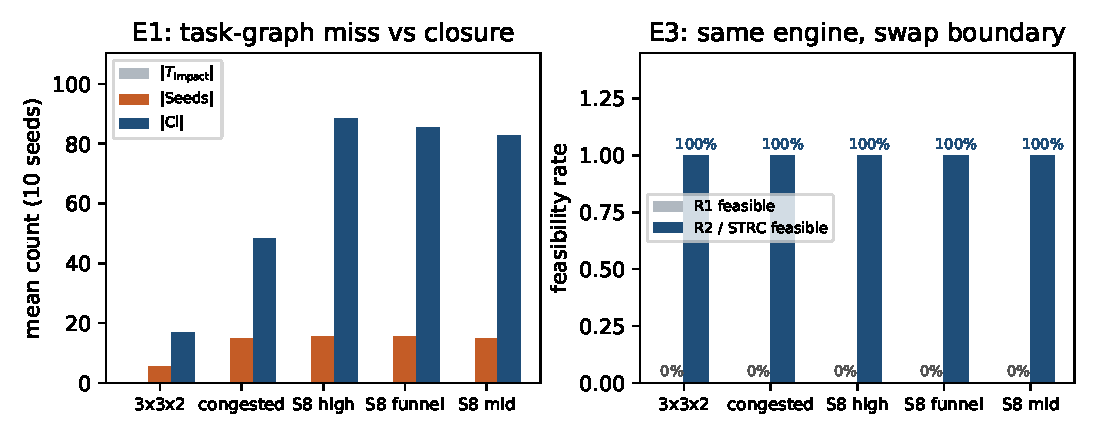
\includegraphics[width=\linewidth]{figures/fig_strc_e1e3}
\caption{Visualization of the expanded E1/E3 results (\(\NInst\) instances
\(\times\) \(\NSeeds\) random seeds, means).
Left: the impact region on the operation-precedence graph is empty while the
starting occupancies and the reservation impact set are not; bar heights are the
means over the \(\NSeeds\) cells of each instance, and the dispersion as an
interquartile range is given in Table~\ref{tab:e1} (the per-instance IQR of
\(|\mathrm{Cl}|\) lies between \(2\) and \(8\); the impact-region series is
identically zero and has no dispersion).
Right: with the same rerouting and only the object the boundary is drawn on
replaced, the feasibility rate of R1 is \(0\) and that of R2 is \(100\%\); this
panel is a per-cell count (\(\NPairs\) cells each), not a mean, and therefore
carries no dispersion.}
\Description{Two bar charts side by side. The left panel gives, for the five
instances, three series of bars: the impact region on the operation-precedence
graph, the number of starting occupancies, and the size of the reservation impact
set; the impact-region series is identically zero while the other two rise with
instance size. The right panel gives the recovery feasibility rates of the two
ways of drawing the boundary: zero on the operation-precedence side and one
hundred per cent on the reservation impact set side.}
\label{fig:e1e3}
\end{figure}

%% Do not put \(\times\) in a section title: it goes into the PDF bookmarks, and
%% hyperref cannot handle math mode there.
\subsection{E6: crossing disturbance types with boundary definitions}
\label{sec:e6}

E1--E3 used corridor blockage as the only disturbance. This subsection opens up
the dimension of disturbance type, adding corridor slowdown, vehicle breakdown and
robotic-arm breakdown on the same \(\NPairs\) pairs, and gives
Table~\ref{tab:e6}.

\textbf{What is measured, first.} On the boundary side, all four types are
reported: how large the impact region on the operation-precedence graph is, how
large the reservation impact set is, and whether the latter contains the former.
On the repair side, all four types are opened up.
Class B still reroutes only: a blockage writes a no-entry window into the
reservation table, while a slowdown reduces progress inside the window by a factor
\(\tau_{\mathrm{mult}}=2\) and keeps the original \(\tau\) outside it, the corridor
remaining passable.
Class A additionally swaps vehicles or reassigns machines, without changing the
sequence; whether the rewritable scope is enlarged does not change the action set
for them.

\begin{table}[t]
\centering
\caption{E6, disturbance type \(\times\) the object the boundary is drawn on
(\(\NPairs\) pairs per type, \(200\) measurements in all; two of the types are
Class B and yield the same starting set by construction, so the number of
\emph{independent} boundary measurements is \(150\), see point three in the body).
\(|R^{\circ}|\) is the number of occupancies unfinished after
\(t_{\mathrm{now}}\).
``R1 empty'' counts the cells on which the boundary drawn on the
operation-precedence graph declares that the disturbance needs no rescheduling.
The last column uses no escalation: level-1 rerouting for Class B, vehicle swap or
reassignment for Class A.}
\label{tab:e6}
\small
\begin{tabular}{@{}llccccc@{}}
\toprule
Disturbance & Class & R1 empty & mean \(|U_{R1}|\) & mean \(|\mathrm{Cl}|\)
 & \(\mathrm{Cl}/|R^{\circ}|\) & R2 feasible \\
\midrule
Corridor blockage      & B & \(50/50\) & \(0.0\)  & \(64.4\) & \(0.92\) & \FeasESixBlock \\
Corridor slowdown      & B & \(50/50\) & \(0.0\)  & \(64.4\) & \(0.92\) & \FeasSlow \\
Vehicle breakdown      & A & \(0/50\)  & \(31.1\) & \(60.6\) & \(0.85\) & \FeasESixAgv \\
Robotic-arm breakdown  & A & \(0/50\)  & \(42.8\) & \(65.9\) & \(0.94\) & \FeasESixRa \\
\bottomrule
\end{tabular}
\end{table}

Four readings. First, \textbf{the A/B dichotomy holds without exception on the
\(150\) \emph{independent} boundary measurements} (the two Class-B disturbances
share one starting set by construction, see point three below, so they are not
counted as \(200\)): both Class-B types return an empty scope on the
operation-precedence graph, and both Class-A types return a non-empty one.
Second, \textbf{\(U_{R1}\subseteq\mathrm{Cl}\) on all \(100\) Class-A
measurements}---so moving to a boundary drawn on the reservation impact set
\emph{loses} none of the occupancies that the operation-precedence graph already
included.
The containment is strict on \(\StrictlyLarger\) of the cells, while on the
remaining \(13\) the two are exactly equal (there the impact set does not leave,
along dependency edges, the set induced by the impact region on the
operation-precedence graph), which is \emph{not} a containment failure.
Among these, the containment on the \(50\) robotic-arm-breakdown cells holds
\emph{by construction}: the starting rule of Definition~\ref{def:seeds}(c) takes
the whole suffix along the job chain, whereas \(U_{R1}\) truncates at
\(\theta=2\) (Section~\ref{sec:protocol}), so what that row verifies is agreement
between implementation and definition rather than an independent finding; the
containment on the \(50\) vehicle-breakdown cells is not given by construction and
is a measured result.
The price is that the rewritable set becomes larger on average: \(31.1\to 60.6\)
for vehicle breakdown and \(42.8\to 65.9\) for robotic-arm breakdown.
Together with the first reading, the reservation impact set is a uniform
strengthening in \emph{coverage} over the operation-precedence boundary on these
four disturbance types---no occupancy already included is lost; it does cost
something in the size of the set, so the two are not a trade-off in coverage.
Third, \textbf{the two boundary rows for slowdown and blockage are identical cell
by cell}, with the same impact-set size on all \(50\) pairs.
This is not two independent validations of the boundary: for both, the starting
rule is ``the unfinished occupancies overlapping the invalidated window'', so by
construction they yield the same starting set and hence the same reservation impact
set. What that row does confirm is that the boundary drawn on the
operation-precedence graph is likewise empty for a slowdown.
Fourth, \textbf{the repair side is full on all four types}, with the per-type
readings in the last column of Table~\ref{tab:e6}, slowdown and blockage sharing
one convention.
The slowdown once multiplied any traversal intersecting the window by \(2\) over
its whole length, and \(13\) cells died on ``the occupancy is too short''---when
there was no free slot for \(2\tau\) inside the window, the entry time was pulled
back into the window while the occupancy was still committed with the original
\(\tau\); \(12\) of them could not pass even with every unfinished occupancy
brought into the rewritable set, so it was not keeping the plan outside the set
that stranded the slowed vehicle.
After the change to scaling only the overlapping progress, level 1 passes fully
and escalation is no longer triggered.
The corridor remains passable, so the physical difference from ``seal the whole
segment and detour'' is still there; it is merely no longer amplified by a factor
applied to the whole segment.
Vehicle breakdown is handled by a vehicle swap, robotic-arm breakdown by
reassignment.
Vehicle swap and reassignment are the actions that implement Class-A recovery, and
serve to complete the repair side of the coverage matrix.

\textbf{This table also gives the measured size of the impact set}
(Remark~\ref{rem:minimality}).
Under corridor blockage the reservation impact set covers about
\(\ClosureAliveFrac\) of the occupancies unfinished after \(t_{\mathrm{now}}\);
relative to the trivial upper bound of ``bring every unfinished occupancy into the
rewritable set'' it leaves out less than a tenth.
What bounded repair genuinely saves is not rewriting occupancies that have already
finished, and not restarting the search---not cutting the future down to a small
piece.
The \(\mathrm{Cl}/|R|\) of Section~\ref{sec:e1}, computed over the whole table and
falling in \EoneCloLo--\EoneCloHi, does not contradict this: the whole table
includes the half already executed before \(t_{\mathrm{now}}\), which was never
modifiable in the first place.
Both conventions are given.
As far as the contributions are concerned, this section extends only
\emph{coverage}---carrying the A/B dichotomy and the containment from one
disturbance type to four; it strengthens no claim and introduces no new object for
the boundary to be drawn on.

\subsection{A case Gantt chart}
\label{sec:case}

\begin{sloppypar}
E1--E3 give counts and feasibility rates across random seeds. To place ``beyond the
reach of the operation-precedence graph, repairable via the reservation impact
set'' on the time axis, Figure~\ref{fig:case} takes one corridor blockage on
\texttt{example\_3x3x2} with seed \(42\), under the same protocol as E2/E3: the
decision time is \(0.35\,C_{\max}\), a single-window blockage on a busy corridor,
level-1 rerouting and no escalation.
\end{sloppypar}

On this instance \(T_{\mathrm{impact}}=\varnothing\), while
\(|\mathrm{Seeds}|=6\) and \(|\mathrm{Cl}|=18\).
Figure~\ref{fig:case}(a) is the machine Gantt chart of the original schedule before
the disturbance: the transport occupancies of the blue operations fall inside the
impact set (and will be rerouted), the grey operations lie outside it
(pre-committed, keeping the original plan); the red dashed line is
\(t_{\mathrm{now}}\) and the light red band is the blockage window.
Figure~\ref{fig:case}(b) is the state after the repair: the time axis of the
operations inside the impact set is rearranged, the schedule regains feasibility
under the blockage, \(C_{\max}:57\to 86\), with a sub-millisecond runtime.
The figure only shows what kind of local modification the statistical conclusions
correspond to, and is not used to compare makespans; the trade-off in makespan
against global rescheduling appears in E5 and the scale sweep below.

\begin{figure}[t]
\centering
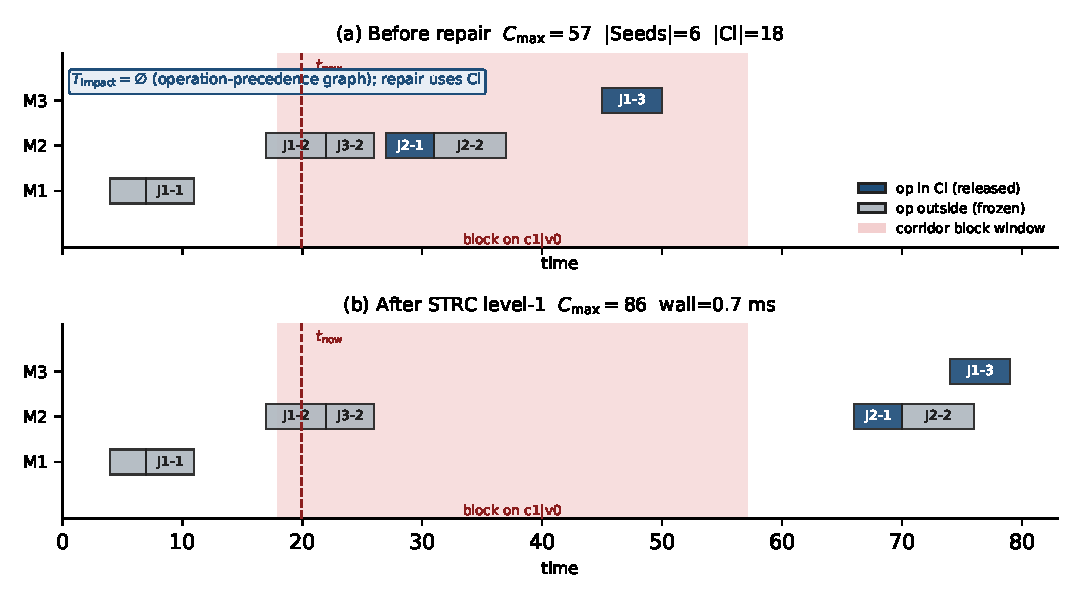
\includegraphics[width=\linewidth]{figures/fig_strc_case}
\caption{Case Gantt chart (\texttt{example\_3x3x2}, seed \(42\)).
(a)~The original schedule before the blockage, coloured by membership in
\(\mathrm{Cl}\);
(b)~after the level-1 repair. The impact region on the operation-precedence graph
is empty; the blue operations are those whose transports inside the impact set are
rerouted.
The figure is an \emph{existence} demonstration: it shows what kind of local
modification the statistical conclusions correspond to, and the change in
\(C_{\max}\) is not taken as a performance reading.}
\Description{Two machine Gantt charts, one above the other. (a) The original
schedule before the blockage, with bars coloured blue or grey according to whether
their transport occupancies fall inside the reservation impact set; a vertical red
dashed line marks the decision time and a light red vertical band marks the
blockage window. (b) The schedule after the repair, in which the time axis of the
blue bars has been rearranged, the grey bars have not moved, and the makespan has
grown from 57 to 86.}
\label{fig:case}
\end{figure}

\subsection{E4: structure (exploratory)}
\label{sec:e4}

Under a blockage of an LU cut edge, the impact-set shares of funnel and high
fluctuate across random seeds (Table~\ref{tab:e4}).
In direction funnel is indeed higher---median \(0.254\) against \(0.204\), mean
\(0.244\) against \(0.229\)---but \emph{the two sets of values overlap heavily}:
funnel falls in \([0.180,0.309]\) and high in \([0.156,0.372]\), the latter
interval containing the former entirely, and a single random seed can reverse the
order (in the \(2024\) column high's \(0.372\) is higher than funnel's
\(0.296\)).
With five random seeds and two layouts, this difference cannot support any
conclusion.
The \(\mathrm{Cl}/|R|\) obtained in Section~\ref{sec:e1} on three equal-size
layouts under the busy-corridor blockage protocol likewise falls in the narrow
band \EoneCloLo--\EoneCloHi\ and equally fails to distinguish the layouts.

\textbf{Only with a batch of layouts not designed by us can the cause of this
negative result be separated.}
The three equal-size layouts belong to one dumbbell family and differ little in
geometry (see Table~\ref{tab:e4pub}: \(9\)--\(11\) nodes, \(8\)--\(12\) corridors,
and an LU cut of only \(1\) or \(2\)); on them ``the measure is too coarse'' and
``the instance set does not differ enough geometrically'' are confounded and cannot
be told apart. The second batch of Section~\ref{sec:protocol} separates the two
(Table~\ref{tab:e4pub}).

\textbf{The direction of the result is the opposite of what was expected, and that
is precisely the point.}
As declared in Section~\ref{sec:protocol}, this batch has only \NPubNets\
independent samples along network geometry, so it \emph{cannot} be used to argue
that ``the impact-set share varies with network geometry''; what it can argue is
something else.
On \emph{one and the same} \(4\times 4\) network, changing only the number and the
placement of the machines from \(4\) to \(5\) moves the median impact-set share
from \PubCloHi\ down to \PubCloLo, a spread of \PubCloSpread; on one and the same
\(5\times 5\) network, three machine configurations (\(6\), \(7\) and \(8\)
machines) give a spread of \PubCloSpreadBig.
For comparison, the three \emph{parameter-matched} self-designed layouts---which
are three \emph{different} networks---fall only in \SelfCloLo--\SelfCloHi, a spread
of \SelfCloSpread.
That is: \textbf{with the network fixed and the machine configuration varying, the
impact-set share can move further than it does across three different networks}---
about fourfold on the \(4\times 4\) network and about one and a half times on the
\(5\times 5\) one. Two qualifications are needed on the numbers of factors varied
on each side: the left-hand side changes the number and the placement of machines
at once, whereas the three self-designed layouts on the right are all
\(4\)-machine and change only the network. It must further be said that the
right-hand baseline is weak: as noted at the start of this section, the three
self-designed layouts differ little in geometry to begin with, so
\SelfCloSpread\ is a \emph{lower bound} on the magnitude of ``changing the
network'', not a representative value.
Taken together, this inequality supports only ``the machine-configuration
dimension cannot be ignored'' and does \emph{not} support ``the effect of machine
configuration exceeds that of network geometry''. What holds on both networks is
the direction of the inequality; the multiples themselves rest on two samples and
should not be read closely.

\textbf{Hence a minimum cut determined by the network alone does not explain the
size of the impact set.}
On these \NPubInst\ external instances, \textbf{the load/unload minimum cut (the
LU cut) is constantly \(2\) and the funnel share constantly \(0\)}---both networks
place the load/unload station at a grid corner, and a corner of a 4-adjacent grid
has exactly two outgoing edges, so this cut is pinned down; the family shipped
with the same toolset (excluded from this batch because it permits diagonal
movement) places the station at the midpoint of a grid edge, with three outgoing
edges.
\textbf{That is, on real layouts this measure takes only a handful of values, all
fixed by the grid position of the load/unload station}, and does not vary
continuously with geometry.
What matters is that \textbf{these two measures do not move at all across the whole
variation described above}, while the quantity to be explained has already moved
by \PubCloSpread.
A quantity with a constant value cannot explain one that varies this much, so it is
not even a matter of ``weak correlation'' but of \emph{having nothing to say}; a
third measure (corridors per node) takes only two values over the whole batch
(\(23/16\) and \(38/25\)) and is likewise insufficient to explain the
within-group variation.

The reading can accordingly be tightened to: \textbf{on these \NPubInst\ external
instances and three self-designed layouts, the static cuts do not explain the size
of the impact set}. This family of measures was designed around the tunable
load/unload throat of the dumbbell layout, and once carried over to real layouts it
degenerates into a constant with no explanatory power.
The alternative direction therefore points at the demand side: what determines the
size of the impact set is not how many paths the network \emph{can} provide but
\emph{where the demand falls}; concrete candidate quantities are given in
Section~\ref{sec:future}.
As far as the contributions are concerned, this section is an \emph{exploratory}
negative result and supports none of them---it says only that the family of static
measures we designed around the dumbbell layout should not be extrapolated, and it
offers no predictive measure in their place.

\begin{table}[t]
\centering
\caption{E4, the impact-set share \(\mathrm{Cl}/|R|\) (blockage of an LU cut edge;
random seeds \(42,7,2024,99,123\)).
The instances of this table have \(12\) jobs / \(8\) machines / \(12\) vehicles and
a transport-to-processing time ratio calibrated to \(4.0\).
\textbf{This convention differs from that of Table~\ref{tab:e4pub}} (which uses
\(8\) jobs / \(4\) machines / \(4\) vehicles, a ratio of \(1.0\), and ten random
seeds); although the two tables share the layout names \texttt{funnel} and
\texttt{high}, \emph{the values must not be compared across tables}; only within
Table~\ref{tab:e4pub} is the comparison like for like.}
\label{tab:e4}
\small
\begin{tabular}{@{}lcccccc@{}}
\toprule
Layout & \(42\) & \(7\) & \(2024\) & \(99\) & \(123\) & Median \\
\midrule
funnel & \(0.254\) & \(0.181\) & \(0.296\) & \(0.309\) & \(0.180\) & \(0.254\) \\
high & \(0.156\) & \(0.204\) & \(0.372\) & \(0.229\) & \(0.184\) & \(0.204\) \\
\bottomrule
\end{tabular}
\end{table}

\begin{table}[t]
\centering
\caption{E4, comparison with the provenance of the layouts externalized (blockage
of an LU cut edge, ten random seeds; \(\mathrm{Cl}/|R|\) as a median).
The whole table is matched parameter for parameter and differs only in the network
and the machine configuration. \textbf{The external instances live on only
\NPubNets\ networks} (\(\mathrm{N}_1\): \(4\times 4\) with one edge removed;
\(\mathrm{N}_2\): \(5\times 5\) with two edges removed), and the rows within a
group \emph{share one network}, differing only in the number and the placement of
the machines; the ``spread'' column is given \emph{within a group}, and since group
\(\mathrm{N}_1\) has only \(2\) rows and the self-designed group \(3\), ratios of
spreads between groups are only an order-of-magnitude reference.
The LU minimum cut and the funnel share \emph{take constant values} throughout the
external batch.
The edge weights are the uniform values supplied by this paper, so this table is
not compared against reference values from the external literature.}
\label{tab:e4pub}
\small
\begin{tabular}{@{}llcccccc@{}}
\toprule
Source/network & Instance & Machines & Nodes/corridors & LU cut & Funnel share & \(\mathrm{Cl}/|R|\)
 & Within-group spread \\
\midrule
External \(\mathrm{N}_1\) & \texttt{LyuL2} & \(4\) & \(16/23\) & \(2\) & \(0\) & \(0.512\) & \\
External \(\mathrm{N}_1\) & \texttt{LyuL3} & \(5\) & \(16/23\) & \(2\) & \(0\) & \(0.305\)
  & \(\PubCloSpread\) \\
\cmidrule{1-8}
External \(\mathrm{N}_2\) & \texttt{LyuL4} & \(6\) & \(25/38\) & \(2\) & \(0\) & \(0.385\) & \\
External \(\mathrm{N}_2\) & \texttt{LyuL5} & \(7\) & \(25/38\) & \(2\) & \(0\) & \(0.422\) & \\
External \(\mathrm{N}_2\) & \texttt{LyuL6} & \(8\) & \(25/38\) & \(2\) & \(0\) & \(0.460\)
  & \(\PubCloSpreadBig\) \\
\midrule
Self-designed & \texttt{high} & \(4\) & \(10/10\) & \(2\) & \(0.286\) & \(0.497\) & \\
Self-designed & \texttt{funnel} & \(4\) & \(9/8\) & \(1\) & \(0.286\) & \(0.491\) & \\
Self-designed & \texttt{mid} & \(4\) & \(11/12\) & \(2\) & \(0.286\) & \(0.446\)
  & \(\SelfCloSpread\) \\
\bottomrule
\end{tabular}
\end{table}

\subsection{E5: the trade-off against global rescheduling}
\label{sec:e5}

This subsection originally set out to find a \emph{crossover point}: bounded repair
ahead when the budget is tight, and warm-started global rescheduling overtaking it
on \(C_{\max}\) once the budget is relaxed.
\textbf{No such crossover exists within the \(0.2\)--\(2\)\,s range measured, and
the absence extrapolates to larger budgets}, the reason being not an insufficient
sample but the shape of the two curves: R2 is a one-shot fixed point, the three
budget levels within a cell sharing one and the same computation, so its
\(C_{\max}\) does not vary with the budget; R0+ reports the best over generations,
and once the random seed is fixed a larger budget merely lets the same search
trajectory run a few more generations, so its \(C_{\max}\) can only decrease.
Once the order of the two is settled at the \emph{smallest} budget level, adding
budget cannot reverse it, so only the smallest level needs to be examined: on the
\(\EfiveCells\) instance--seed cells, R0+ is already strictly better on
\(\EfiveWinMin\) cells, ties on \(\EfiveTieMin\), and is worse on none.

The \emph{direction} of this non-existence must be made explicit: the monotonicity
above extrapolates only to \emph{larger} budgets, and smaller budgets were not
swept.
The same monotonicity indicates that the order should reverse on the low-budget
side---R0+ pays at least one decoding per candidate evaluated
(\(\MsRedecode\)\,ms in the same batch, Section~\ref{sec:cheap}), so given its
population size the wall clock needed merely to evaluate the initial population is
already of the same order as the smallest budget level, whereas R2 needs only
\(\MsCheapRtwo\)\,ms in the same batch and is feasible on every cell.
As the budget is tightened further, then, R0+ will fail to deliver even one
generation, and we make no assertion about the order on that side; the smallest
level measured sits right at this boundary.
This does not affect the direction of our argument---what we are ruling out is
``bounded repair is better on \(C_{\max}\)'', and a reversal on the low-budget side
would favour bounded repair, so we do not take that reading here.

Table~\ref{tab:e5} and Figure~\ref{fig:e5} give the self-designed-layout half:
two instances \(\times\) random seeds \(\{42,7,2024\}\) \(\times\) budgets
\(\{0.2,1,2\}\)\,s.
Section~\ref{sec:pubrepro} re-runs the same protocol on two \emph{external}
layouts with the same code and the same parameters; read together, the two batches
cover \(\EfiveInst\) instances, \(\EfiveCells\) instance--seed cells and
\(\EfivePts\) budget points, with an R0+ win/tie/loss of \(\EfiveWLT\) point by
point, and the monotonicity and the fixed point above were checked cell by cell on
all \(\EfiveCells\) cells.
The limits still have to be stated: \(\EfivePts\) points are \emph{not}
\(\EfivePts\) independent pieces of evidence, since the instance dimension has only
\(\EfiveInst\) members, and this section therefore asserts no significance.
The non-existence within and above the range measured follows from the monotonicity
above and is independent of the sample size; generality along the instance
dimension, however, extends only to these \(\EfiveCells\) cells---whether another
batch of instances would still show no crossover is not tested here.

\begin{table}[t]
\centering
\caption{E5, against warm-started global rescheduling that does not rewrite
finished occupancies (means over \(3\) random seeds).
The ``rewrite fraction'' is the share of rewritten occupancies in the whole table.
This table contains self-designed layouts only, \(2\) instances \(\times\) \(3\)
random seeds \(\times\) \(3\) budget points, i.e.\ \(6\) independent cells;
comparing the two \(C_{\max}\) columns, R0+ is better at every budget point.
Read together with the external-layout batch (Section~\ref{sec:pubrepro}) this
becomes \(\EfiveCells\) cells and \(\EfivePts\) points, with a point-by-point
win/tie/loss of \(\EfiveWLT\).
R2 does not vary with the budget, so the three rows of each instance share one R2
fixed point.}
\label{tab:e5}
\small
\begin{tabular}{@{}lcccc@{}}
\toprule
Instance & Budget/s & R0+ \(C_{\max}\) & R2 \(C_{\max}\) & Rewrite fraction R0+ / R2 \\
\midrule
\multirow{3}{*}{\texttt{congested\_8x4x4}}
 & \(0.2\) & \(279.3\) & \(299.0\) & \(0.61\) / \(0.57\) \\
 & \(1.0\) & \(276.0\) & \(299.0\) & \(0.61\) / \(0.57\) \\
 & \(2.0\) & \(275.7\) & \(299.0\) & \(0.61\) / \(0.57\) \\
\addlinespace[2pt]
\multirow{3}{*}{\texttt{example\_3x3x2}}
 & \(0.2\) & \(78.3\)  & \(88.7\)  & \(0.60\) / \(0.60\) \\
 & \(1.0\) & \(78.3\)  & \(88.7\)  & \(0.60\) / \(0.60\) \\
 & \(2.0\) & \(78.3\)  & \(88.7\)  & \(0.60\) / \(0.60\) \\
\bottomrule
\end{tabular}
\end{table}

\begin{figure}[t]
\centering
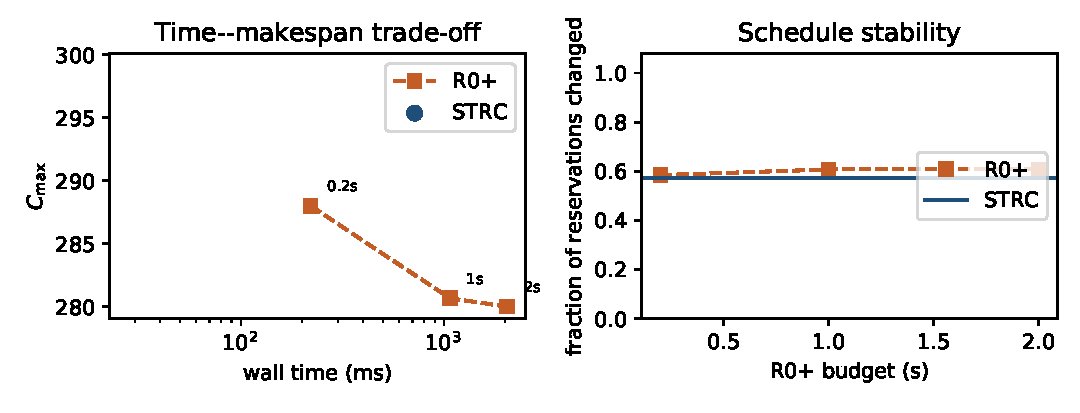
\includegraphics[width=\linewidth]{figures/fig_strc_e5}
\caption{E5: the budget sweep of R0+ without rewriting finished occupancies, against
the fixed point of bounded repair (\texttt{congested\_8x4x4}, means over \(3\)
random seeds).
Left: algorithm runtime against \(C_{\max}\); the two curves do not intersect.
Right: the rewrite fraction of occupancies, with both methods around six tenths.}
\Description{Two panels side by side. In the left panel the horizontal axis is the
algorithm runtime on a logarithmic scale and the vertical axis the makespan:
warm-started global rescheduling without rewriting finished occupancies decreases
slightly with the budget, bounded repair is a single point at the upper left, the
two do not intersect, and global rescheduling is slightly lower at every budget
point. The right panel shows the rewrite fraction of occupancies, with both methods
around six tenths rather than one hundred per cent against six tenths.}
\label{fig:e5}
\end{figure}

The makespan of bounded repair is worse over the whole range, while its algorithm
runtime is two to three orders of magnitude lower (taking the
\(\MsRepairMed\)\,ms of level-1 rerouting against a budget of
\(0.2\)--\(2\)\,s; see Figure~\ref{fig:e5}, left).
This runtime difference comes from a single rerouting pass without restarting the
search and is \emph{not} to the credit of the boundary drawn on the impact set---
Section~\ref{sec:cheap} establishes this with the equally fast RA comparison.
The rewrite fraction, meanwhile, is already at the same \ResFracRtwo\ order as
R0+'s (for fewer rewrites see the RA comparison of Section~\ref{sec:cheap}: the two
fractions here are already close, so stability cannot be read off this table).
When the response must be at the order of milliseconds, bounded repair can restore
feasibility; when a stoppage of seconds is permitted, warm-started global
rescheduling without rewriting finished occupancies is still ahead on makespan,
though by a far smaller margin than the variant that reschedules from \(t=0\).
\(C_{\max}\) is the primary measure in this field and is therefore what we report.
The comparison mentioned in Section~\ref{sec:vs_r0} means that the two are each
usable under a constraint on \emph{algorithm runtime}, not that there is a budget
range in which the \(C_{\max}\) of R2 is better.

The R0+ of this table uses the fixed-prefix decoding of Section~\ref{sec:vs_r0} and
does not rewrite occupancies that have already finished.
In the audit of ``finished occupancies may not be rewritten'', the violations are
\(\RzeroPastLo\) at each of the \(9\) budget points of the small example and of the
congested example; where a downstream operation of the same job had already
dispatched a vehicle while an upstream one still needed retiming, forcing the
original vehicle and replanning only the tail after \(t_{\mathrm{now}}\) preserves
the historical empty prefix.
Bounded repair remains uniformly zero on the same cells.
Compared with the older ``reschedule from \(t=0\)'' comparison, the gap in
\(C_{\max}\) has narrowed markedly and the rewrite fraction is no longer one
hundred per cent against six tenths; but the order of the two is unchanged and
there is still no crossover. What used to be mixed into the gap---``rewriting
occupancies that have already finished''---has been removed, and what remains is
the margin of global reassignment and resequencing over a single rerouting pass.
As far as the contributions are concerned, this section establishes one
\emph{qualification} only: the net effect of the reservation impact set does not lie
in makespan, and its place of application is the millisecond band; what the net
effect actually is is answered by the RA comparison of Section~\ref{sec:cheap}.

\subsection{E7: comparisons within the millisecond band}
\label{sec:cheap}

The comparison of the previous section is a warm-started population search with a
budget of \(0.2\)--\(2\)\,s. Using it alone leaves one question open:
\emph{how much of that ``two to three orders of magnitude'' reading comes from the
reservation impact set, and how much merely from the comparison taking longer?}
This section fills in the two intermediate rungs of the ladder, the faster global
recomputations.

\begin{itemize}[leftmargin=1.5em,itemsep=0.25em]
\item \textbf{RS (global right shift).} Paths, assignments and sequence are all
unchanged, and the unfinished occupancies are pushed back as a whole by a delay
\(\Delta\), chosen just large enough for every movable occupancy on the obstructed
corridor to land after the blockage window.
Occupancies already finished are not rewritten
(\(t_{\mathrm{end}}\le t_{\mathrm{now}}\) is immovable), as in R2; because the shift
is uniform, every gap either stays the same or grows, and since all constraints are
of ``\(\ge\)'' type, a feasible solution is obtained without any rerouting.
It is one extreme of ``\emph{drawing no boundary on the impact set}'': even
rerouting is given up (Section~\ref{sec:rw_aor}).
\item \textbf{RD (re-decoding of the original chromosome).} The machine assignment
and the sequence are kept, and the same fixed-prefix decoding as R0+ is run on a
routing layer loaded with the blockage. It is \emph{the faster global recomputation}
in this implementation; it does not change the chromosome, so it is faster than R0+
and has less freedom to reassign and resequence.
\item \textbf{RA (no restriction of the scope by the impact set, but rerouting
retained).} Every occupancy \emph{unfinished} after \(t_{\mathrm{now}}\) is brought
into the rewritable set, and then \emph{exactly the same} rerouting replay as R2 is
run. It is the other extreme of ``drawing no boundary on the impact set'': unlike
RS it retains rerouting, and therefore differs from R2 only in which occupancies may
be rewritten. The two share one rerouting procedure, neither touches occupancies
already finished, and both use the same blockage.
It is therefore the \emph{only} comparison in this paper that isolates the
reservation impact set on its own---the difference between the two methods contains
no contribution from the rerouting procedure, the protocol or the implementation.
RA is already the maximal rewritable set and needs no escalation after a failure.
\end{itemize}

E3 compares two \emph{different} objects for the boundary to be drawn on (the
operation-precedence graph vs the reservation impact set), whereas RA asks:
\emph{should the scope be restricted by the impact set at all?}

\begin{table}[t]
\centering
\caption{E7, comparisons within the millisecond band (\(\NPairs\) pairs, protocol as
in E3: single-window blockage on a busy corridor,
\(t_{\mathrm{now}}=0.35\,C_{\max}^{0}\), no escalation for R2). All four methods are
feasible on \(\NPairs/\NPairs\).
``Finished violated'' counts the cells on which a finished occupancy was rewritten;
``rewritable'' is the share, among the occupancies unfinished after
\(t_{\mathrm{now}}\), that the method brings into the rewritable set; the last column
is that method's \(C_{\max}\) record against R2. RA and R2 differ only in which
occupancies may be rewritten, so the difference between those two rows is entirely
attributable to the reservation impact set.
This table \emph{must not} be read alongside Table~\ref{tab:e5}, which covers two
instances only.}
\label{tab:cheap}
\small
\begin{tabular}{@{}lcccccc@{}}
\toprule
Method & \makecell{Finished\\violated} & \makecell{ms\\(median)} & \makecell{Mean\\degradation} & \makecell{Rewrite\\fraction} & Rewritable & \makecell{vs R2\\win/tie/loss} \\
\midrule
RS global right shift & \ShiftBad     & \MsShift    & \(58.8\%\) & \ResFracShift    & ---   & \(7/16/27\) \\
RD re-decoding        & \RedecodeBad  & \MsRedecode & \(49.0\%\) & \ResFracRedecode & ---   & \(22/14/14\) \\
RA no impact boundary & \ShiftBad     & \MsAllFuture & \(49.9\%\) & \ResFracAllFuture & \(1.00\) & \(0/46/4\) \\
R2 bounded repair     & \ShiftBad     & \MsCheapRtwo & \(49.8\%\) & \ResFracCheapRtwo & \ClosureShareMean & --- \\
\bottomrule
\end{tabular}
\end{table}

Table~\ref{tab:cheap} gives four readings.

\textbf{First, among the methods that return a feasible plan, the only one faster
than bounded repair is the global right shift, and it is worse both in makespan and
in rewrite fraction.} (R1, with the boundary drawn on the operation-precedence
graph, is faster still, but it restores feasibility on \FeasRone\ and is no
candidate.)
RS needs only \MsShift\,ms, about half of R2; the price is a mean makespan
degradation of \(58.8\%\) (against \(49.8\%\) for R2), a per-cell record of
\WinVsShift\ (R2 win/tie/loss), and more rewritten occupancies rather than
fewer (\ResFracShift\ against \ResFracCheapRtwo)---a uniform shift changes the
times of every unfinished occupancy.
To make the right shift \emph{selective}---delaying only the vehicles genuinely
affected and leaving the rest alone---one would first have to know which occupancies
are affected, which is exactly the scope this paper delineates.
\textbf{The right shift can dispense with a boundary on the impact set precisely
because it has given up choosing.}

\textbf{Second, the faster global recomputation still takes longer than one bounded
repair.} The median runtime of RD is \MsRedecode\,ms, \RedecodeRatio\ times that of
R2. This reading is independent of the search configuration: in any decoding-based
search, evaluating a candidate costs at least one decoding.
The ``two to three orders of magnitude'' of the previous section is therefore
\emph{not} an artefact of choosing a slower comparison---replacing the comparison by
the faster rung of the same implementation, bounded repair is still faster.

\textbf{Third, once finished occupancies are no longer rewritten, the makespans of
RD and R2 are indistinguishable on this sample, but RD rewrites more.}
Over the whole table, R2's record against it is \WinVsRedecode\ (win/tie/loss), with
mean degradations of \(49.8\%\) against \(49.0\%\). The difference does not survive
testing: the mean paired difference is \(+0.006\) with a bootstrap \(95\%\) interval
\([-0.007,\,0.019]\) straddling \(0\); the two-sided Wilcoxon signed-rank test gives
\(p=0.12\) (\(36\) cells with a non-zero difference); and the mean \(C_{\max}\) ratio
is \(0.997\) with an interval \([0.988,\,1.007]\), which straddles \(1\) as well.
We therefore report only ``no difference observed'' and give no direction.
Violations on finished occupancies already stand at \RedecodeBad: for a downgraded
downstream operation the original vehicle is now forced and only the tail after the
decision time is replanned, so the historical empty prefix is no longer lost.
Even where RD is slightly ahead on the per-cell count, therefore, this must not be
written up as ``coming from rewriting occupancies that have already finished''---it
is the margin of global rerouting over a single rerouting pass, with the same
chromosome and only the future scheduled.
RD's rewrite fraction is \ResFracRedecode, higher than R2's
\ResFracCheapRtwo: fewer rewrites remain on the side that draws the boundary on the
impact set.

\textbf{Fourth, fewer rewrites can be read only from R2 against RA, and what is read
is stability alone.} RA and R2 differ only in which occupancies may be rewritten, so
this pair of readings answers directly what drawing the boundary on the impact set
buys in net terms.
On average the reservation impact set leaves out only \(1-\ClosureShareMean\) of the
unfinished occupancies relative to the trivial upper bound (per cell
\ClosureShareLo--\(1.00\); on the \(6\) cells attaining \(1.00\) the impact set
\emph{is} the set of all unfinished occupancies and the two methods coincide).
It is precisely this difference of less than a tenth that brings the rewrite fraction
down from \ResFracAllFuture\ to \ResFracCheapRtwo: a mean reduction of
\RAStabMean\ and a median reduction of \RAStabMed, per cell \RAStabWTL\ (R2 more
stable/tie/less stable), two-sided Wilcoxon signed-rank \(p=\RAStabP\).
The effective sample size must be stated: the \(6\) coincident cells are not
comparisons between the two methods; removing them leaves \(44\) cells, a per-cell
record of \RAStabWTLNet\ and a mean reduction of \RAStabMeanNet\ (the number of cells
with a non-zero difference for Wilcoxon is \(32\) under either accounting); removal
makes the estimated reduction \emph{larger}, so reporting over \NPairs\ cells is the
more conservative side. The direction is highly consistent and the \emph{magnitude
is small}---on the single counterexample cell R2 in fact rewrites \(0.007\) more,
which is recorded as well.
Meanwhile the algorithm runtimes are almost identical (\MsCheapRtwo\ against
\MsAllFuture\,ms) and so are the makespans (mean ratio \RACmaxRatio, per-cell R2
win/tie/loss \WinVsAllFuture, never worse, the most favourable cell being
\RACmaxLo).

These three items together are the point. \textbf{The identical runtimes show that
the millisecond-level response comes from a single rerouting pass without restarting
the search, and not from the reservation impact set (readings in
Table~\ref{tab:cheap} of this section; a single rerouting pass is itself existing
practice, see Table~\ref{tab:position}).
The identical makespans show that the impact set is not an optimization device.
The markedly lower rewrite fraction shows that drawing the boundary delivers exactly
the quantity promised by Proposition~\ref{prop:outside}: the corridor, interval and
vehicle of the occupancies outside the set are unchanged.}
The role of the impact set is to \emph{mark which occupancies need not be changed}.
The magnitude grows as the impact set excludes more, the direction is consistent, but
the excluded set alone accounts for only part of it---even counting every occupancy
forbidden to be rewritten, that does not make up the whole
\(\ResFracAllFuture-\ResFracCheapRtwo\) gap, and the remainder comes from differences
in the rerouting outcome itself once the modifiable set shrinks; we do not decompose it
further:
on an instance where the impact set is close to all unfinished occupancies
(\texttt{congested\_8x4x4}, rewritable share \(0.94\)) the reduction is only
\(0.010\), whereas on an instance where more is excluded
(\texttt{S8x4x4\_mid}, \(0.91\)) it reaches \(0.118\).
% selfcheck:allow-num 0.91 is the rewritable share of that instance; it is numerically equal to \ScaleCloAliveHi (the upper end of the E8 per-level means) but comes from a different source.
Two instances cannot fix a proportionality, and all that can be said is the
direction; the per-cell distribution follows.

Let us write this direction up as a post hoc rule.
Figure~\ref{fig:worth} plots the \(\NPairs\) pairs with the rewritable share
\(\mathrm{Cl}/|R^{\circ}|\) on the horizontal axis and the reduction in rewrite
fraction of R2 relative to RA on the vertical axis.
Taking \(\mathrm{Cl}/|R^{\circ}|\ge\WorthThresh\) on this sample: above that line,
\WorthHighN\ cells have a mean reduction of \WorthHighMean, and below it,
\WorthLowN\ cells have a mean reduction of \WorthLowMean.
The reductions have all fallen to zero once the share rises above \(\WorthVanish\),
but for two different reasons: on the \(6\) cells whose share is exactly \(1.00\) the
impact set is the set of all unfinished occupancies and the two methods
\emph{coincide}; on the remaining cells the share is below \(1.00\) and the reduction
is nevertheless \(0\), which is measured rather than identical by construction.
This is a post hoc stratification whose threshold is chosen on this table, and no
extrapolated theorem is claimed; it answers ``when is drawing the boundary on the
impact set still worthwhile'', not the structural prediction of the impact-set size
(which remains unestablished, Section~\ref{sec:e4}).

\begin{figure}[t]
\centering
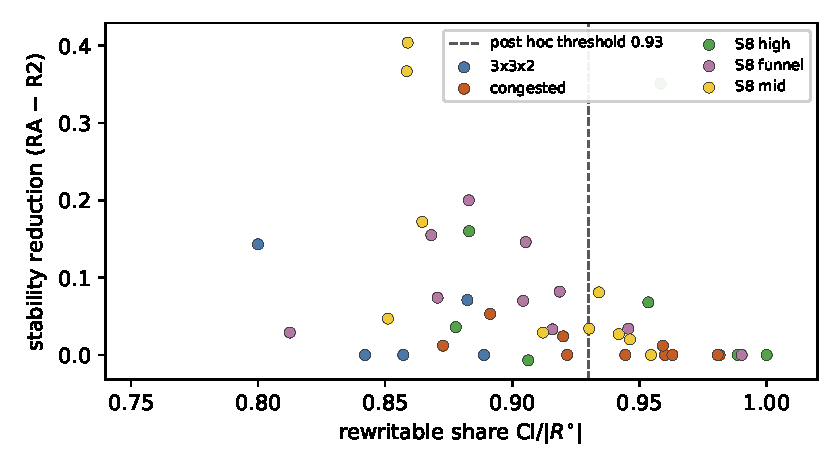
\includegraphics[width=0.92\linewidth]{figures/fig_strc_worth}
\caption{E7 post hoc rule: rewritable share against stability reduction
(\(\NPairs\) pairs, R2 against RA).
The dashed line is the in-sample threshold \(\WorthThresh\); a positive value on the
vertical axis means a lower rewrite fraction once the boundary is drawn on the
impact set.}
\Description{A scatter plot whose horizontal axis is the share of the reservation
impact set in the unfinished occupancies and whose vertical axis is the extra
fraction of occupancies rewritten when no boundary is drawn on the impact set,
relative to when it is; the five instances are distinguished by colour and a vertical
dashed line marks \WorthThresh. The points run broadly from upper left to lower
right.}
\label{fig:worth}
\end{figure}

Reading the four methods together closes the matter as follows: under the two
constraints ``do not rewrite occupancies that have already finished'' and ``respond
at the order of milliseconds'', \textbf{the net benefit of drawing the boundary on
the impact set shows up in the amount of rewriting alone---at equal speed and equal
makespan, not drawing it means rewriting about \(6\) percentage points more
occupancies (about a twelfth more in relative terms)}, and it includes \emph{no}
advantage in speed or in makespan.
This layer answers the net benefit of drawing the boundary; ``whether the object the
boundary is drawn on stands up'' is supported by
Sections~\ref{sec:e1}--\ref{sec:e3}.
Once the runtime constraint is relaxed, the shorter makespan still comes from the
warm-started search (Section~\ref{sec:e5}), but that is no longer the millisecond
band.

\subsection{A sweep over the disturbance scale}
\label{sec:scale}

Table~\ref{tab:scale} and Figure~\ref{fig:scale} report the \(\varphi\) sweep
(\texttt{congested\_8x4x4}, \(\NSeeds\) random seeds; R0+ budget \(2\)\,s).
The per-level readings are in the table; \(C_{\max}\) is still better for R0+
throughout, in agreement with Section~\ref{sec:e5}.
On the small example \texttt{example\_3x3x2} every cell is likewise feasible
(\(\NSeeds\) random seeds \(\times\) five values of \(\varphi\)), with bounded
repair at the order of \(1\)\,ms and a runtime ratio of
\(\SpeedLo\times\)--\(\SpeedHi\times\) (per-cell extremes across the two
instances).
Here the denominator is the measured wall clock of bounded repair while the
numerator is the \emph{budget} of R0+, and R0+ is better on \(C_{\max}\), so this is
not a ``speed-up'' and constitutes no comparison at equal quality
(Section~\ref{sec:protocol} has already declared that the methods are not compared
at a common budget level).

Bounded repair here has scope escalation switched on, so this section is not
directly comparable with E3/E5: escalation is the step that pulls the feasibility
rate to \(100\%\) and has precedents of its own (Section~\ref{sec:rw_aor}).
This section \emph{supports none of the contributions} and establishes one
qualification only: even when the disturbance fraction rises to \(\varphi=1\) (every
future operation disturbed), the algorithm runtime stays at the order of tens of
milliseconds and does not collapse with size; and this runtime comes from the single
rerouting pass and is \emph{not} to the credit of the boundary drawn on the impact
set (Section~\ref{sec:cheap}).

\begin{table}[t]
\centering
\caption{Comparison across the disturbance scale (\texttt{congested\_8x4x4},
averaged over \(\NSeeds\) random seeds).
Bounded repair includes escalation; the R0+ budget is \(2\)\,s. Dispersion is
reported as an interquartile range: the spread of the STRC runtime over the whole
sweep is \ScaleMsMin--\ScaleMsMax\,ms, and the per-level IQR of the R0+ \(C_{\max}\)
lies between \ScaleCmaxIqrLo\ and \ScaleCmaxIqrHi.
\textbf{At the two smallest levels the within-level IQR of the ``runtime ratio''
column already exceeds the between-level movement of that column, so it is to be read
as an order of magnitude only and does not indicate a trend in \(\varphi\).}
That column is the per-level mean of the \emph{per-cell} ratios (pair first, then
aggregate), and therefore does not equal the ratio of the two neighbouring column
means---the two necessarily differ by the convexity of \(1/x\), so please use the
per-cell data when recomputing.
The numerator is the wall-clock \emph{budget} of R0+ rather than its measured
runtime, so this is not a comparison at equal quality
(Section~\ref{sec:protocol}).}
\label{tab:scale}
\small
\begin{tabular}{@{}rcccc@{}}
\toprule
\(\varphi\) & STRC feasible & STRC\,ms & R0+ \(C_{\max}\) & Runtime ratio \\
\midrule
\(0.10\) & \(100\%\) & \(9.1\)  & \(103.5\) & \(406\times\) \\
\(0.25\) & \(100\%\) & \(11.1\) & \(107.0\) & \(325\times\) \\
\(0.50\) & \(100\%\) & \(8.6\)  & \(111.8\) & \(333\times\) \\
\(0.75\) & \(100\%\) & \(8.4\)  & \(125.8\) & \(254\times\) \\
\(1.00\) & \(100\%\) & \(10.7\) & \(148.1\) & \(203\times\) \\
\bottomrule
\end{tabular}
\end{table}

\begin{figure}[t]
\centering
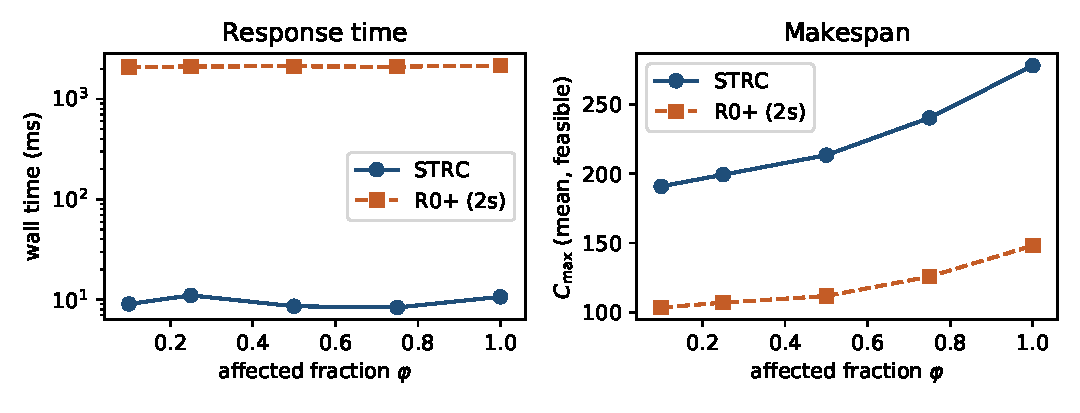
\includegraphics[width=\linewidth]{figures/fig_strc_scale}
\caption{Sweep over the disturbance scale (\texttt{congested\_8x4x4},
\(\NSeeds\) random seeds): the algorithm runtime (logarithmic axis) and the makespan
of bounded repair and of R0+ as functions of \(\varphi\). The curves are per-level
means, and the dispersion convention is that of Table~\ref{tab:scale} (interquartile
range); on the runtime side the spread over the whole sweep is
\ScaleMsMin--\ScaleMsMax\,ms, always at the order of tens of milliseconds, and this
is the only reading on which this section rests its argument.}
\Description{Two curves as functions of the disturbance fraction. The algorithm
runtime is drawn on a logarithmic vertical axis: bounded repair stays at the order of
tens of milliseconds and does not collapse as the fraction rises, while global
rescheduling sits on the fixed two-second budget line. On the makespan side, global
rescheduling rises slowly with the disturbance fraction but stays below bounded repair
throughout.}
\label{fig:scale}
\end{figure}

\subsection{E8: extrapolation in instance size}
\label{sec:instscale}

The previous section swept the scale of the \emph{disturbance}, with the instance
fixed at \(8\) jobs and \(4\) machines. This section changes dimension: the
disturbance protocol is fixed and the instance itself is scaled up.
The crux of this question is not runtime---that it does not collapse is to be
expected---but \textbf{whether the impact-set share rises towards \(1\) with size, so
that ``bounded'' becomes an empty word}.

The size sequence takes \(2k\) jobs, \(k\) machines and \(k\) vehicles for
\(k=4,\dots,10\), that is from \(8\times4\times4\) to
\(\ScaleJobsHi\times\ScaleMachHi\times\ScaleMachHi\), giving \(\ScaleKs\) levels
\(\times\) \(\NSeeds\) random seeds \(=\ScalePairs\) pairs.
The congestion level, the heterogeneity, the flexibility, the
transport-to-processing time ratio, the load/unload minimum cut and the remote cut
are all calibrated to the same targets, and \emph{only the size varies}. The three
comparisons are defined as in Section~\ref{sec:cheap}.

\begin{table}[t]
\centering
\caption{E8, sweep over instance size (\(\ScaleKs\) levels \(\times\) \(\NSeeds\)
random seeds).
``Impact set'' is the share of the reservation impact set in the \emph{whole table};
the attainable upper bound of that ratio is \(|R^{\circ}|/|R|\), whose mean in this
batch is about \ScaleAliveShare; with the rewritable set as denominator it is
\ScaleCloAliveLo--\ScaleCloAliveHi\ (see the body).
Runtimes are medians, and the ``RD/R2'' column is the ratio of those two
\emph{medians}; the monotonicity discussed in the body uses per-level means of the
per-cell pairs, and the two conventions move alike between levels but differ in
value.
The last column is R2's \(C_{\max}\) record against RS.}
\label{tab:instscale}
\small
\begin{tabular}{@{}lrccccc@{}}
\toprule
Size & \(|R|\) & Impact set & R2\,ms & RD\,ms & RD/R2 & R2 vs RS \\
\midrule
\(8\times4\times4\)    & \(148\) & \(0.561\) & \(2.9\)  & \(4.4\)  & \(1.5\times\) & \(7/1/2\) \\
\(10\times5\times5\)   & \(172\) & \(0.485\) & \(3.2\)  & \(6.1\)  & \(1.9\times\) & \(9/0/1\) \\
\(12\times6\times6\)   & \(230\) & \(0.481\) & \(4.5\)  & \(10.7\) & \(2.4\times\) & \(7/1/2\) \\
\(14\times7\times7\)   & \(281\) & \(0.492\) & \(6.1\)  & \(14.5\) & \(2.4\times\) & \(8/0/2\) \\
\(16\times8\times8\)   & \(291\) & \(0.534\) & \(6.4\)  & \(16.4\) & \(2.6\times\) & \(10/0/0\) \\
\(18\times9\times9\)   & \(356\) & \(0.535\) & \(8.2\)  & \(26.4\) & \(3.2\times\) & \(10/0/0\) \\
\(20\times10\times10\) & \(402\) & \(0.476\) & \(10.4\) & \(34.2\) & \(3.3\times\) & \(10/0/0\) \\
\bottomrule
\end{tabular}
\end{table}

The per-level readings are in Table~\ref{tab:instscale}.

\textbf{The impact-set share does not deteriorate with size, but the worry about
``approaching \(1\)'' is only answered once the denominator is changed.}
The seven levels of \(\mathrm{Cl}/|R|\) fluctuate between \ScaleCloLo\ and
\ScaleCloHi\ and are not monotone (the first level is the highest and the last the
lowest, while the fifth and sixth come back above \(0.53\)).
The denominator must be made explicit here, or too strong a conclusion will be read
off: \(\mathrm{Cl}\) takes only the occupancies unfinished after
\(t_{\mathrm{now}}\), whereas the mean \(|R^{\circ}|/|R|\) in this batch is only
\ScaleAliveShare, so the attainable upper bound of \(\mathrm{Cl}/|R|\) is not \(1\)
but about \ScaleAliveShare---using it to answer the question above is beside the
point.
With the rewritable set as denominator, the seven levels of
\(\mathrm{Cl}/|R^{\circ}|\) fall in \ScaleCloAliveLo--\ScaleCloAliveHi\ (per cell up
to \(1.00\)), of the same order as the \ClosureAliveFrac\ of the main batch in
Sections~\ref{sec:e6} and~\ref{sec:cheap}.
What this section supports is therefore that \emph{the share does not deteriorate
with size}, and \emph{not} that ``bounded'' is generous in absolute terms---the
latter has already been denied in Remark~\ref{rem:minimality}.
Nor is this an asymptotic claim: seven levels are insufficient to fit any growth
rate, and all that can be said is that over this range it has not degraded.

\textbf{The algorithm runtime grows faster than the total number of occupancies.}
As \(|R|\) grows by a factor of \(2.7\), R2's median runtime grows from \(2.9\) to
\ScaleMsHi\,ms, a factor of \(3.6\), and remains at the order of tens of
milliseconds; seven levels fix no exponent, so only the ratio of the two endpoints is
reported, and it is written neither as ``linear'' nor as ``superlinear''.
The number of cells feasible with level-1 rerouting is \ScaleFeasFirst; the single
failing cell (\(10\times5\times5\), seed \(42\)) is caught by scope escalation in
round \(3\), with a total runtime of \(12.0\)\,ms and the same makespan as the
level-1 attempt, so the final feasibility is \ScaleFeasAll.

\textbf{The gap between the two comparisons widens with size.} The runtime ratio of
the faster global recomputation to bounded repair rises from \ScaleRatioLo\(\times\)
to \ScaleRatioHi\(\times\)---the larger the instance, the less a full recomputation
pays.
Only the two endpoints are reported here: the per-level ratio is \emph{not monotone}
(the per-level mean of the per-cell pairs dips at \(k=6\to 7\)).
The two endpoints differ by \(1.8\), whereas the interquartile range within any level
does not exceed \(0.74\) and the sampling fluctuation of a per-level mean over
\NSeeds\ cells is far smaller than that span, so \emph{the overall rise} is not
noise; the shape of the growth, however, we do not report.
Against the right shift, which draws no boundary on the impact set, R2's
\(C_{\max}\) record is \(10/0/0\) at each of the last three levels, while at the
first four levels it varies between \(7\) and \(9\) wins with no monotone pattern;
each level has only \NSeeds\ cells, so only the clean sweeps of the last three levels
are reported and no trend is claimed.

\textbf{Limits of the convention.} This size sequence has one congestion level and one
instance seed (the instance at each level is itself generated with seed \(42\)), so
what it tests is the \emph{size} dimension and it cannot replace the comparison over
congestion structures in the main batch of Section~\ref{sec:protocol}; nor were the
sweeps of Sections~\ref{sec:e6} and~\ref{sec:scale} re-run on this batch.
As far as the contributions are concerned, this section adds one qualification in the
\emph{size direction} to the boundedness of C2: the share is not diluted over these
seven levels, but this bears on no net benefit and constitutes no asymptotic
conclusion.

\subsection{Reproduction on the external-layout batch}
\label{sec:pubrepro}

Once the second batch of Section~\ref{sec:protocol} replaces the provenance of the
layouts by an external source, the E1/E2/E3/E5 readings on the \(\NPubPairs\)
instance--seed pairs agree \emph{item by item in direction} with those of the main
batch: the operation-precedence graph returns an empty scope on \PubPassMiss,
structural containment (that is, zero leakage) holds on \PubPassClosed, and the fields
outside the set are unchanged entry by entry on \PubPassInvar; under the boundary
ablation the number of cells feasible with level-1 rerouting is \PubFeasRone, while
with the boundary drawn on the reservation impact set it is \PubFeasRtwo.
Under the E1 protocol, the per-layout median impact-set share falls in
\PubEoneFracLo--\PubEoneFracHi; the comparable reading in the main batch is the
median \EoneFracMed\ over the \NPairs\ pooled pairs (\EoneCloLo--\EoneCloHi\ is the
spread of the per-instance \emph{means}, a different convention that should not be
read directly against the preceding clause).
The external batch is slightly lower overall, but both are of the order of about a
half, and the shortfall is of the same order as the between-instance variation (see
the caption of the figure in Section~\ref{sec:e1}); we offer no attribution for it.
The trade-off against global rescheduling is unchanged as well: R0+ has the better
\(C_{\max}\) at \PubEfiveNoCross\ of the budget points, with the remaining \(1\)
point a tie (\texttt{LyuL6\_8m}, seed \(2024\), budget \(0.2\)\,s) and none worse.
This batch runs the same E5 code with the same parameters as the main batch, which is
why Section~\ref{sec:e5} reads the two batches together over \(\EfiveCells\)
instance--seed cells; the tied cell also satisfies the monotonicity argument of that
section, and the crossover still does not exist.

The value of this batch lies not in new performance numbers but in answering
``whether these phenomena hold only on layouts we designed ourselves'': the three
readings above hold equally on a batch of topologies not chosen by us, so the object
layer of C1 and C2 does not depend on our layout design.
The only conclusion this batch revises is structural predictability
(Section~\ref{sec:e4}), and that was a negative result to begin with.

\subsection{Summary}
\label{sec:exp_summary}

The readings of this chapter are grouped by the contribution layer they support; the
limitations of each, and which layer each does and does not threaten, are collected
in Section~\ref{sec:limitations}.

\textbf{The object layer} (C1, C2: on what the boundary is drawn, and whether the set
so drawn is uniquely determined) is supported by four groups of readings.
Under corridor blockage the scope on the operation-precedence graph is empty while the
original schedule is indeed infeasible (E1, \(\PassMiss\) on \(\NPairs\) pairs);
the reservation impact set is closed under the dependency edges and the fields outside
it are unchanged entry by entry (E2, \(\PassClosed\) and \(\PassInvar\));
replacing only the object the boundary is drawn on under one and the same rerouting
procedure moves the rate at which feasibility is restored from \(\FeasRone\) to
\(\FeasRtwo\) (E3), so that feasibility comes from the object the boundary is drawn on
and not from the quality of the rerouting procedure; and in the cross of four
disturbance types with two ways of drawing the boundary the A/B dichotomy holds without
exception, while on Class A the reservation impact set uniformly contains the
operation-precedence boundary (E6).
Propositions~\ref{prop:miss}--\ref{prop:outside} give the corresponding structural
statements, of which Proposition~\ref{prop:outside} remains a sufficient condition
only.

\textbf{The net-benefit layer} (C3: what drawing the boundary this way buys) is
supported by one group of readings only: switching to the comparison that does not
restrict the scope by the impact set (RA, with the same rerouting as R2 and likewise
never touching occupancies already finished), algorithm runtime and \(C_{\max}\) barely
change, while the rewrite fraction rises from \ResFracCheapRtwo\ to
\ResFracAllFuture\ (per cell \RAStabWTL, \(p=\RAStabP\);
Section~\ref{sec:cheap}).
Hence the millisecond-level response comes from the single rerouting pass and not from
the impact set, and \textbf{fewer rewrites can be read only from this comparison}.
Against warm-started global rescheduling, bounded repair is better on \(C_{\max}\) on
no cell, and relaxing the budget produces no crossover (E5); E7 then removes the doubt
that ``the comparison simply took longer''.

The remaining two groups of readings support no contribution and only add
qualifications: the scale sweep has reached \(\ScaleJobsHi\) jobs and
\(\ScaleMachHi\) machines, and the impact-set share with the rewritable set as
denominator has not deteriorated with size (E8); structural predictability is a
negative result (E4).
The second batch of instances (\(\NPubPairs\) pairs) only tests whether the phenomena
above depend on the layouts we chose ourselves, and E1, E2, E3 and E5 all reproduce
item by item.

%% =====================================================================
\section{Conclusion}
\label{sec:conclusion}
%% =====================================================================

This paper makes three contributions. \textbf{First}, it identifies a class of damage
beyond the reach of the operation-precedence graph: a corridor blockage changes no
operation assignment, and the scope delineated by affected operations is empty while
the original schedule is indeed infeasible (\(\PassMiss\) on \(\NPairs\) pairs,
Section~\ref{sec:e1}).
\textbf{Second}, it defines the rescheduling scope as the reservation impact set
(\STRC): once the dependency relations are given, whether an occupancy belongs to the
set is uniquely determined, and no dependency edge leads from inside the set to outside
it (\(\PassClosed\), \(\PassInvar\), Section~\ref{sec:e2}); this layer does not depend
on the net-benefit readings below.
\textbf{Third}, it gives a local recovery matched to this boundary and keeps straight
where each reading comes from: replacing only the object the boundary is drawn on under
one and the same rerouting procedure moves the rate at which feasibility is restored
from \(\FeasRone\) to \(\FeasRtwo\) (Section~\ref{sec:e3}), so that feasibility comes
from the object the boundary is drawn on and not from the quality of the rerouting
procedure.

The several mechanisms that make up the impact set---yielding relations, rerouting
inside the set while keeping the plan outside it, and enlarging the rewritable scope
after a failure---have each appeared in the existing literature
(Section~\ref{sec:rw_claim}), and we do not claim them as contributions. What this
paper claims is this: the operation-precedence graph contains, by definition, no
yielding relations among corridor occupancies, and therefore cannot reach a
disturbance that merely invalidates occupancies; once the scope is moved onto the
reservation dependency graph, the occupancies that must be rewritten are uniquely
determined by the given order, rather than by a heuristic radius.

When the rewritable set is changed from the reservation impact set to ``every
occupancy unfinished after \(t_{\mathrm{now}}\)'' and everything else is left
untouched, algorithm runtime and makespan barely move, while the rewrite fraction rises
from \ResFracCheapRtwo\ to \ResFracAllFuture\ (Section~\ref{sec:cheap}).
Hence the millisecond-level response comes from a single rerouting pass without
restarting the search; \textbf{fewer rewrites can be read only from this comparison,
and what it delivers is the quantity promised by Proposition~\ref{prop:outside}: the
occupancies outside the set keep the original plan}.
The magnitude of the benefit depends on how far the impact set falls short of that
trivial upper bound, and so tends to vanish as the two approach each other.

\subsection{Limitations}
\label{sec:limitations}

The four items below are ordered by their bearing on the readings above, and
Section~\ref{sec:future} gives a direction for each.

\begin{enumerate}[leftmargin=1.6em,itemsep=0.35em]
\item \textbf{The makespan is worse than that of warm-started global rescheduling
without rewriting finished occupancies, and relaxing the budget produces no
crossover.}
Bounded repair trades makespan for algorithm runtime, and this disadvantage does not
reverse as the budget is relaxed on the \(\EfiveCells\) instance--seed cells measured
(Section~\ref{sec:e5}).
This item \textbf{threatens} the layer of ``the net benefit of drawing the boundary on
the reservation impact set'' and \textbf{does not threaten} the layer of ``which
occupancies must be rewritten is uniquely determined by the structure'': fewer rewrites
can be read only from the comparison with RA and not from the comparison with R0+
(Section~\ref{sec:cheap}).

\item \textbf{For the reservation impact set, the guarantee of
Proposition~\ref{prop:outside} is only a sufficient condition, the dependency edge set
has not been tested exhaustively and independently, the rewritable set is not tight, and
its size cannot be predicted by static measures that depend on the network alone.}
The impact set covers about \(\ClosureAliveFrac\) of the occupancies unfinished after
\(t_{\mathrm{now}}\), and we make no minimality claim
(Remark~\ref{rem:minimality}); the magnitude of the net benefit depends on how far the
impact set falls short of that trivial upper bound, so the benefit tends to vanish as
the two approach each other.
The family of static cuts has already been ruled out in Section~\ref{sec:e4}, but that
negative result bears only on ``the static cuts can explain the size of the impact
set'' and does not amount to ``network geometry is unrelated to the size of the impact
set''.
This item \textbf{threatens} the strength and the tightness of the guarantees at the
object layer and \textbf{does not threaten} the diagnostic reading that ``drawing the
boundary on the operation-precedence graph returns an empty scope''.

\item \textbf{The implementation covers less than the problem range described in the
body: Class-B disturbances are answered by rerouting alone, Class A additionally opens
vehicle swap and reassignment but not a change of operation order, and by Assumption A3
only one response is made.}
Opening up the operation order degenerates towards global rescheduling, and ``bounded''
thereby loses its boundary; disturbance streams, prediction error and rolling response
are all untouched.
The size dimension has been swept to \(\ScaleJobsHi\) jobs and \(\ScaleMachHi\)
machines with no rise in the impact-set share, but the number of levels swept cannot
support any asymptotic statement.
This item \textbf{threatens} extrapolation of the readings to larger sizes and to
continuous disturbances and \textbf{does not threaten} the readings already reported
within the protocol.

\item \textbf{An absent external reference: this class of study has no public benchmark
that could be substituted in, the provenance of the instances is externalized only to
the level of topology, and the readings have not been reproduced on a second
implementation.}
The public instance families~\cite{homayouni2021production,bilge1995time} publish
transport times as a matrix of machine-to-machine travel times rather than as a
network, and of the \(11\) layouts the two families provide between them, checked
one by one, not one could be recovered as an undirected corridor graph
consistent with the published matrix, so \(R\), \(G_R\), \(\mathrm{Cl}(\cdot)\) and
Class-B disturbances cannot be defined on them at all
(Section~\ref{sec:protocol}).
The second batch of instances is constructed from the appendix layouts of Lyu et
al.~\cite{lyu2019approach}, so the layouts are no longer of our design, but the per-leg
travel times and the job data still come from us, so they cannot be used to reproduce
the reference values of Lyu et al.\ or of van Os and Basten~\cite{vanos2026exact},
and their coverage is narrower than that of the main batch.
This item \textbf{threatens} external validity and \textbf{does not threaten} the
relative readings among the comparisons within one implementation.
\end{enumerate}

\subsection{Future work}
\label{sec:future}

The four items below correspond one to one with the four limitations of the previous
section.

\textbf{One: facing the makespan disadvantage over the whole range} (limitation
\(1\)).
The rewriting of finished occupancies by the prefix decoding has already been
eliminated in the main batch (\(\RzeroPastLo\) violations at the \(18\) budget points of
E5, and \RedecodeBad\ for RD in E7).
What remains of limitation 1 is \(C_{\max}\) itself, and we do not evade it by
switching to a differently weighted measure.
Narrowing the gap would require limited reassignment or resequencing while still not
rewriting finished occupancies, and that degenerates towards global rescheduling.

\textbf{Two: making the guarantee for the reservation impact set more complete and
tighter, and establishing a characterization of its size} (limitation \(2\)).
\emph{Completeness}: abutment has been folded into the yield edges, and after re-running,
the probe leaks \ProbeLeaks.
The next step is to probe with a different form of disturbance (shortening an occupancy,
say, or delaying by more than \(1\) unit) rather than to add the same edge again.
\emph{Tightness}, pointing at a smallest rewritable set: define minimality under a fixed
repair capability and give the gap between the impact set and it---an unavoidable step in
carrying ``bounded'' from a sufficient condition to a tight bound; since the impact set
currently covers about \(\ClosureAliveFrac\) of the unfinished occupancies, that gap may
be considerable.
\emph{Characterizing the size} currently rests on a single post hoc rule (the rewritable
share, Figure~\ref{fig:worth}), which varies with the schedule; it must be replaced by a
family of measures computable before the disturbance.
Section~\ref{sec:e4} has already ruled out the family of static cuts---it takes constant
values on real layouts, whereas changing only the machine configuration on one and the
same network makes it move: on the \(4\times 4\) network, going from \(4\) to \(5\)
machines moves it by \PubCloSpread, and on the \(5\times 5\) network three
configurations (\(6\), \(7\) and \(8\) machines) move it by \PubCloSpreadBig.
The latter suggests the direction: what appears to matter is the \emph{spatial
distribution of demand}, not the throughput the network provides.
The next candidate is the temporal density of corridor occupancies in the neighbourhood
of \(t_{\mathrm{now}}\), for instance the number of overlapping occupancies of the
disturbed corridor within its busy window, and the out-degree of that corridor in the
yield graph. Such quantities vary with the schedule and are no longer purely
topological, so the phrase ``predictability'' must be changed accordingly to predicting
the size given the layout \emph{and the current schedule}.

\textbf{Three: relaxing Assumption A3} (limitation \(3\); A3 is the single, fully
observed disturbance).
The next step is not to open up resequencing further but to relax that assumption, and
to examine whether the impact set accumulates and swells under successive disturbances,
and whether an explicit ``re-homing'' step is needed between two repairs.

\textbf{Four: externalizing the time calibration as well} (limitation \(4\)).
The provenance of the layouts has settled half of this; completing the other half still
requires an instance family that publishes \emph{both an exclusive network and per-leg
durations}, and a sweep over self-assigned edge weights is no substitute.
As for a second independent implementation, it needs no separate project: it can be done
along with any of the reproductions above.

%% Housekeeping: funding, acknowledgements and conflict of interest, as is customary
%% for journals.
%% The acks environment of acmart is hidden automatically in review/anonymous mode, so
%% an anonymous submission needs no manual deletion.
\begin{acks}
This work was supported by <to be supplied: funding programme name and grant number>.
The authors thank the anonymous reviewers for their comments on the experimental
conventions and on the boundaries of the conclusions.
\end{acks}

\section*{Conflict of interest statement}
The authors declare that they have no conflict of interest related to the work
reported here.

\bibliographystyle{ACM-Reference-Format}
\bibliography{reference-base}

\end{document}
